\section{Phenomenology}\label{sec:Phenom}

The theoretical differential decay rate for an initial $\Bs$ (Eq.~\ref{eq:decayrate}) is described by a sum of ten terms, corresponding to the four polarization (0, $\parallel$, $\perp$, S) amplitudes of the $\Kp\Km$ system and their interference~\cite{Liu:2013nea}. Each of these can be factorized into a time dependent and an angular dependent components
\begin{equation}\label{eq:decayrate}
 \frac{d^{4}\Gamma(\Bs\to\jpsi\phi)}{dtd\ctk d\ctl d\phi}\propto\sum^{10}_{k=1}h_{k}(t)f_{k}(\Omega).
\end{equation}
The time dependent functions $h_{k}(t)$ are given as:
\begin{equation}\label{eq:decayrate_time}
 h_{k}(t)=N_{k}e^{-\Gamma t}\left[a_{k}\cosh\frac{\DGs t}{2}+b_{k}\sinh\frac{\DGs t}{2}+c_{k}\cos(\dms t)+d_{k}\sin(\dms t)\right].
\end{equation}
The $\dms$ is the mass difference between the $\Bs$ mass eigenstates, $\dms=M_{H}-M_{L}$. The coefficients $N_{k}$ and $a_{k}$,..., $d_{k}$ can be expressed in terms of $\phis$ and four complex transversity amplitudes $A_{f}$ at $t = 0$. The label $f$ takes the values $\{\perp, \parallel, 0\}$ for the three P-wave amplitudes and S for the one S-wave amplitude. In the fit we parameterize each $A_{f}(0)$ by its magnitude squared $|A_{f}(0)|^{2}$ and its phase $\delta_{f}$, and adopt the convention $\delta_{0} = 0$, $|A_{\perp}|^{2} + |A_{0}|^{2} + |A_{\parallel}|^{2} = 1$ and $f_{S} = |A_{S}|^{2}/(|A_{S}|^{2} + |A_{\perp}|^{2} + |A_{0}|^{2} + |A_{\parallel}|^{2} ) = |A_{S}|^{2}/(|A_{S}|^{2} + 1)$. For a particle produced in a $\Bs$ flavour eigenstate, $\Bs$ and $\Bsb$, the coefficients in Eq.~\ref{eq:decayrate_time} and the angular functions $f_{k}(\Omega)$ are given in Table~\ref{tab:AngTimeFunction}  where 
\[
 S = −\frac{2|\lambda|}{1+|\lambda|^{2}}\sin(\phis),\quad D = −\frac{2|\lambda|}{1+|\lambda|^{2}}\cos(\phis)\quad\text{and}\quad C = \frac{1-|\lambda|^{2}}{1+|\lambda|^{2}}.
\]
 We allow for possible $\CP$ violation in mixing and in the decay amplitudes through the inclusion of the parameter $\lambda$, which is defined as $\lambda=\eta_{f}\frac{q}{p}\frac{\bar{A}_{f}}{A_{f}}$, where $q$ and $p$ are the complex coefficients connecting the mass and flavour eigenstates, $|B_{L,H}\rangle = p|\Bs\rangle\pm q|\Bs\rangle$, $\bar{A}_{f}$ is the analog of $A_{f}$ for $\Bsb$ and $\eta_{f}$ is the $\CP$-eigenvalue of the final state. With these conventions, $\phis = -\arg(\lambda)$.
 
 By performing an angular analysis of the decay products one can separate statistically the contributions from the different amplitudes. Such an analysis requires a measurement of the three decay product angles $\Omega=\{\theta, \varphi, \psi\}$ defined in Fig.~\ref{fig:Phen:Angles}. In the coordinate system of the $\jpsi$ rest frame (where the $\phi$ and $\Bs$ meson move in the $x$ direction, the $z$ axis is perpendicular to the decay plane of $\phi\to\Kp\Km$, with $p_{y}(\Kp)\geq0$), the transversity polar and azimuthal angles ($\theta$, $\varphi$) describe the direction of the $\ep$. In the rest frame of the $\phi$ meson, the angle $\psi$ is the angle between $x$ axis and the $\Kp$ momentum. 

\begin{sidewaystable}[h]
   \caption{
The angular and time dependent functions used in Equations~\ref{eq:decayrate} and \ref{eq:decayrate_time}.
}
%     \small{
\begin{center}\begin{tabular}{c|c|c|c|c|c|c}
    \hline
    $k$    & $f_{k}(\theta_{e},\theta_{K},\phi_{h})$ & $N_{k}$ & $a_{k}$ & $b_{k}$ &  $c_{k}$ & $d_{k}$ \\ 
    \hline
    1   & $2\cos^{2}\theta_{K}\sin^{2}\theta_{e}$ & $|A_{0}(0)|^{2}$ &  1 & $D$ & $C$ & $-S$\\
    2   & $\sin^{2}\theta_{K}(1-\sin^{2}\theta_{e}\cos^{2}\phi_{h})$ & $|A_{\parallel}(0)|^{2}$ &  1 & $D$ & $C$ & $-S$\\
    3   & $\sin^{2}\theta_{K}(1-\sin^{2}\theta_{e}\sin^{2}\phi_{h})$ & $|A_{\perp}(0)|^{2}$ &  1 & $-D$ & $C$ & $S$\\
    4   & $\sin^{2}\theta_{K}\sin^{2}\theta_{e}\sin2\phi_{h}$ & $|A_{\parallel}(0)A_{\perp}(0)|^{2}$ &  $C\sin(\delta_{\perp}-\delta_{\parallel})$ & $S\cos(\delta_{\perp}-\delta_{\parallel})$ & $\sin(\delta_{\perp}-\delta_{\parallel})$ & $\cos(\delta_{\perp}-\delta_{\parallel})$\\
    5   & $\frac{1}{2}\sqrt{2}\sin2\theta_{K}\sin2\theta_{e}\cos\phi_{h}$ & $|A_{0}(0)A_{\parallel}(0)|^{2}$ & $\cos(\delta_{\parallel}-\delta_{0})$  & $D\cos(\delta_{\parallel}-\delta_{0})$ & $C\cos(\delta_{\parallel}-\delta_{0})$ & $-S\cos(\delta_{\parallel}-\delta_{0})$\\
    6   & $-\frac{1}{2}\sqrt{2}\sin2\theta_{K}\sin2\theta_{e}\sin\phi_{h}$ & $|A_{0}(0)A_{\perp}(0)|^{2}$ & $C\sin(\delta_{\perp}-\delta_{0})$  & $S\cos(\delta_{\perp}-\delta_{0})$ & $\sin(\delta_{\perp}-\delta_{0})$ & $D\cos(\delta_{\perp}-\delta_{0})$\\
    7   & $\frac{2}{3}\sin^{2}\theta_{e}$ & $|A_{S}(0)|^{2}$ &  1 & $-D$ & $C$ & $S$\\
    8   & $\frac{1}{3}\sqrt{6}\sin\theta_{K}\sin2\theta_{e}\cos\phi_{h}$ & $|A_{S}(0)A_{\parallel}(0)|^{2}$ & $C\cos(\delta_{\parallel}-\delta_{S})$  & $S\sin(\delta_{\parallel}-\delta_{S})$ & $\cos(\delta_{\parallel}-\delta_{S})$ & $D\sin(\delta_{\parallel}-\delta_{S})$\\
    9   & $-\frac{1}{3}\sqrt{6}\sin\theta_{K}\sin2\theta_{e}\sin\phi_{h}$ & $|A_{S}(0)A_{\perp}(0)|^{2}$ & $\sin(\delta_{\perp}-\delta_{S})$  & $-D\sin(\delta_{\perp}-\delta_{S})$ & $C\sin(\delta_{\perp}-\delta_{S})$ & $S\sin(\delta_{\perp}-\delta_{S})$\\
    10   & $\frac{4}{3}\sqrt{3}\cos\theta_{K}\sin^{2}\theta_{e}$ & $|A_{S}(0)A_{0}(0)|^{2}$ & $C\cos(\delta_{0}-\delta_{S})$  & $S\sin(\delta_{0}-\delta_{S})$ & $\cos(\delta_{0}-\delta_{S})$ & $D\sin(\delta_{0}-\delta_{S})$\\
    \hline
  \end{tabular}\end{center}
%   }
\label{tab:AngTimeFunction}
\end{sidewaystable}

   \begin{figure}[hbt]
  \begin{center}
    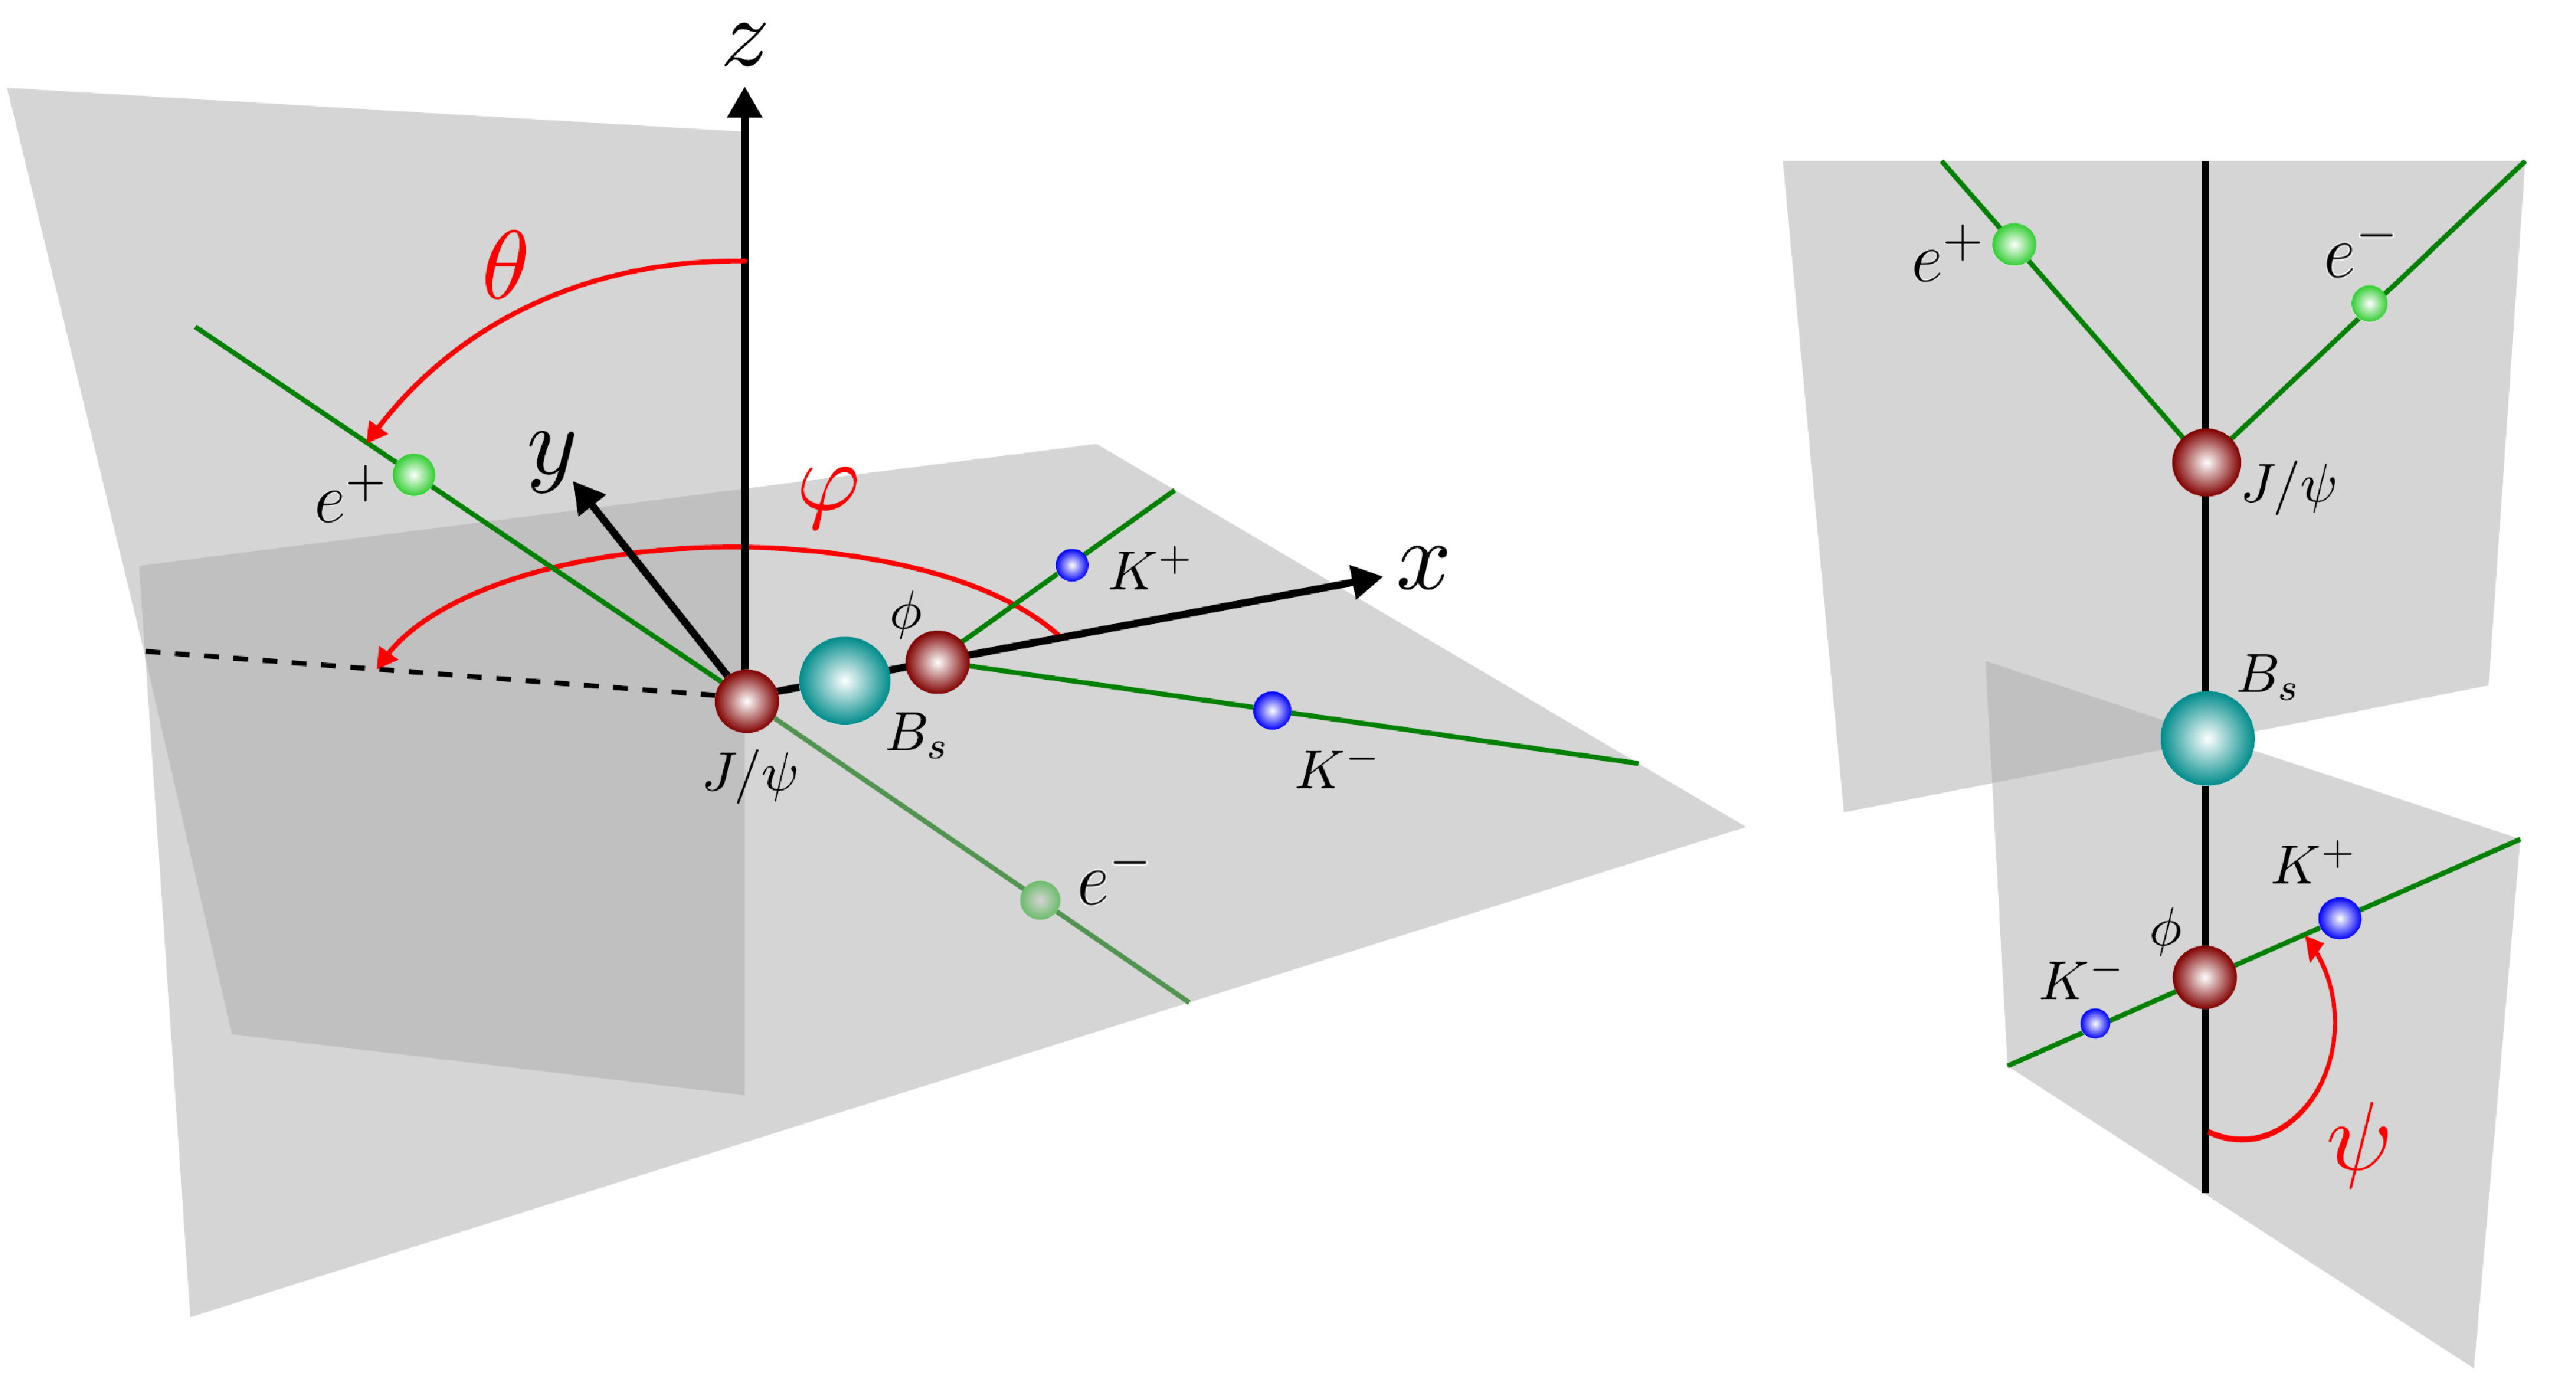
\includegraphics[width=0.8\linewidth]{Phenomenology/Angles_ee.pdf}
  \end{center}
  \caption{
   The angle definitions: $\theta$ is the angle formed by the positive lepton ($\ep$) and the $z$ axis, in the $\jpsi$ rest frame. The angle $\varphi$ is the azimuthal angle of $\ep$ in the same frame. In the $\phi$ meson rest frame, $\psi$ is the angle between $\vec{p}(\Kp)$ and $-\vec{p}(\jpsi)$. The definitions are the same for both $\Bs$ or a $\Bsb$ decays.   
}
  \label{fig:Phen:Angles}
\end{figure}
\clearpage


\section{Data samples, event reconstruction, selection and trigger}\label{sec:Data}
\subsection{Data samples}

The candidates of $\Bs\to\jpsi(\epem)\phi$ used in this analysis are selected from the data sample taken in 2011 at $\sqs$ = 7~$\tev$ and 2012 at $\sqs$ = 8~$\tev$. They are reconstructed with version 14 of the reconstruction software (Reco14). The 2011 data are stripped with version 21r1 (Stripping21r1-Merging-DV-v36r1), while the 2012 are stripped with 21 (Stripping21-Merging-DV-v36r1). In both cases, we use the Radiative stream and the {\tt StrippingBs2JpsieePhiDetachedLine}. 
The tuples are made on the GRID using $\davinci$ v37r2p4 with the track momentum scale calibration applied. Further processing is performed offline\footnote{Details of the code can be found in Appendix~\ref{sec:app:AnaCode}.} including application of the selection cuts, selection of single candidate for events with multiple ones, as well as calculation of the sWeights, the procedure for which is described in Sec.~\ref{sec:BsFit}. The integrated luminosity is 0.9875~$\invfb$ in 2011 and 2.0399~$\invfb$ in 2012.

\subsection{MC samples}\label{subsec:MC}

 The Monte Carlo (MC) samples are produced with Sim08 and listed in Table~\ref{tab:MC}. For each event type, half of the sample is produced with $\pythia$6, half with $\pythia$8, each of them being split equally into "magnet up" and "magnet down". The decays are preformed with $\evtgen$ and $\photos$++. The stripping is in "flagging mode", the reconstruction is "Reco14a", no prescale and no spillover are applied. For 2011-like MC samples, the trigger is simulated with $\moore$~v12r8g3 and TCK~0x40760037. For 2012 MC samples, the trigger is simulated with $\moore$~v14r8p1 and TCK~0x409f0045. The main physics parameters used in the simulation are summarized in Table~\ref{tab:MCparam}. A track level smearing has been applied to the simulated events to match the momentum resolution of the data.
   \begin{table}[hbt]
  \caption{
    Monte Carlo samples used in the analysis. All samples are produced with Sim08. The number of events quoted is the sum of $\pythia$6(MagUp)+$\pythia$6(MagDown)+$\pythia$8(MagUp)+$\pythia$8(MagDown), for 2011 plus 2012.}
    \small{
\begin{center}\begin{tabular}{lccc}
    \hline
    Decay Channel                         &  & Event type & Tot. number of events       \\ 
    \hline
    Bs$\_$Jpsiphi,ee=CPV,update2012,DecProdCut   &  & 13154001 &  20M\\
    incl$\_$Jpsi,ee=DecProdCut &  & 24152001  & 20M \\
    Bu$\_$JpsiX,ee=JpsiInAcc & &  12952000 & 13.4M \\
    Bd$\_$JpsiX,ee=JpsiInAcc & &  11453001 & 11.6M \\
    Bs$\_$JpsiX,ee=JpsiInAcc & &  13454001 & 11M \\
    Lb$\_$JpsiX,ee=JpsiInAcc & &  15454101 & 11.4M \\
    Lb$\_$JpsipK,ee=phsp,DecProdCut & &  15154001 & 10M \\
    Lb$\_$Jpsippi,ee=phsp,DecProdCut & &  15154021 & 10M \\
    \hline
  \end{tabular}\end{center}
  }
\label{tab:MC}
\end{table}

 \begin{table}[hbt]
  \caption{
    Decay model parameters for the Sim08 MC signal sample used in this analysis. The parameter values are based on those reported in Ref.~\cite{Aaij:2013oba}.}
    \small{
\begin{center}\begin{tabular}{cc}
    \hline
    Parameter                         &  Value       \\ 
    \hline
    $\dms$   &  17.8~$\invps$\\
    $\DGs$  & 0.0917~$\invps$ \\
    $\Gs$   & 0.6653~$\invps$ \\
    $\phis$ & 0.07~$\rad$ \\
    $|A_{0}(0)|^{2}$ & 0.722 \\
    $|A_{\parallel}(0)|^{2}$ & 0.480 \\
    $|A_{\perp}(0)|^{2}$ & 0.499 \\
    $\delta_{\parallel}-\delta_{0}$ & 3.30~$\rad$\\
    $\delta_{\perp}-\delta_{0}$ & 3.07~$\rad$\\
    \hline
  \end{tabular}\end{center}
  }
\label{tab:MCparam}
\end{table}
 
 \subsection{Event Selection}\label{subsec:EvtSel}
 
 For the events selected by the stripping line, first the $\jpsi\to\epem$ decay is reconstructed, then the $\phi\to\Kp\Km$ decay and finally the $\Bs\to\jpsi\phi$ is looked for.
 Table~\ref{tab:Selection} summarizes the requirements in the stripping line as well as additional preselection requirements that are applied.

  \begin{table}[hbt]
  \caption{
    Selection criteria for $\BsToJPsiPhi$ candidates in Stripping21{r1} and preselection. 
}
    \small{
\begin{center} \begin{tabular}{|c|c|c|c|}
    \hline
 Decay mode & Cut parameter & Stripping & Preselection  \\
  \hline
 $\jpsi\to\epem$ & $\Delta ln\mathcal{L}_{e\pi}$ & $>$0 & - \\
 & $\chisq_{\text{track}}$/ndf($e$) & $<$5 & $<$4 \\
 & $\chisqip(e)$ & - & $>$0 \\
 & $\pt(e)$ & $>$500~$\mevc$ & - \\
 & $\chisqvtxndf(\jpsi$) & $<$15 & - \\
 & $\pt(\jpsi)$ & - & $>$400~$\mevc$ \\
 & $m(\jpsi)$ & $\in$[2500, 3300]~$\mevcc$ & - \\
 \hline
  $\phi\to\Kp\Km$ & $\Delta ln\mathcal{L}_{K\pi}$ & - & $>$0 \\
  & $\chisq_{\text{track}}$/ndf($K$) & - & $<$4 \\
  & $\pt(K)$ & - & $>$200~$\mevc$ \\
  & $p(K)$ & - & $>$3000~$\mevc$ \\
  & GhostProb$_{\text{track}}(K)$ & - & $<$0.5 \\
 & $\pt(\phi)$ & $>$1000~$\mevc$ & - \\
 & $\chisqvtxndf(\phi$) & $<$15 & $<$9 \\
 & $m(\Kp\Km)$ & $\in$[990, 1050]~$\mevcc$ & - \\
 \hline
  $\Bs\to\jpsi\phi$ & $m(\Bs)$ & $\in$[4500, 6000]~$\mevcc$ & $\in$[4600, 6000]~$\mevcc$ \\
 & $\chisqvtxndf(\Bs$) & $<$10 & - \\
 & $\chisqip(\Bs$) & - & $<$20 \\
 & $t$ & $>$0.3~$\ps$ & - \\
 \hline
    \end{tabular}\end{center}
  }
\label{tab:Selection}
\end{table}

\subsection{Trigger}\label{subsec:Trigger}

The stripping and final event selection are chosen in a way to not affect the decay time acceptance. The trigger is the only source of the time dependent inefficiency is the trigger. For this reason the trigger lines are divided into two categories: a decay time unbiased and biased trigger lines. The trigger categories are defined as follows:
 \begin{enumerate}
  \item Unbiased: {\tt L0ElectronDecision$\_$TOS} or {\tt L0HadronDecision$\_$TOS}
  \item Biased: ({\tt Hlt1TrackAllL0Decision$\_$TOS} and ({\tt Hlt2Topo(2,3,4)BodyBBDTDecision$\_$TOS} or {\tt Hlt2TopoE(2,3,4)BodyBBDTDecision$\_$TOS})) or {\tt Hlt2IncPhiDecision$\_$TOS} 
 \end{enumerate}

 The unbiased triggers correspond to approximately 72$\%$ and 81$\%$ of the selected events in data and MC, respectively, as shown in Fig.~\ref{fig:TimeTrigger}.
 \begin{figure}[hbt]
  \begin{center}
    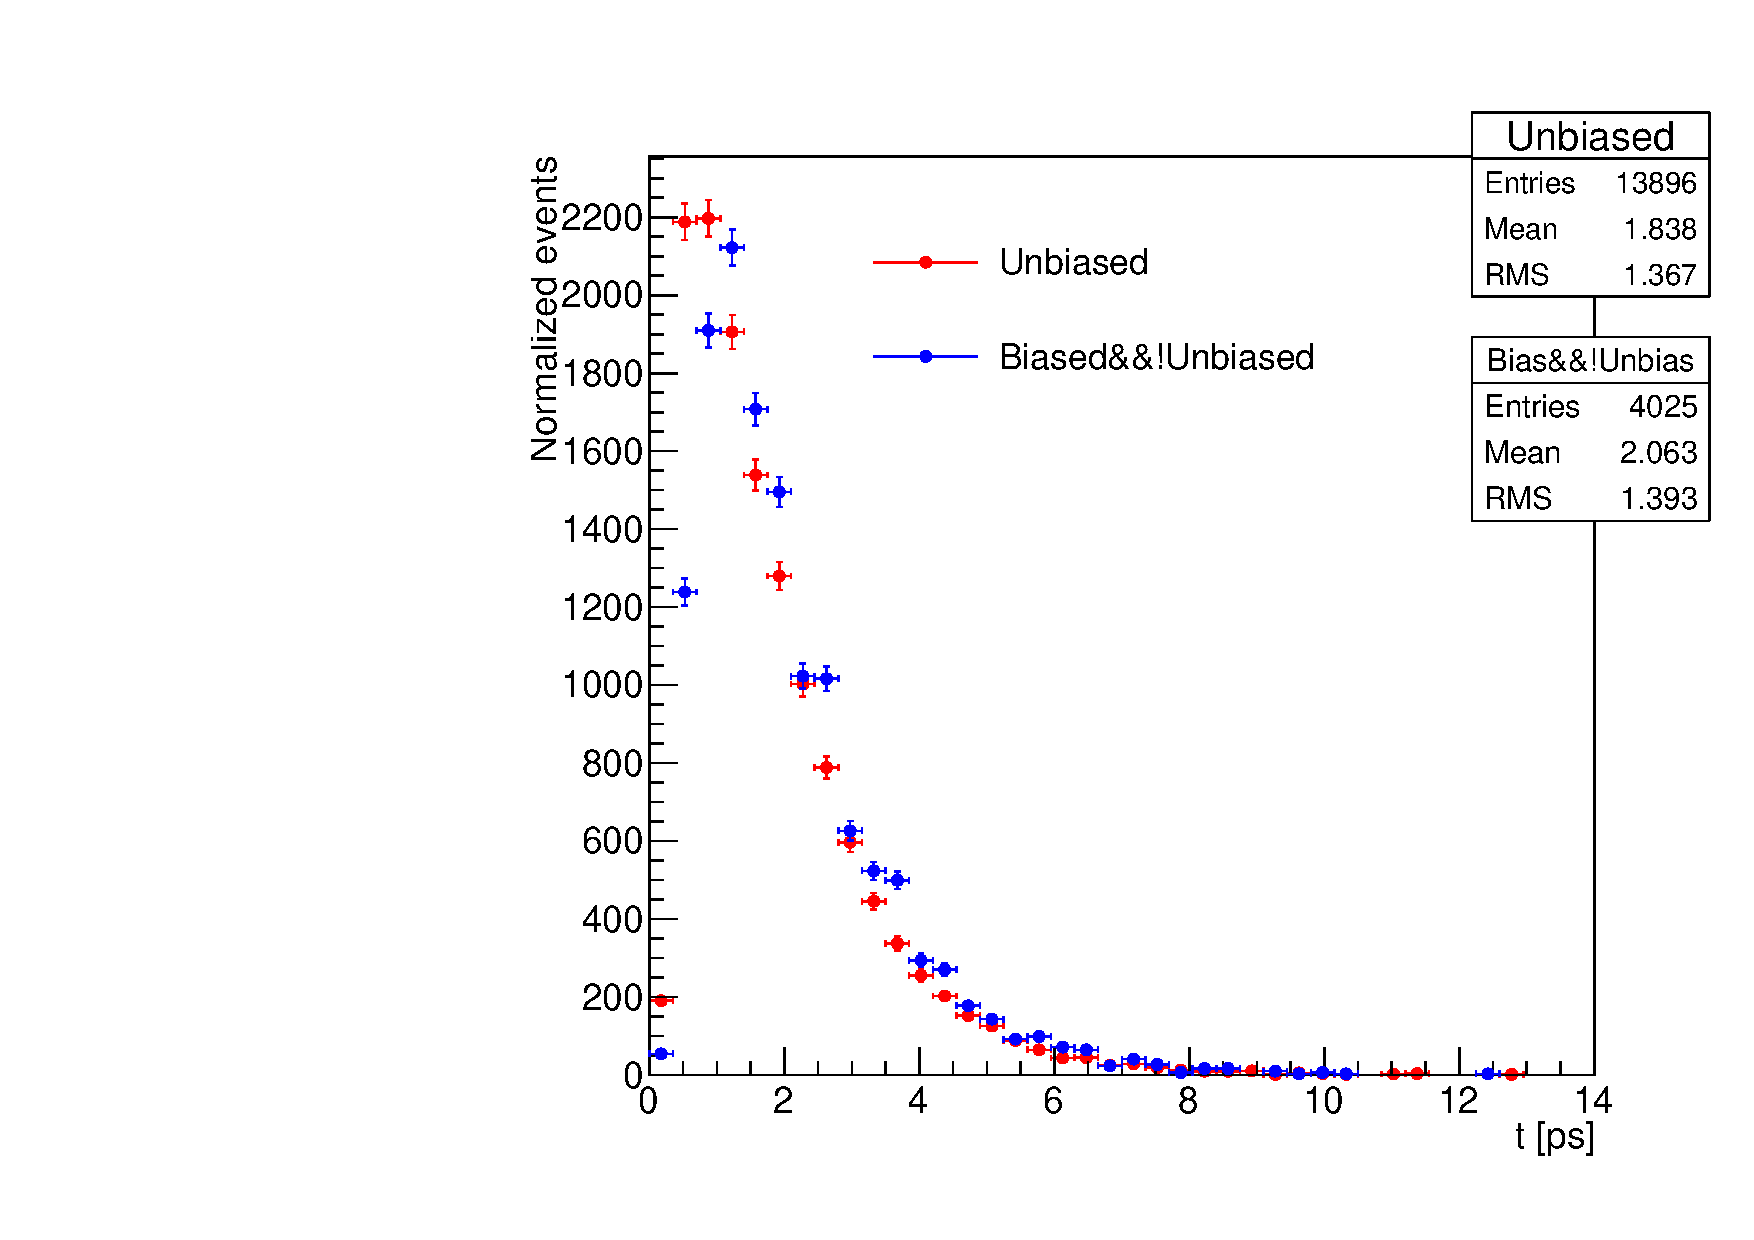
\includegraphics[width=0.48\linewidth]{Trigger/RDfull.pdf}\put(-115,-4){(a)}
    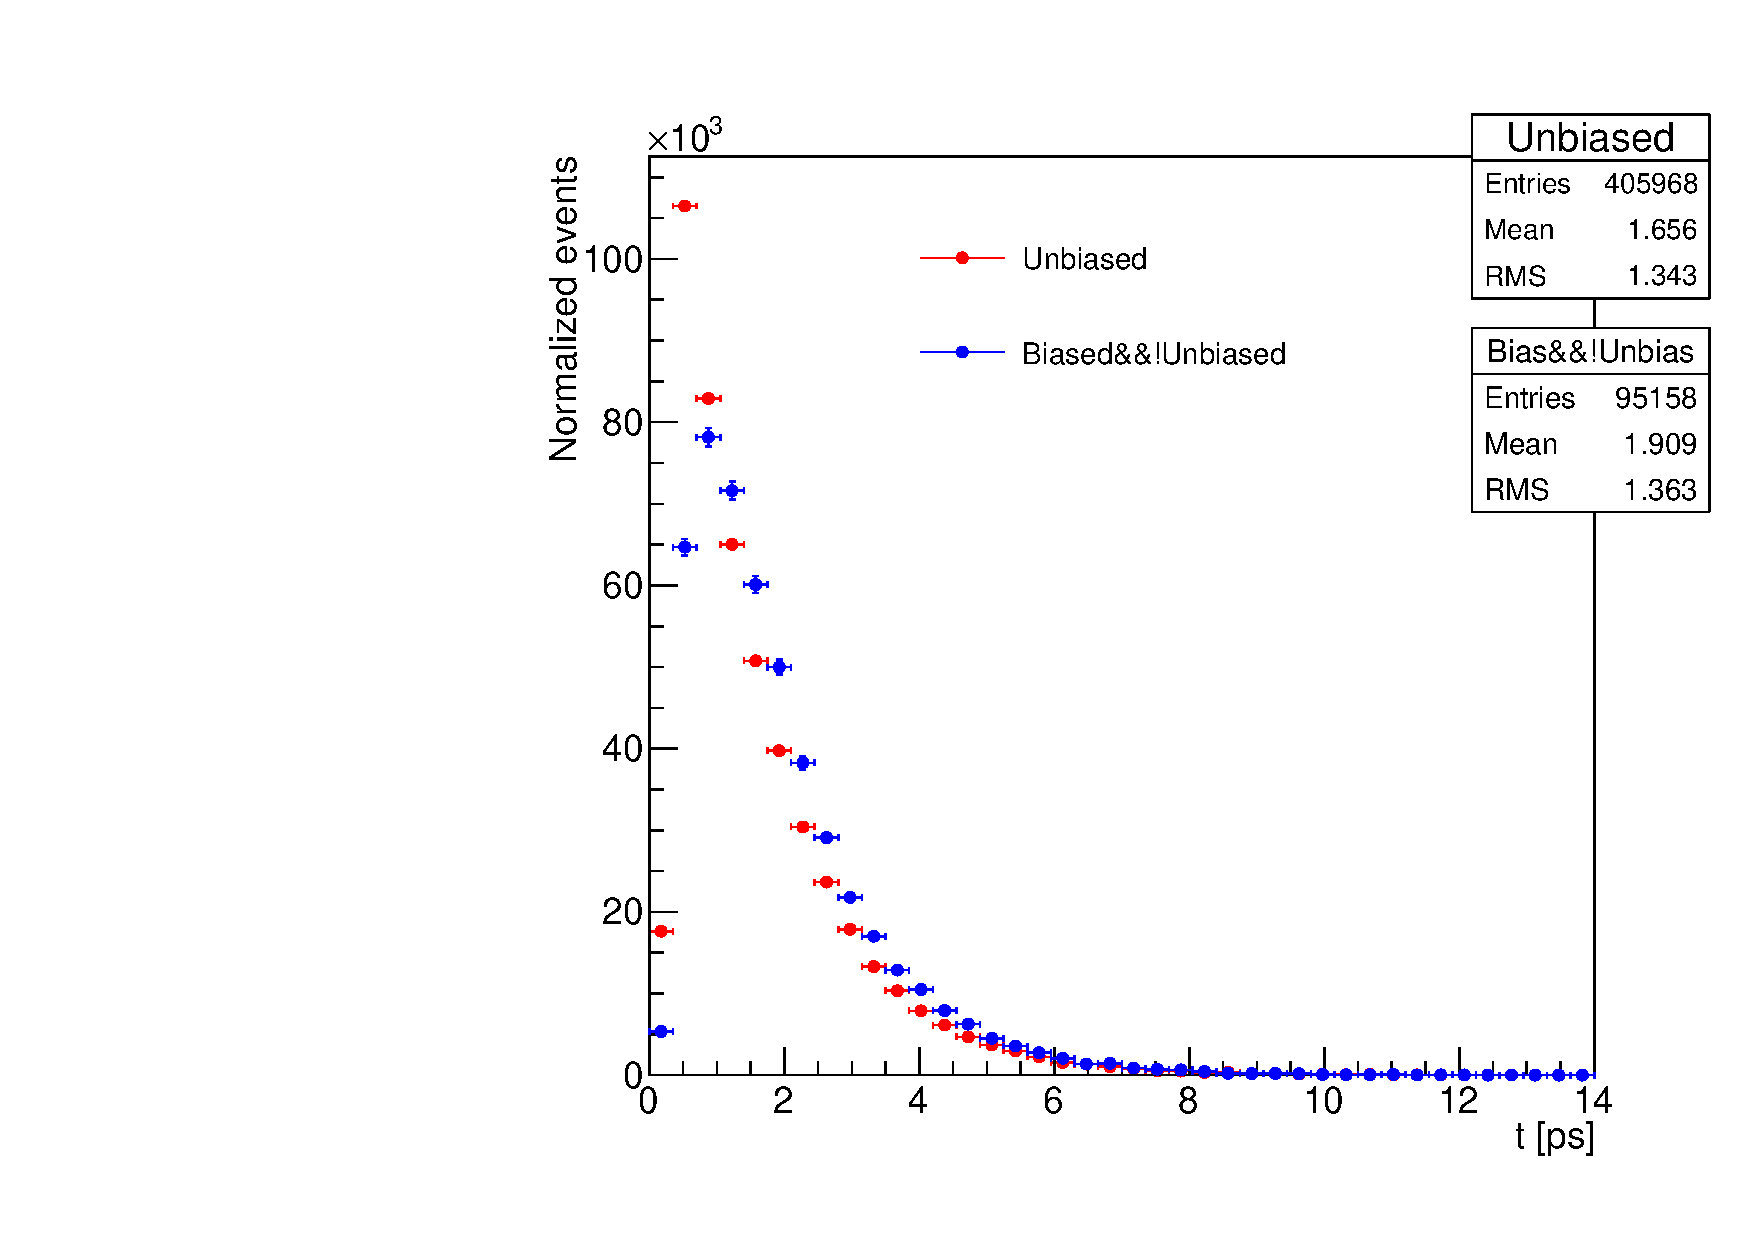
\includegraphics[width=0.48\linewidth]{Trigger/MCfull.pdf}\put(-115,-4){(b)}
  \end{center}
  \caption{
   The decay time distribution of the events which are triggered by the unbiased triggers (red) and by the biased ones but not by unbiased (blue) for data (a) and MC (b).  
}
  \label{fig:TimeTrigger}
\end{figure}
 
 The procedure to derive the decay time dependent efficiencies of these trigger categories are described in Sec.~\ref{sec:TimeAcc}. 
 
 \subsection{Monte Carlo reweighting}\label{subsec:MCreweight}
 While there is in general a good agreement between data and MC for the samples used in this analysis, a significant difference exists in the event occupancy being largely under-estimated in the simulated data. The occupancy correlates to the invariant mass shape of the signal as the correction of the electron momenta for the bremsstrahlung photons emitted before the magnet depends on proper measurement of particles energies in the electromagnetic calorimeter (ECAL). Therefore, it is important to property include this effect in the MC. A way to accommodate data and MC difference is to use the scintillating pad detector (SPD) hits multiplicity distribution, which is highly correlated to the event occupancy. Therefore, a reweighting of the simulated events is applied in order to match their SPD multiplicity distribution to the LHCb data. The procedure used for this analysis is the same as described in Ref.~\cite{Borsato:2014-009}.
 
The discrepancy in the SPD hit multiplicity between data and MC is presented in Fig.~\ref{fig:nSPDHits}(a). The reweighting is performed separately for 2011 and 2012 as the average number of interactions per bunch crossing was different in the two years. The weights, which are applied to the simulation, are shown in Fig.~\ref{fig:nSPDHits}(b). Comparison between data and MC before and after corrections are applied and they are shown in Appendix~\ref{sec:app:DataMC}.  

\begin{figure}[htb]
  \begin{center}
    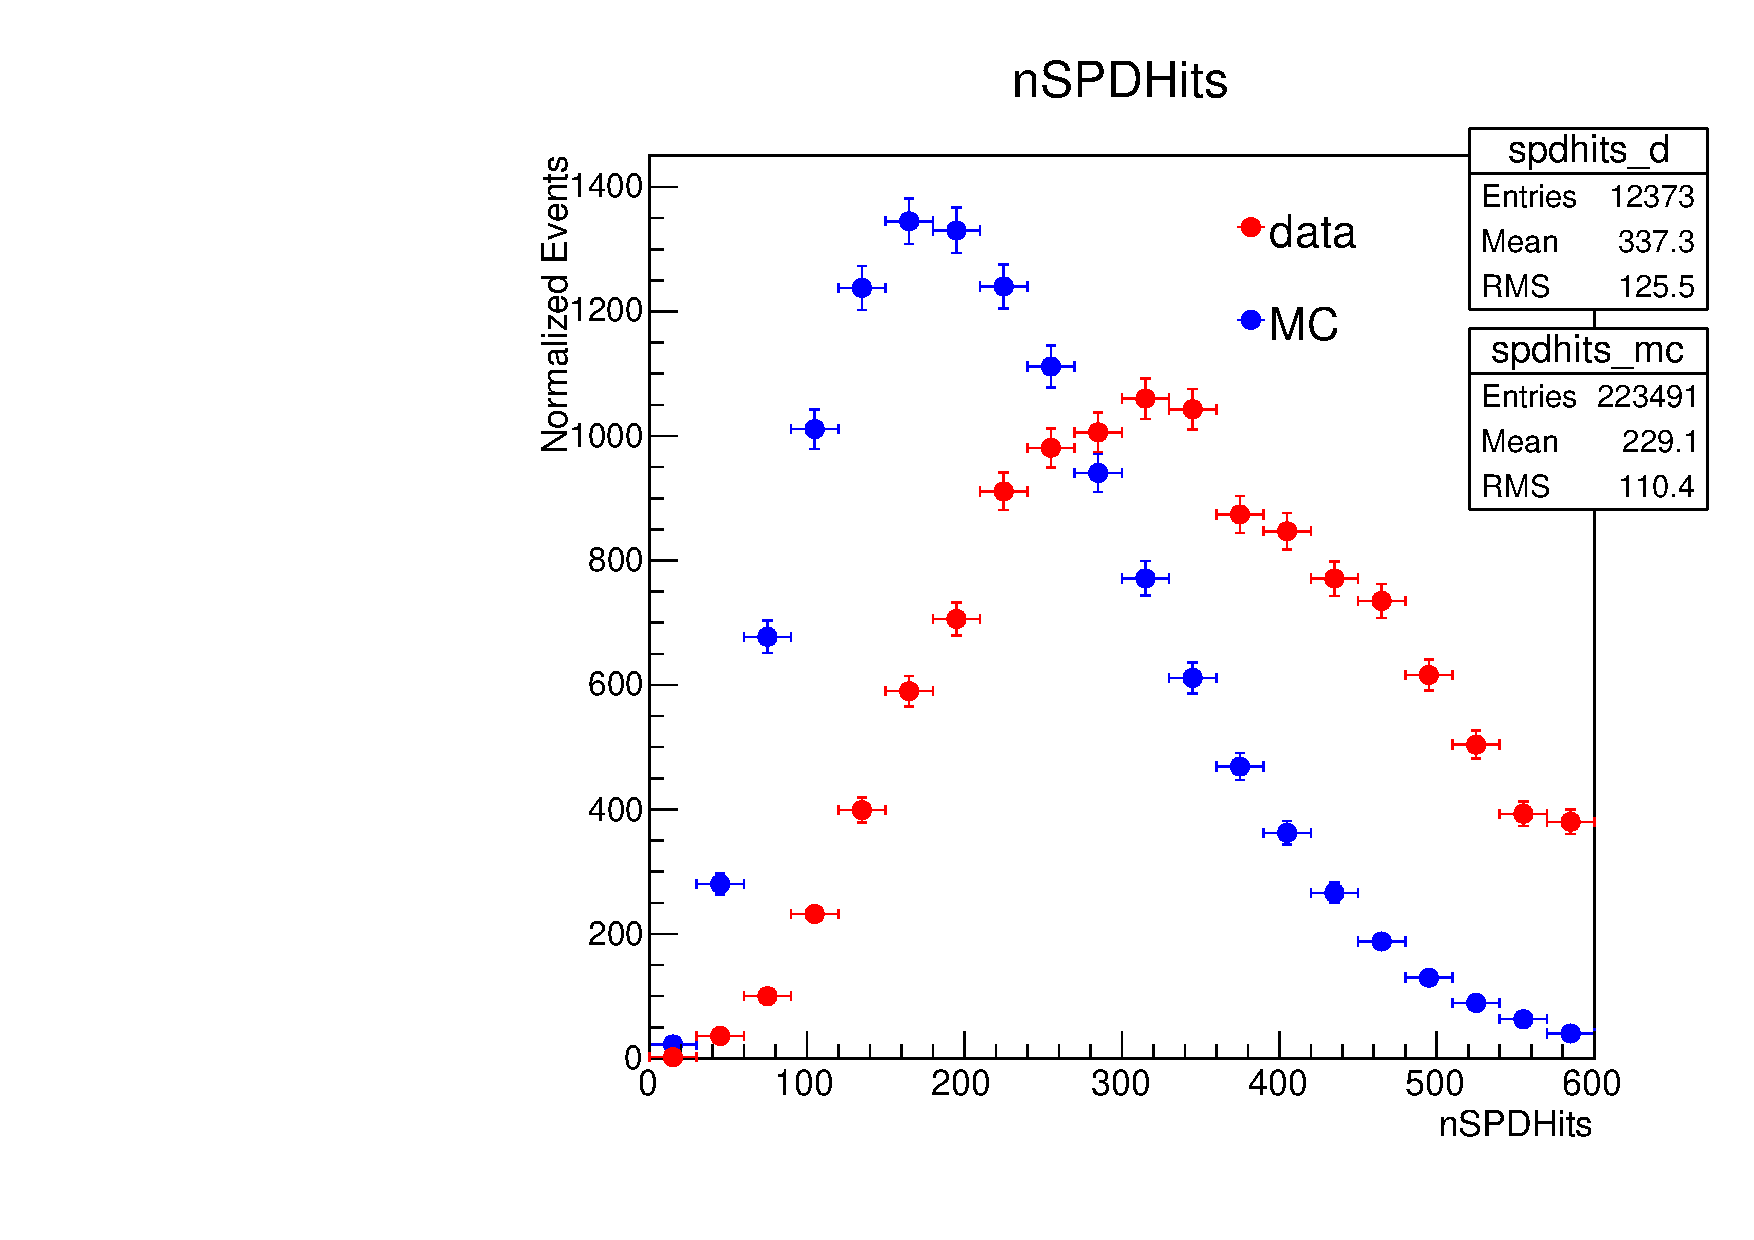
\includegraphics[width=0.48\linewidth]{MC/SPDHits_RD_MC12_BDT1_BDT2_sWeight.pdf}\put(-115,-4){(a)}
    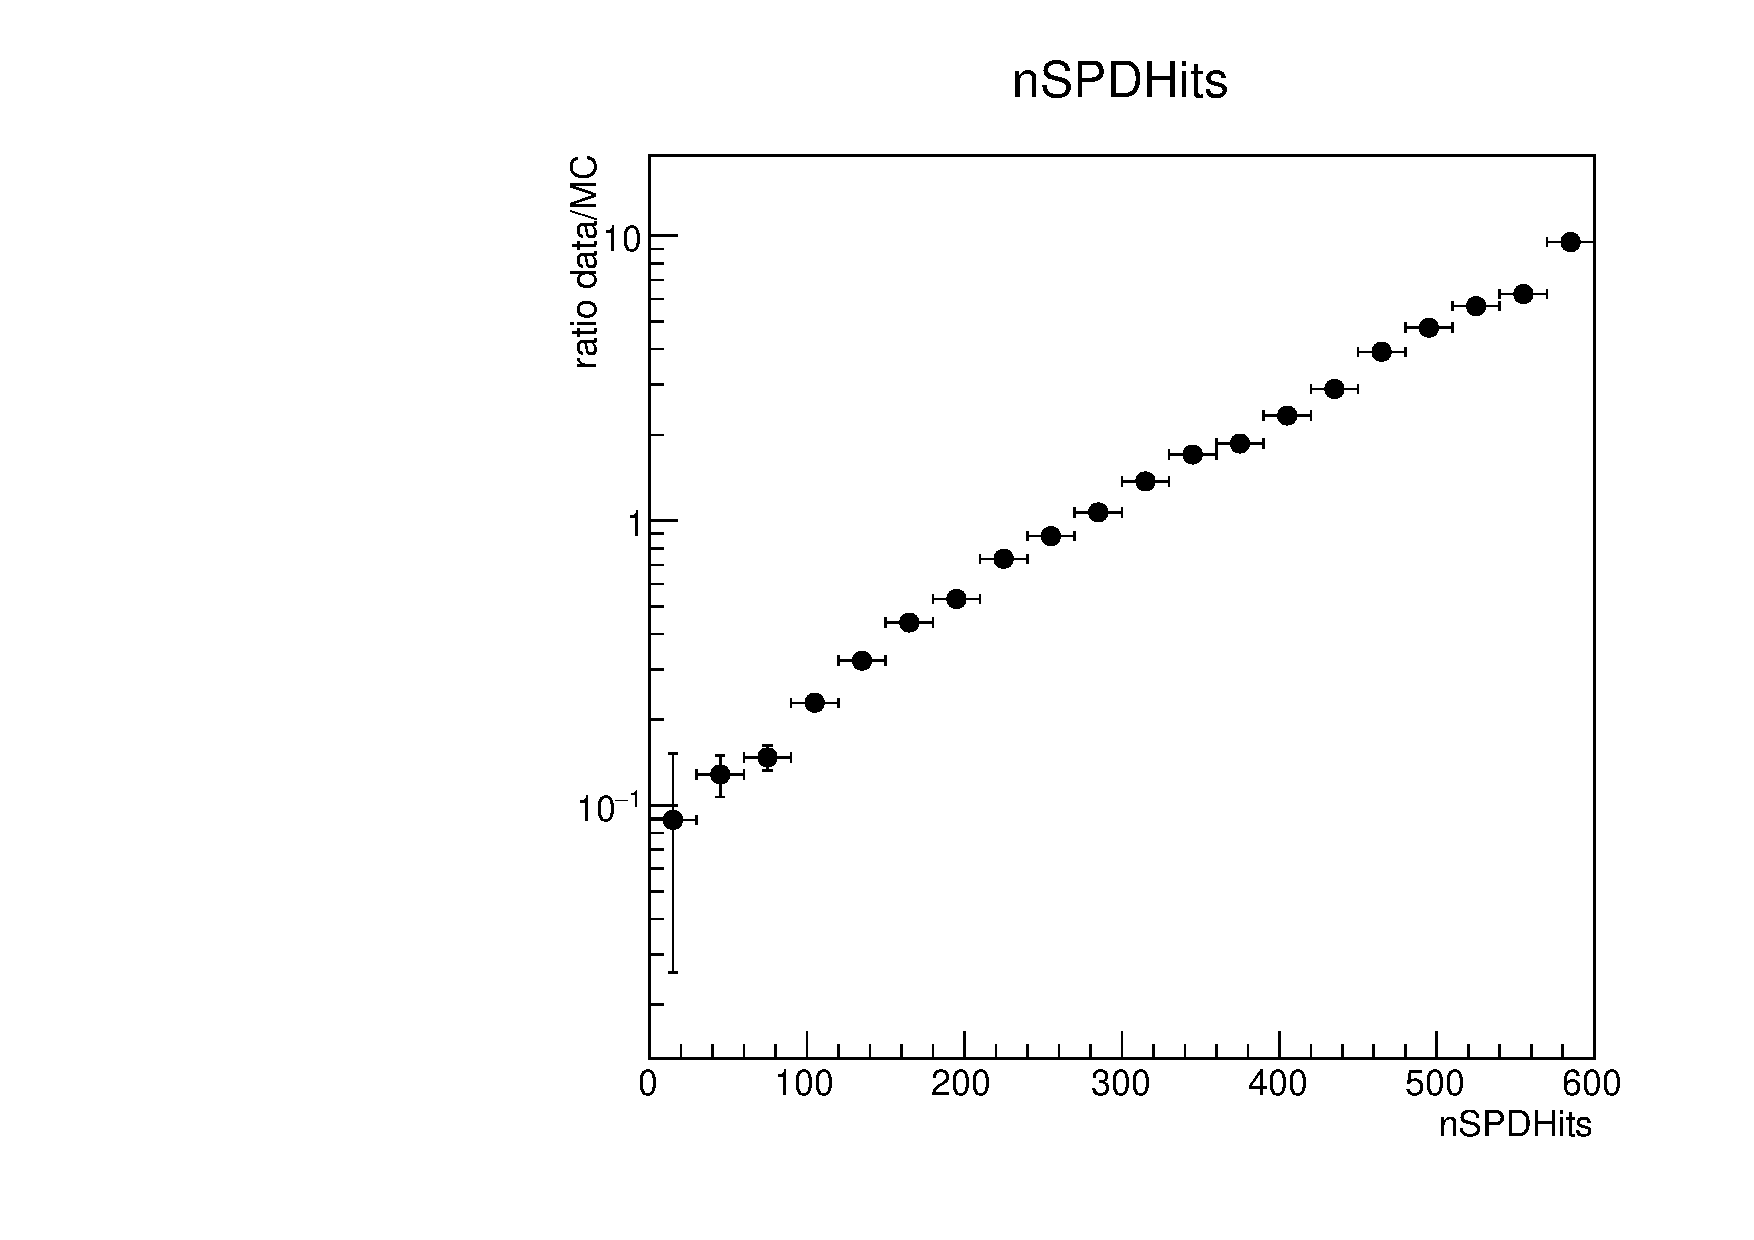
\includegraphics[width=0.48\linewidth]{MC/SPDHits_RD_MC12_BDT1_BDT2_sWeight_ratio.pdf}\put(-115,-4){(b)}
  \end{center}
  \caption{
   (a) The distribution of the number of hits in the SPD for $\Bs\to\jpsi(e^{+}e^{-})\phi$ data and MC in 2012. (b) The ratio between data and MC distributions in depends on the number of hits on the SPD. The ratio distribution is in logarithmic scale.
}
  \label{fig:nSPDHits}
\end{figure}


\subsubsection{Correction of the PID response}\label{subsubsec:PIDCalib}

The PID response is known to be not well simulated in the LHCb MC. Therefore, instead of applying the cut on the PID variables calculated in the MC, events are reweighted using PID efficiency tables. The {\tt Urania/PIDCalib} package version {\tt v4r0} is used to build PID efficiency tables for all final state particle types, $K^{\pm}$ and $e^{\pm}$. The PID efficiencies are calculated in bins of $\eta$, $p_{T}$ and number of tracks in the event. For each MC event the total PID efficiency is calculated and used to weight the event (Fig.~\ref{fig:PIDCalib}). 
\begin{figure}[htb]
  \begin{center}
    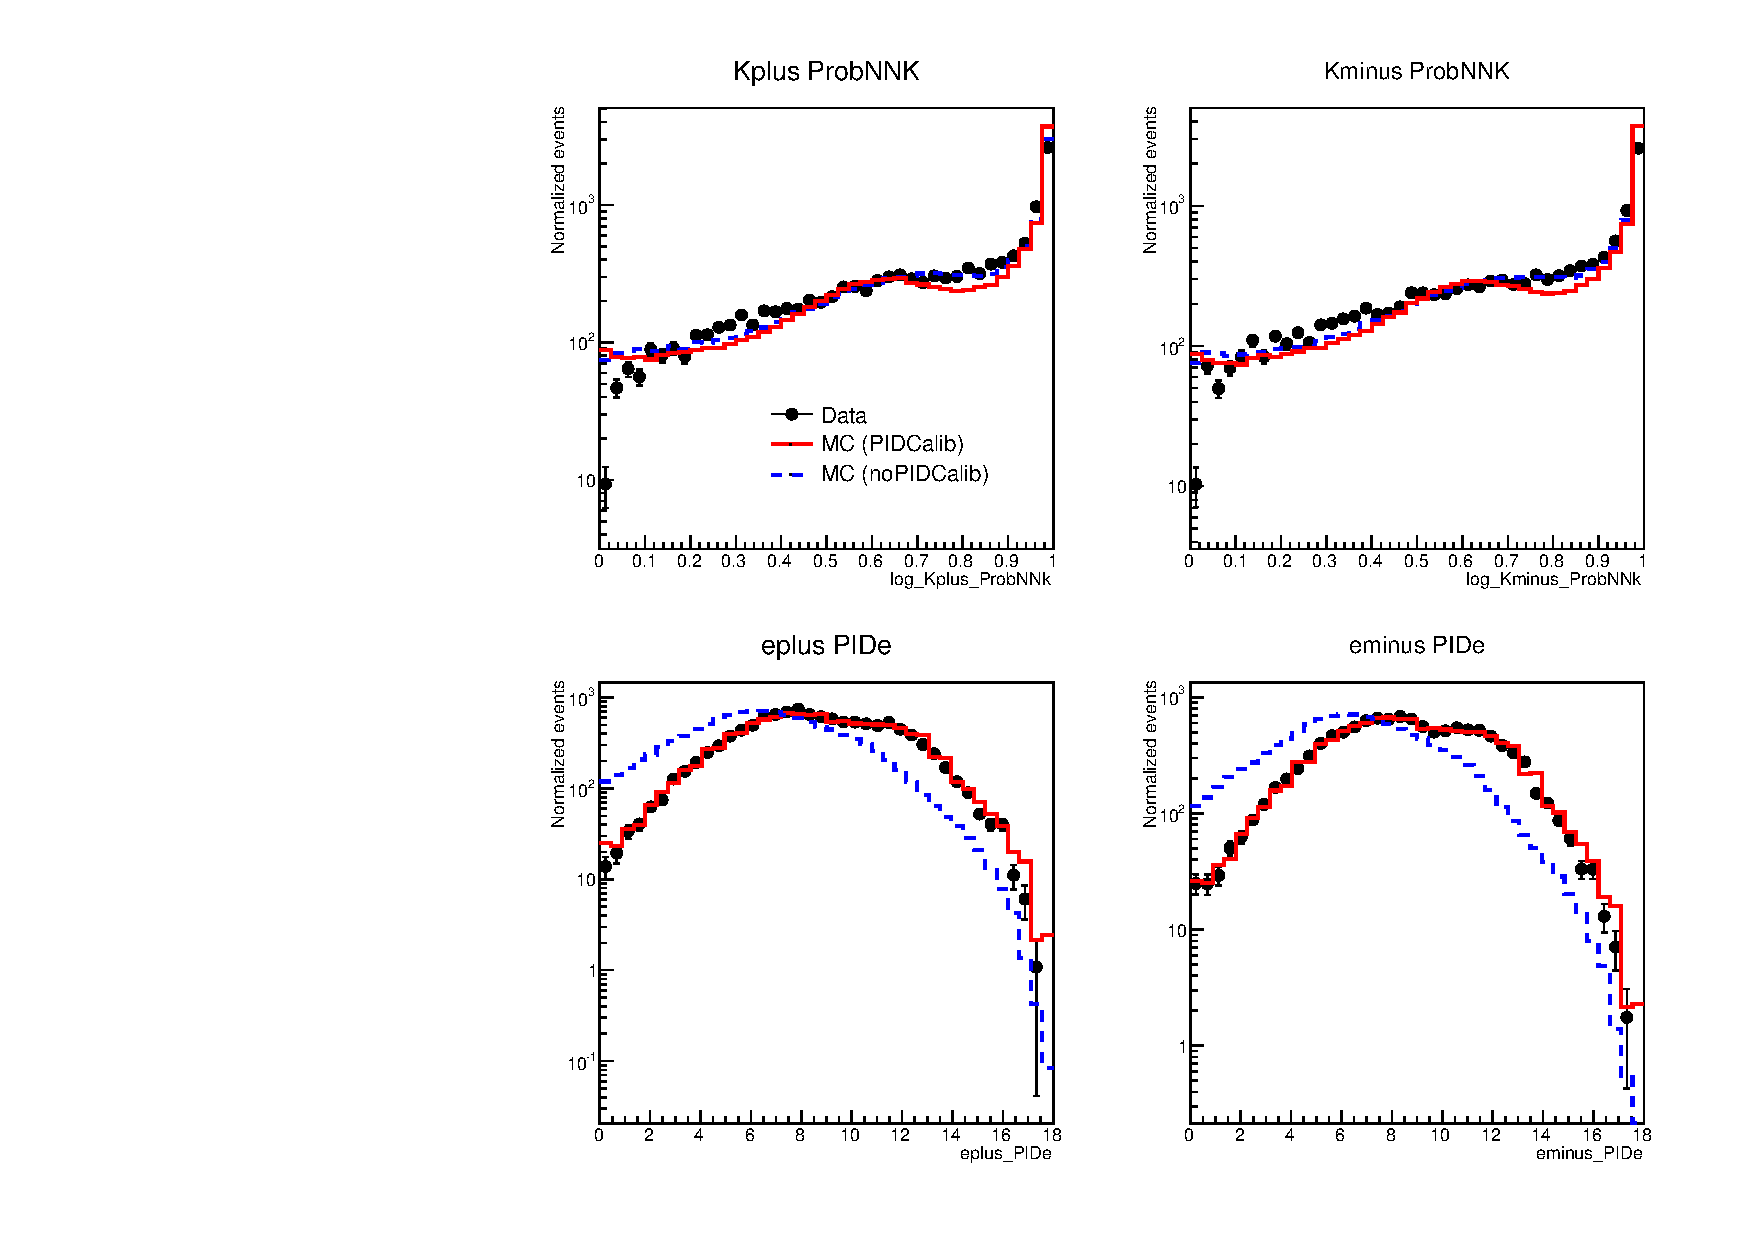
\includegraphics[width=0.8\linewidth]{Data_MC/Data_MC_PIDCalib.pdf}
  \end{center}
  \caption{
   The ProbNNK($\Kpm$) and PIDe($\epm$) distributions for $\Bs\to\jpsi(e^{+}e^{-})\phi$ in: data (black points), MC (blue dashed line) and {\tt PIDCalib} simulated data (red solid line). All distributions are in logarithmic scale.
}
  \label{fig:PIDCalib}
\end{figure}

After applying {\tt PIDCalib} algorithm the electron PIDe values for MC are in agreement with PID values for data. However, the opposite distributions obtained for ProbNN values of kaons. The kaon ProbNNK distributions for data are comparable with simulation without {\tt PIDCalib}. Thus the corrected PIDe($\epm$) and non-corrected ProbNNK($\Kpm$) variables are used in the further selection (see Sec.~\ref{subsec:BDT}).   

 \subsection{Boosted Decision Tree}\label{subsec:BDT}
  After stripping and preselection criteria (Table~\ref{tab:Selection}), the amount of background events remaining in the sample is considerable and the additional selection is required. The Boosted Decision Tree (BDT)~\cite{Hocker:2007ht} are chosen to further discriminate the signal candidates from the background. In order to have a good agreement between data and simulation, a set of kinematic variables is chosen for the BDT discriminator. In particular 12 variables are taken into consideration:
  \begin{itemize}
   \item $\pt(\jpsi)$ - the transverse momentum of the $\jpsi$ meson;
   \item $\pt(\phi)$ - the transverse momentum of the $\phi$ meson;
   \item IP$(\Bs)$ - the impact parameter of the reconstructed $\Bs$ meson with respect to the primary vertex;
   \item $\chisq_{\text{FD}}(\Bs)$ of the measured flight distance of the $\Bs$ meson;
   \item $\chisqip$ of the impact parameter of the electron and positron;
   \item $\chisqvtxndf$ of the reconstructed secondary vertex;
   \item PIDe - the difference of log-likelihood between electron and pion hypothesis for the electron and positron. In case of MC the PIDe is reweighted using {\tt PIDCalib} tool (Sec.~\ref{subsubsec:PIDCalib}) and is called PIDe$_{\text{corr}}$;
   \item ProbNNK - Neural Net (NN) log-likelihood of the kaon hypothesis for the kaons;
   \item $\chisq_{\text{DTF}}$ of the reconstructed $\Bs$ meson. 
  \end{itemize}

  The training of the BDT is done using the following samples:
  \begin{itemize}
   \item Signal: the $\Bs\to\jpsi\phi$ simulated sample is used as signal model. This sample is required to pass exactly the same stripping and preselection criteria and, furthermore, the MC truth information is used to require that the reconstructed candidate matches with the generated decay.
   \item Background: a wrong sign $\Bs\to\jpsi\phi$ data sample is used. In particular $\Bs\to\jpsi(\ep\ep)\phi(\Kp\Kp)$,  $\Bs\to\jpsi(\ep\ep)\phi(\Km\Km)$, $\Bs\to\jpsi(\en\en)\phi(\Kp\Kp)$, $\Bs\to\jpsi(\en\en)\phi(\Km\Km)$, $\Bs\to\jpsi(\ep\ep)\phi(\Kp\Km)$, $\Bs\to\jpsi(\en\en)\phi(\Kp\Km)$,  $\Bs\to\jpsi(\epem)\phi(\Kp\Kp)$ and $\Bs\to\jpsi(\epem)\phi(\Km\Km)$ events make the background sample. Also these events are required to pass all the selection steps.
  \end{itemize}
   
   The choice to use a wrong sign $\Bs\to\jpsi\phi$ data sample instead of data events taken from the sidebands of the $\Bs$ mass distribution is motivated by the fact that in this way the signal and background samples are more homogeneous. The sideband events from data ($M(\Bs)<5050$ MeV and $M(\Bs)>5550$ MeV) have also been considered to simulate the background events in the BDT training. A worse agreement between sidebands data and simulation is observed in the BDT performance description. 

  The ranking of variable importance used to train the BDT is shown in Table~\ref{tab:RankingBDT}. The BDT response is presented in Fig.~\ref{fig:BDTresponse}a. The further details on the BDT, including plots comparing the input variable distributions between signal and background, are prsented in  Appendix~\ref{sec:app:BDT}. 
   \begin{table}[hbt]
  \caption{
    The ranking of variable importance used in BDT selection.
}
    \small{
\begin{center} \begin{tabular}{ccc}
    \hline
   Rank&Variable & Importance  \\
    \hline
  1&log(ProbNNK)$(K^{+})$ & 1.149e-01 \\
  2&PIDe$(e^{-})_{\text{corr}}$ & 1.075e-01 \\
  3&log(ProbNNK)$(K^{-})$ & 1.066e-01 \\
  4&log$(\chi^{2}_{\text{IP}})(e^{-})$ & 9.723e-02 \\
  5&PIDe$(e^{+})_{\text{corr}}$ & 9.430e-02 \\
  6&log$(\chi^{2}_{\text{IP}})(e^{+})$ & 8.902e-02 \\
  7&$p_{T}(\phi)$ & 8.500e-02 \\
  8&IP$(B^{0}_{s})$ & 8.456e-02 \\
  9&$\chi^{2}_{\text{vtx}}(B^{0}_{s})$ & 7.939e-02 \\
  10&$p_{T}(J/\psi)$ & 7.595e-02 \\
  11&log$(\chi^{2}_{\text{DTF}})(B^{0}_{s})$ & 6.565e-02 \\
  12&$\chi^{2}_{\text{FD}}(B^{0}_{s})$ & 0.000e+00 \\
  \hline
    \end{tabular}\end{center}
  }
\label{tab:RankingBDT}
\end{table}

\begin{figure}[ht!]
  \begin{center}
    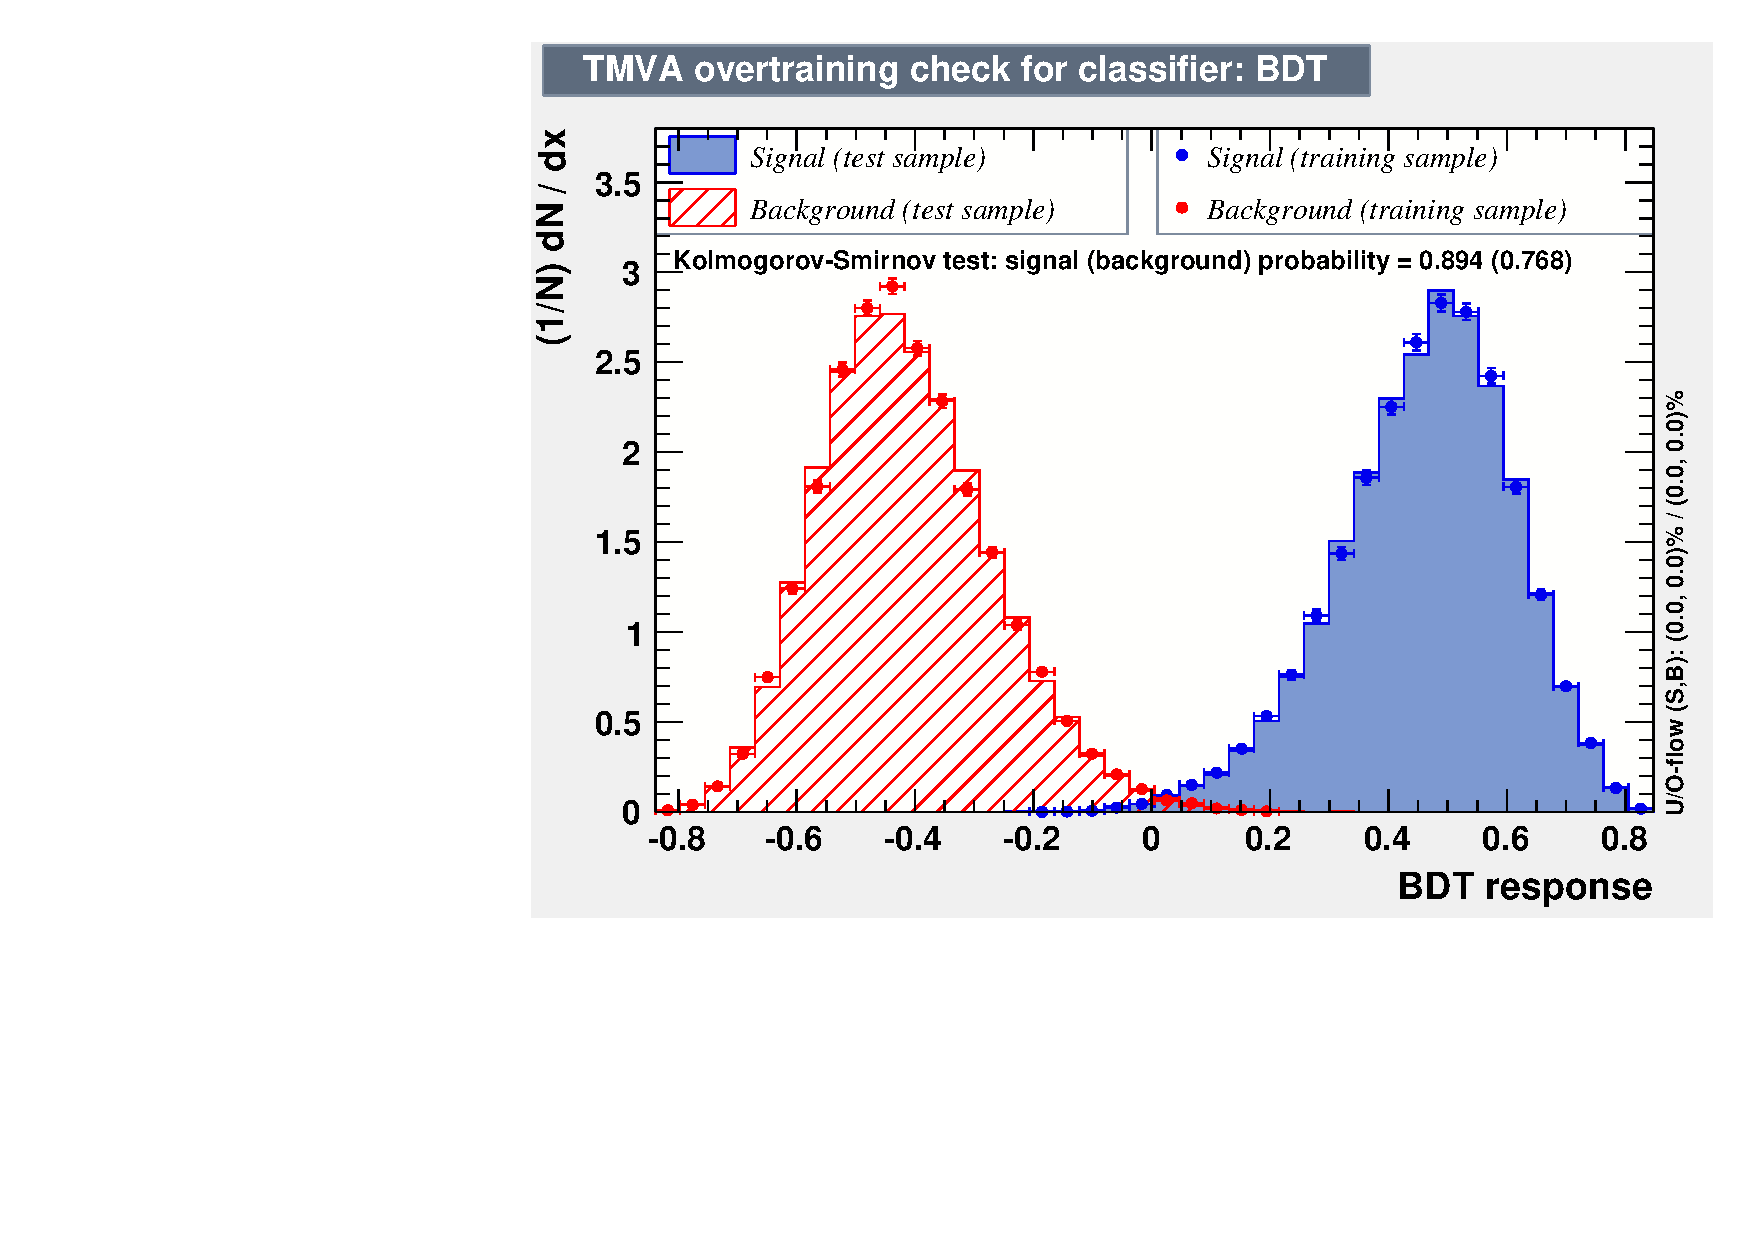
\includegraphics[width=0.49\linewidth]{BDT/BDT_response_bkgcat0_wSPDHits_trigger_RD12.pdf}\put(-115,-13){(a)}
    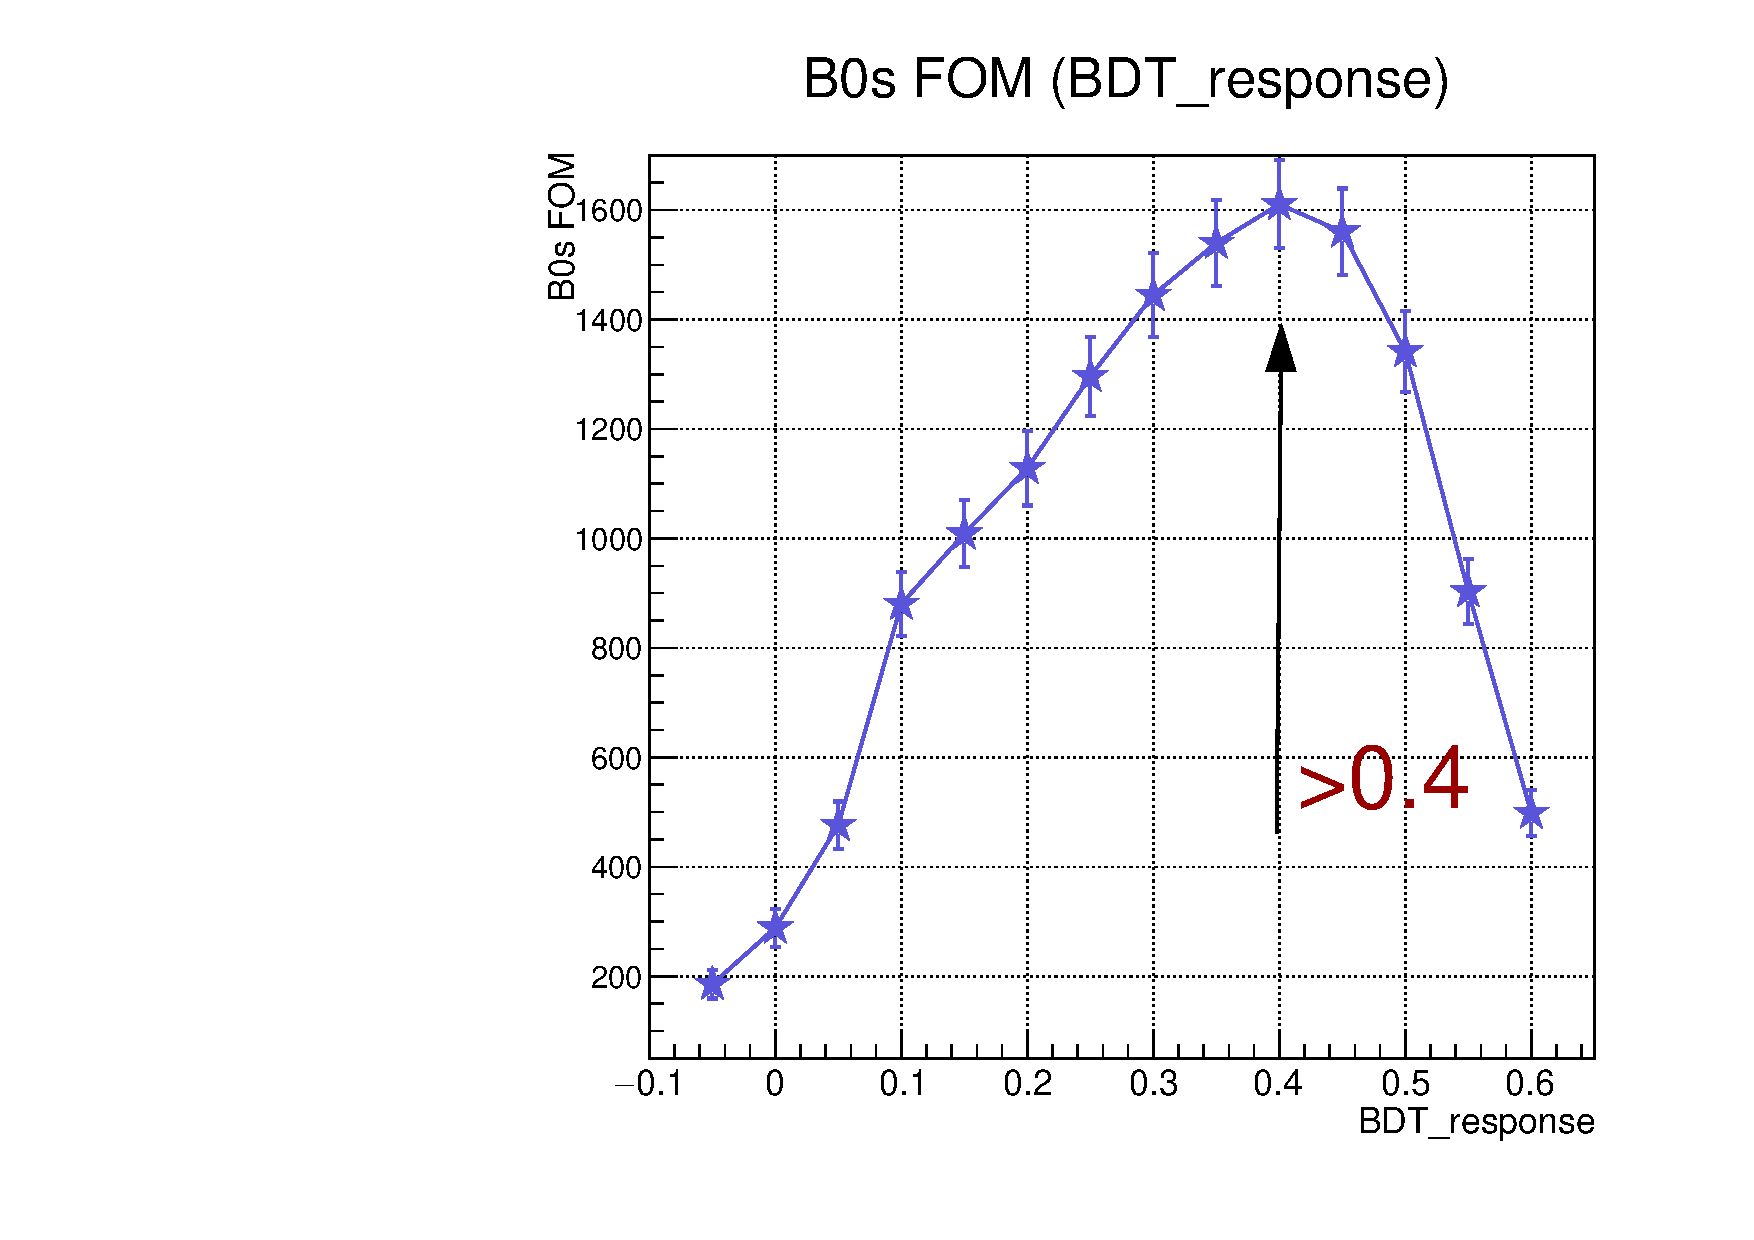
\includegraphics[width=0.41\linewidth]{BDT/FoM_BDT_response.pdf}\put(-115,-13){(b)}
  \end{center}
  \caption{
   (a) The distributions of the BDT classifier for $\Bs\to\jpsi\phi$ training samples. The signal is red hatched filled while the background is blue solid filled.  (b) The distribution of the FoM value vs. cut on the BDT response.  
}
  \label{fig:BDTresponse}
\end{figure}
  The BDT response is the combined vote of many individual decision trees. It can be used as a univariate discriminant to distinguish signal from background. To choose where to cut on the BDT response we use a figure of merit (FoM) value (Eq.~\ref{eq:FoM})~\cite{Xie:2009yz}, which is defined as an effective size of the signal defined using the signal sWeight $w_i$: 
  \begin{equation}\label{eq:FoM}
   FoM=\frac{(\sum^{N}_{i=1}w_i)^{2}}{\sum^{N}_{i=1}w^{2}_{i}}.
  \end{equation}
  The sWeight is calculated using the sPlot technique~\cite{Pivk:2004ty} of statistical separation of signal events from background. The Fig.~\ref{fig:BDTresponse}b presents the dependence of the $\Bs$ FoM value on the BDT response. The optimal cut which maximises the signal size of selected events with BDT response is chosen larger than 0.4. 
  
  \subsection{Peaking background}\label{subsec:PeakBkg}

%   Two possible source of a background that peaks under the signal $\Bs$ peak are $\Bz\to\jpsi\Kstar$ decays, where a $\pi$ from the $\Kstar\to K\pi$ decay has been misidentified as a $K$, and $\Lb\to\jpsi(\epem) pK$ decays, where the $p$ has been misidentifiedas a $K$. To estimate the expected amount of these background the $\Bz\to\jpsi\Kstar$ and $\Lb\to\jpsi pK$ are reconstructed as the analyzed decay. The comparison of transverse momentum and mass distributions between the simulated signal channel and the background simulation is presented in Fig.~\ref{fig:Bs_MM_MC12}. The number of simulated signal events is 557 908 with 2 877 $\Bz\to\jpsi\Kstar$ events and 6 323 $\Lb\to\jpsi pK$ events passing through the selection.
  
  
  The possible source of a background that peaks under the signal $\Bs$ mass distribution is considered as the $\Lb\to\jpsi(\epem) pK$ decay, where a proton may be misidentified as a kaon. To estimate the expected background amount, the $\Lb\to\jpsi pK$ is reconstructed in the similar scheme as the analyzed decay.  
  \begin{figure}[hbt]
  \begin{center}
    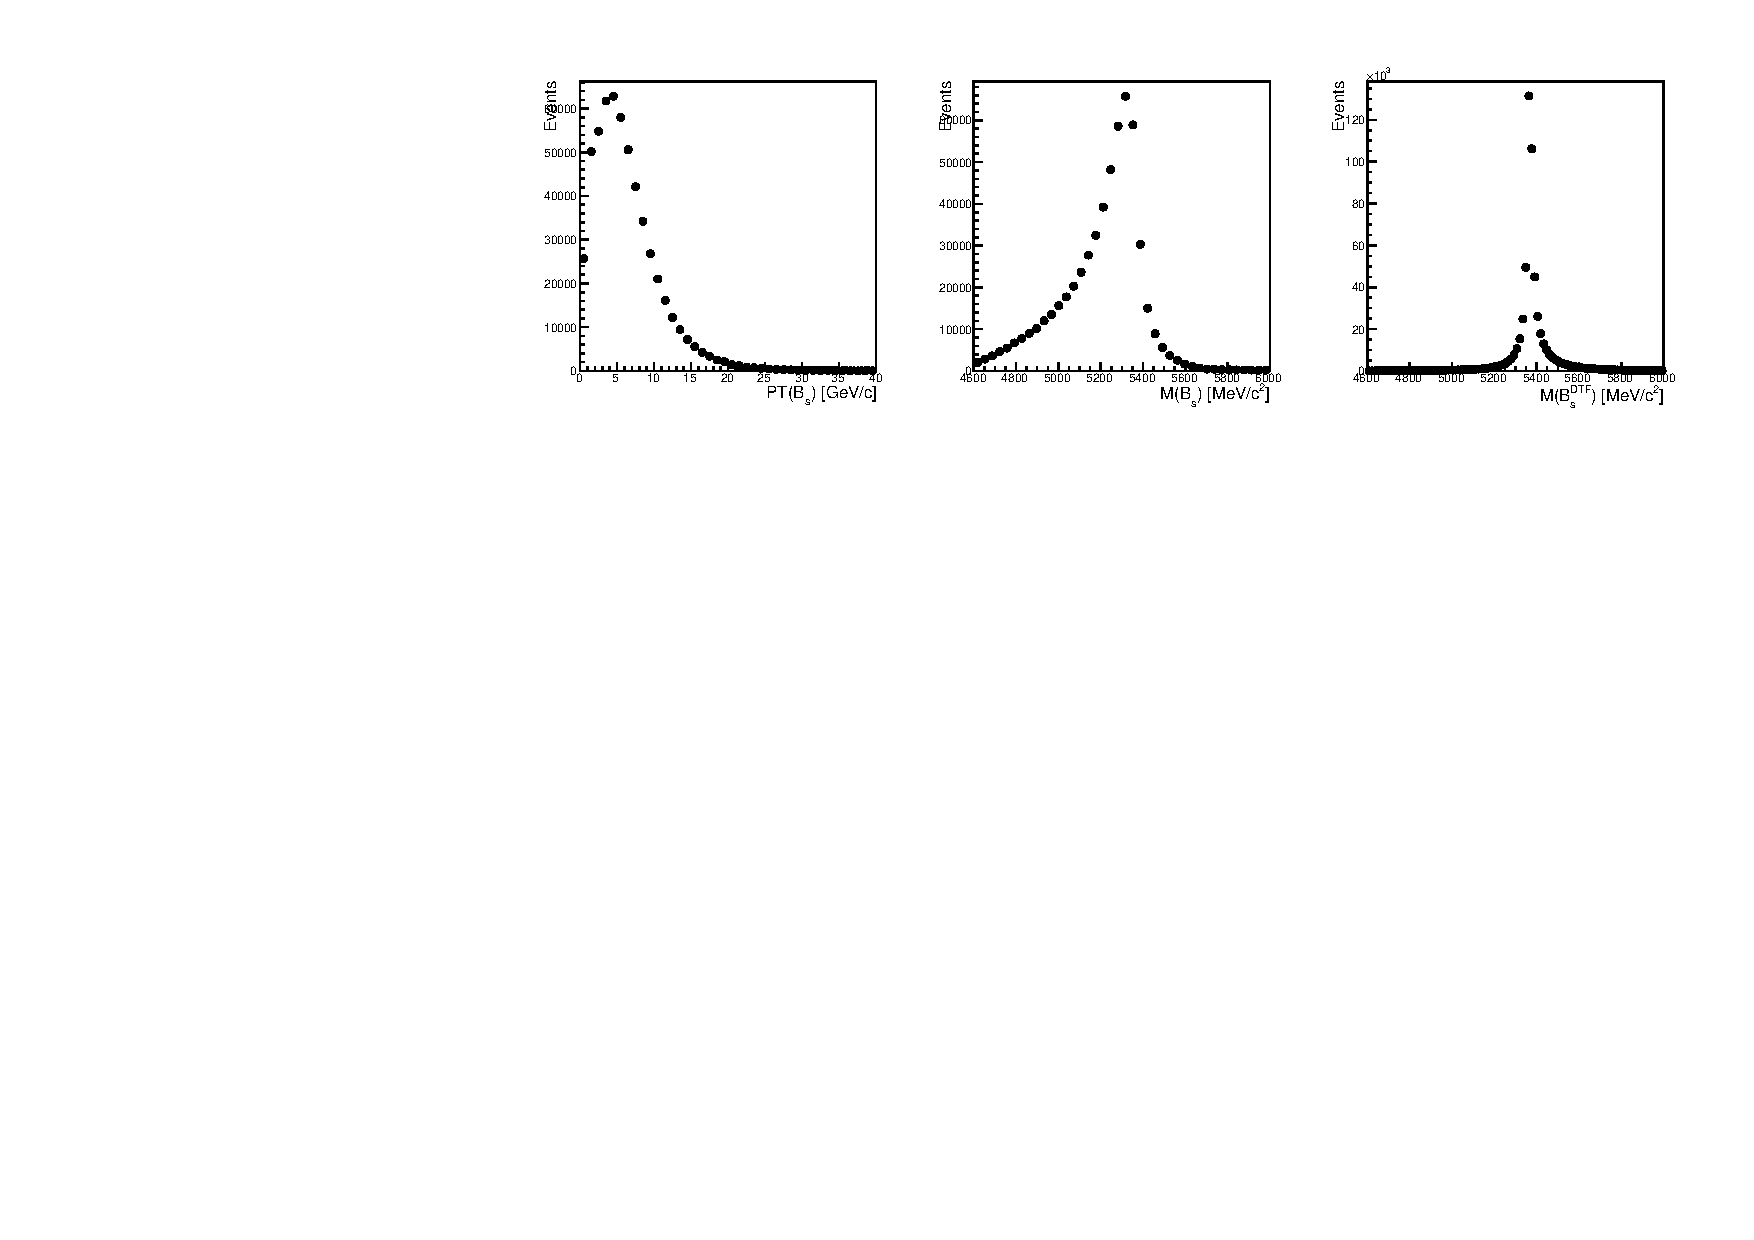
\includegraphics[width=1\linewidth]{Bkg_Bspeak/Bs_MM_MC12.pdf} \\
    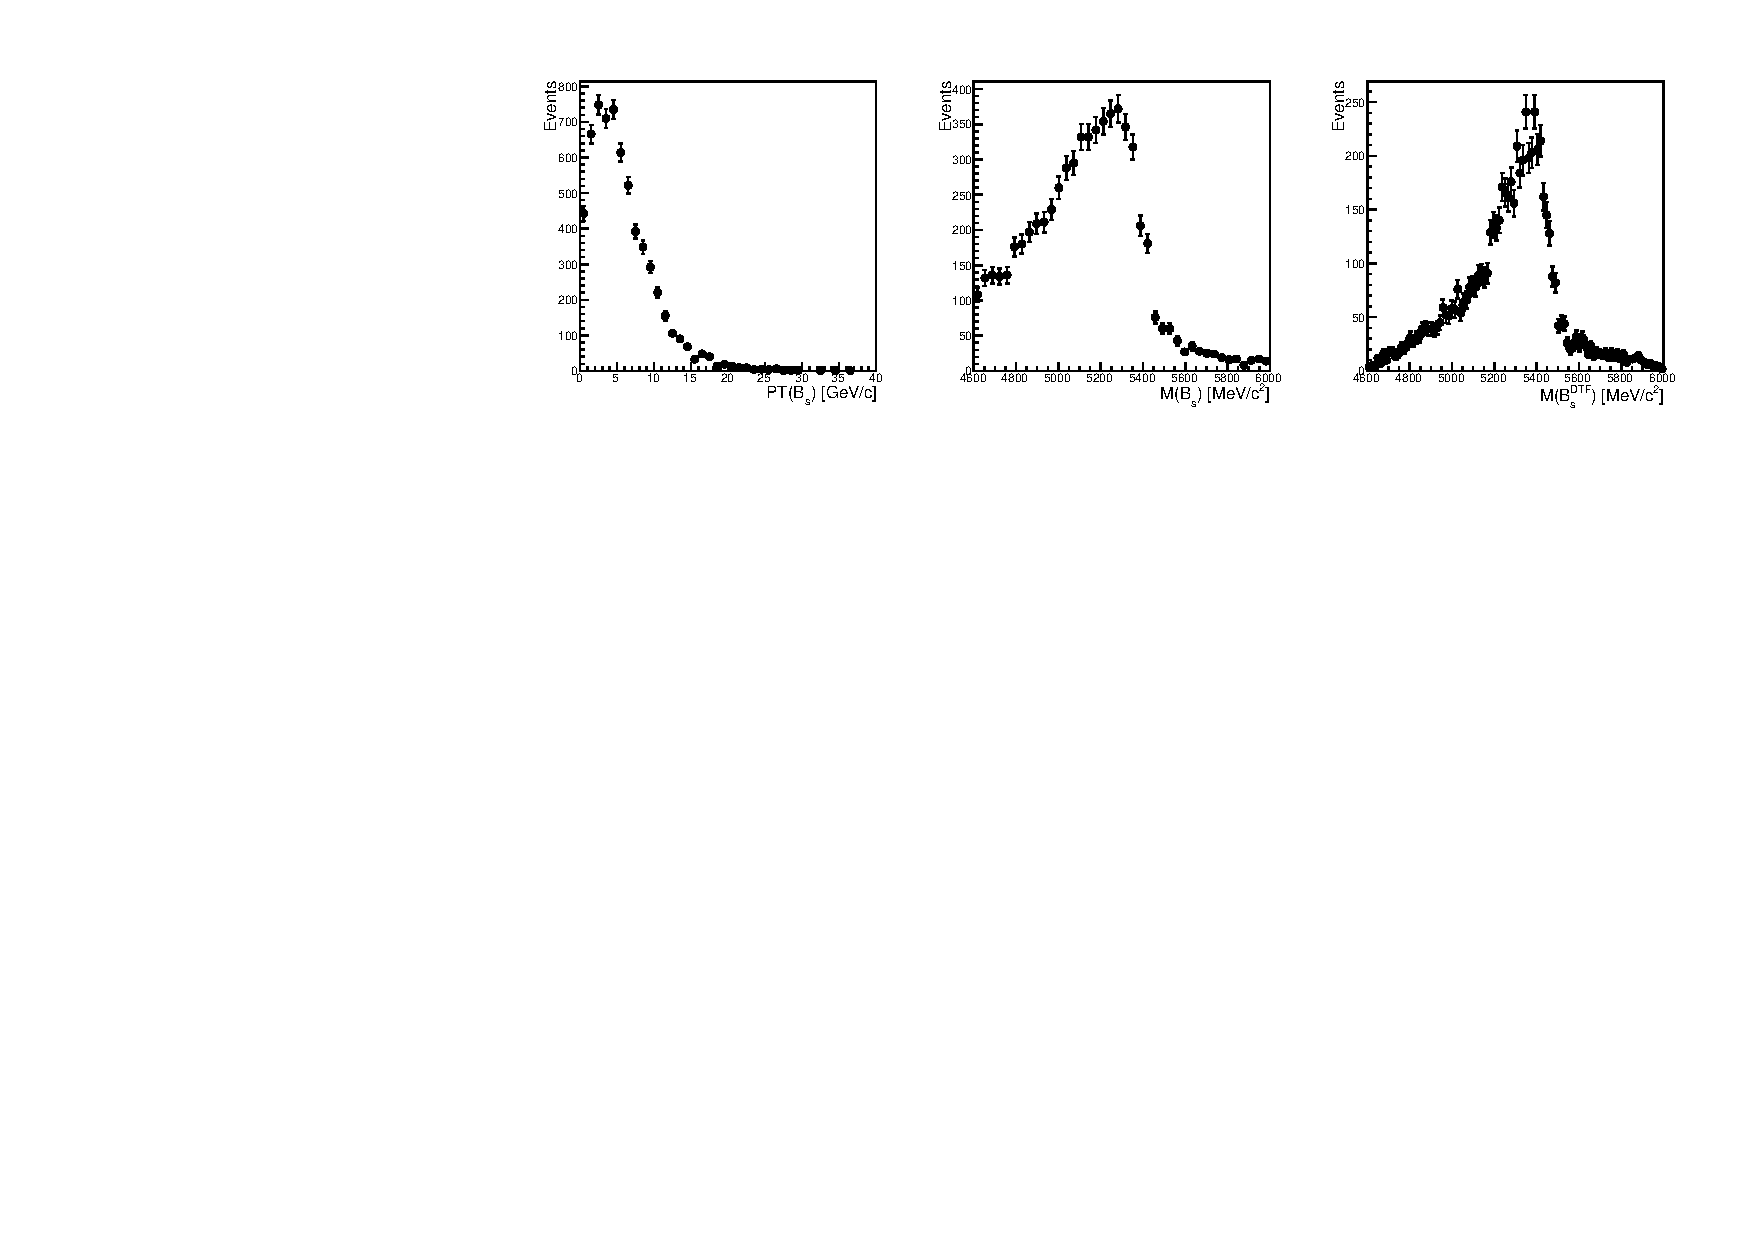
\includegraphics[width=1\linewidth]{Bkg_Bspeak/Bs_Lb2JpsipK_MM_MC12.pdf}
  \end{center}
  \caption{
   The transverse momentum and mass distributions of signal $\Bs\to\jpsi\phi$ events (top) and $\Lb\to\jpsi pK$ events reconstructed as $\Bs\to\jpsi\phi$ decay (bottom). The distributions correspond to 2012 simulated sample.   
}
  \label{fig:Bs_MM_MC12}
\end{figure}
  The transverse momentum and mass distributions of the simulated signal $\Bs\to\jpsi\phi$ and background $\Lb\to\jpsi pK$ channels are presented in Fig.~\ref{fig:Bs_MM_MC12}. The number of simulated signal events is 557 908 with 6 323 $\Lb\to\jpsi pK$ events passing through the selection.
  
To reduce the contribution of $\Lb\to\jpsi pK$ decay, a second BDT is trained using the following samples:
 \begin{itemize}
   \item Signal: the simulated $\Bs\to\jpsi\phi$ sample is used as the signal model. This sample is required to pass exactly the same stripping and preselection criteria as described in Sec.~\ref{subsec:EvtSel}. Furthermore the MC truth information is used to require that the reconstructed candidate matches with the generated decay.
   \item Background: the simulated $\Lb\to\jpsi pK$ sample reconstructed as a signal channel is used. Also these events are required to pass all the selection steps.
  \end{itemize}
 A set of 13 kinematic variables is taken as an input for the BDT discriminator, where 12 variables are the same as used in the first BDT training (Sec.~\ref{subsec:BDT}). The additional variable is the log-likelihood of the proton hypothesis for a kaon and it is the variable with the largest importance for the BDT technique. The ranking of the variable importance used to train the BDT is shown in Table~\ref{tab:RankingBDT2}. The plots comparing the input variable distributions between signal and background are shown in Appendix~\ref{sec:app:BDT}.
 
 \begin{table}[htb]
  \caption{
    The ranking of the variable importance used in peaking background BDT selection.
}
    \small{
\begin{center} \begin{tabular}{ccc}
    \hline
   Rank&Variable & Importance  \\
    \hline
  1&log(ProbNNp)($K^{+}$) & 1.503e-01 \\
  2&log(ProbNNK)$(K^{-})$ & 1.413e-01 \\
  3&$\chi^{2}_{\text{vtx}}(B^{0}_{s})$ & 1.338e-01 \\
  4&log$(\chi^{2}_{\text{IP}})(e^{+})$ & 1.316e-01 \\
  5&log$(\chi^{2}_{\text{IP}})(e^{-})$ & 9.461e-02 \\
  6&log(ProbNNK)$(K^{+})$ & 8.547e-02 \\
  7&$p_{T}(J/\psi)$ & 8.475e-02 \\
  8&$p_{T}(\phi)$ & 7.417e-02 \\
  9&PIDe$(e^{-})_{\text{corr}}$ & 3.015e-02 \\
  10&IP$(B^{0}_{s})$ & 2.547e-02 \\
  11&PIDe$(e^{+})_{\text{corr}}$ & 2.455e-02 \\
  12&log$(\chi^{2}_{\text{DTF}})(B^{0}_{s})$ & 2.387e-02 \\
  13&$\chi^{2}_{\text{FD}}(B^{0}_{s})$ & 0.000e+00 \\
  \hline
    \end{tabular}\end{center}
  }
\label{tab:RankingBDT2}
\end{table}

In the case of second BDT training, the BDT classifier distribution doesn't have a good separation of signal from background since the variables for trained samples have similar distributions and values (Fig.~\ref{fig:BDTLbresponse}a). For these reasons, it is not possible to build a FoM based on sWeights. Therefore a new figure of merit (FoM2) is used to define a selection criterium:
\begin{equation}\label{eq:FoM2}
   FoM2=\frac{S}{\sqrt{S+B1+B2}},
  \end{equation}
where $S$, $B1$ and $B2$ are the number of the signal and two types of the background events, respectively. The $B1$ and $B2$ background events are defined by the exponential and Gaussian functions, respectively. A two Crystal Ball functions with a common mean determine the signal shape. The mass fits are shown in Sec.~\ref{sec:BsFit}. The dependence of the FoM2 value on BDT response cut is shown in Fig.~\ref{fig:BDTLbresponse}b. All FoM values are consistent to each other within the limits of uncertainty. The optimal cut of $>$0.15 is chosen to select the final data sample. 
\begin{figure}[ht!]
  \begin{center}
    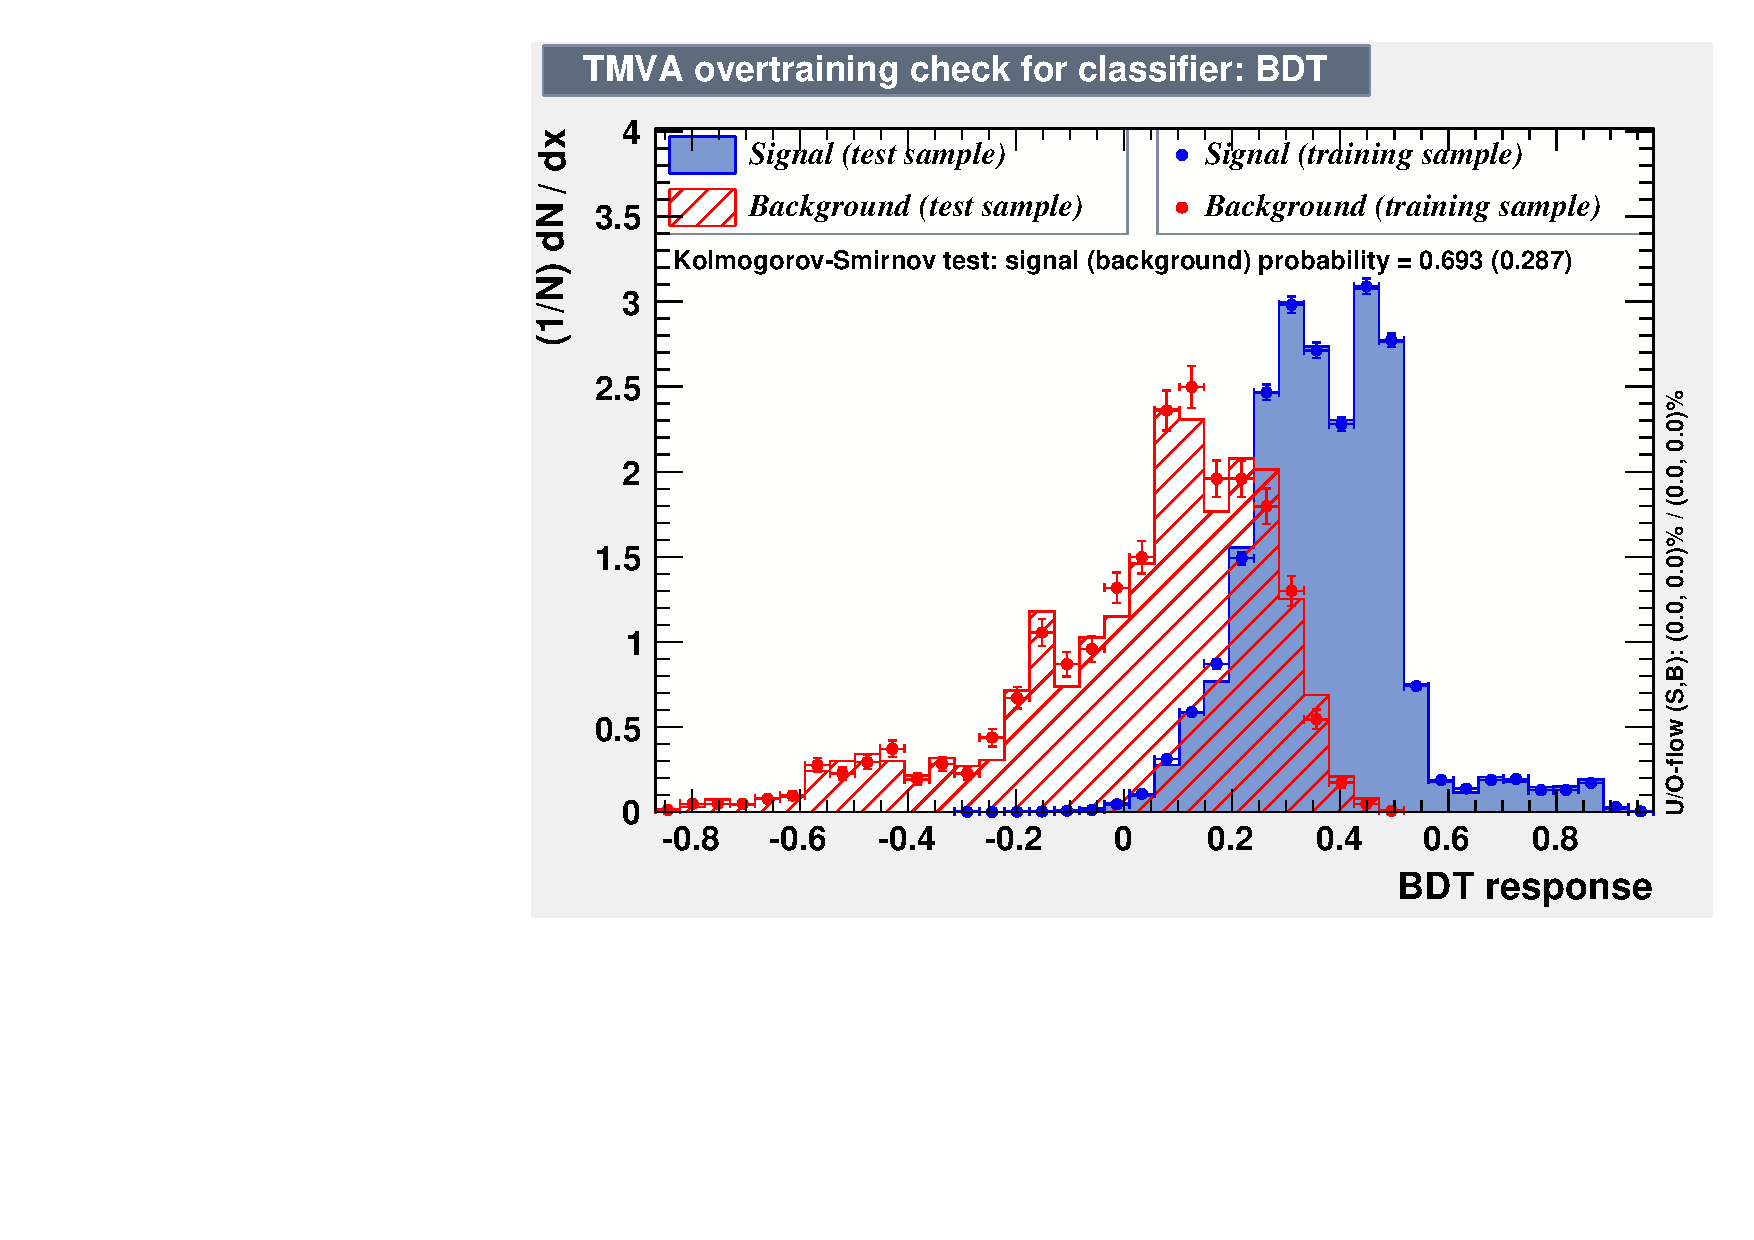
\includegraphics[width=0.49\linewidth]{BDT/BDTLb_response_bkgcat0_wSPDHits_trigger_RD12.pdf}\put(-115,-13){(a)}
    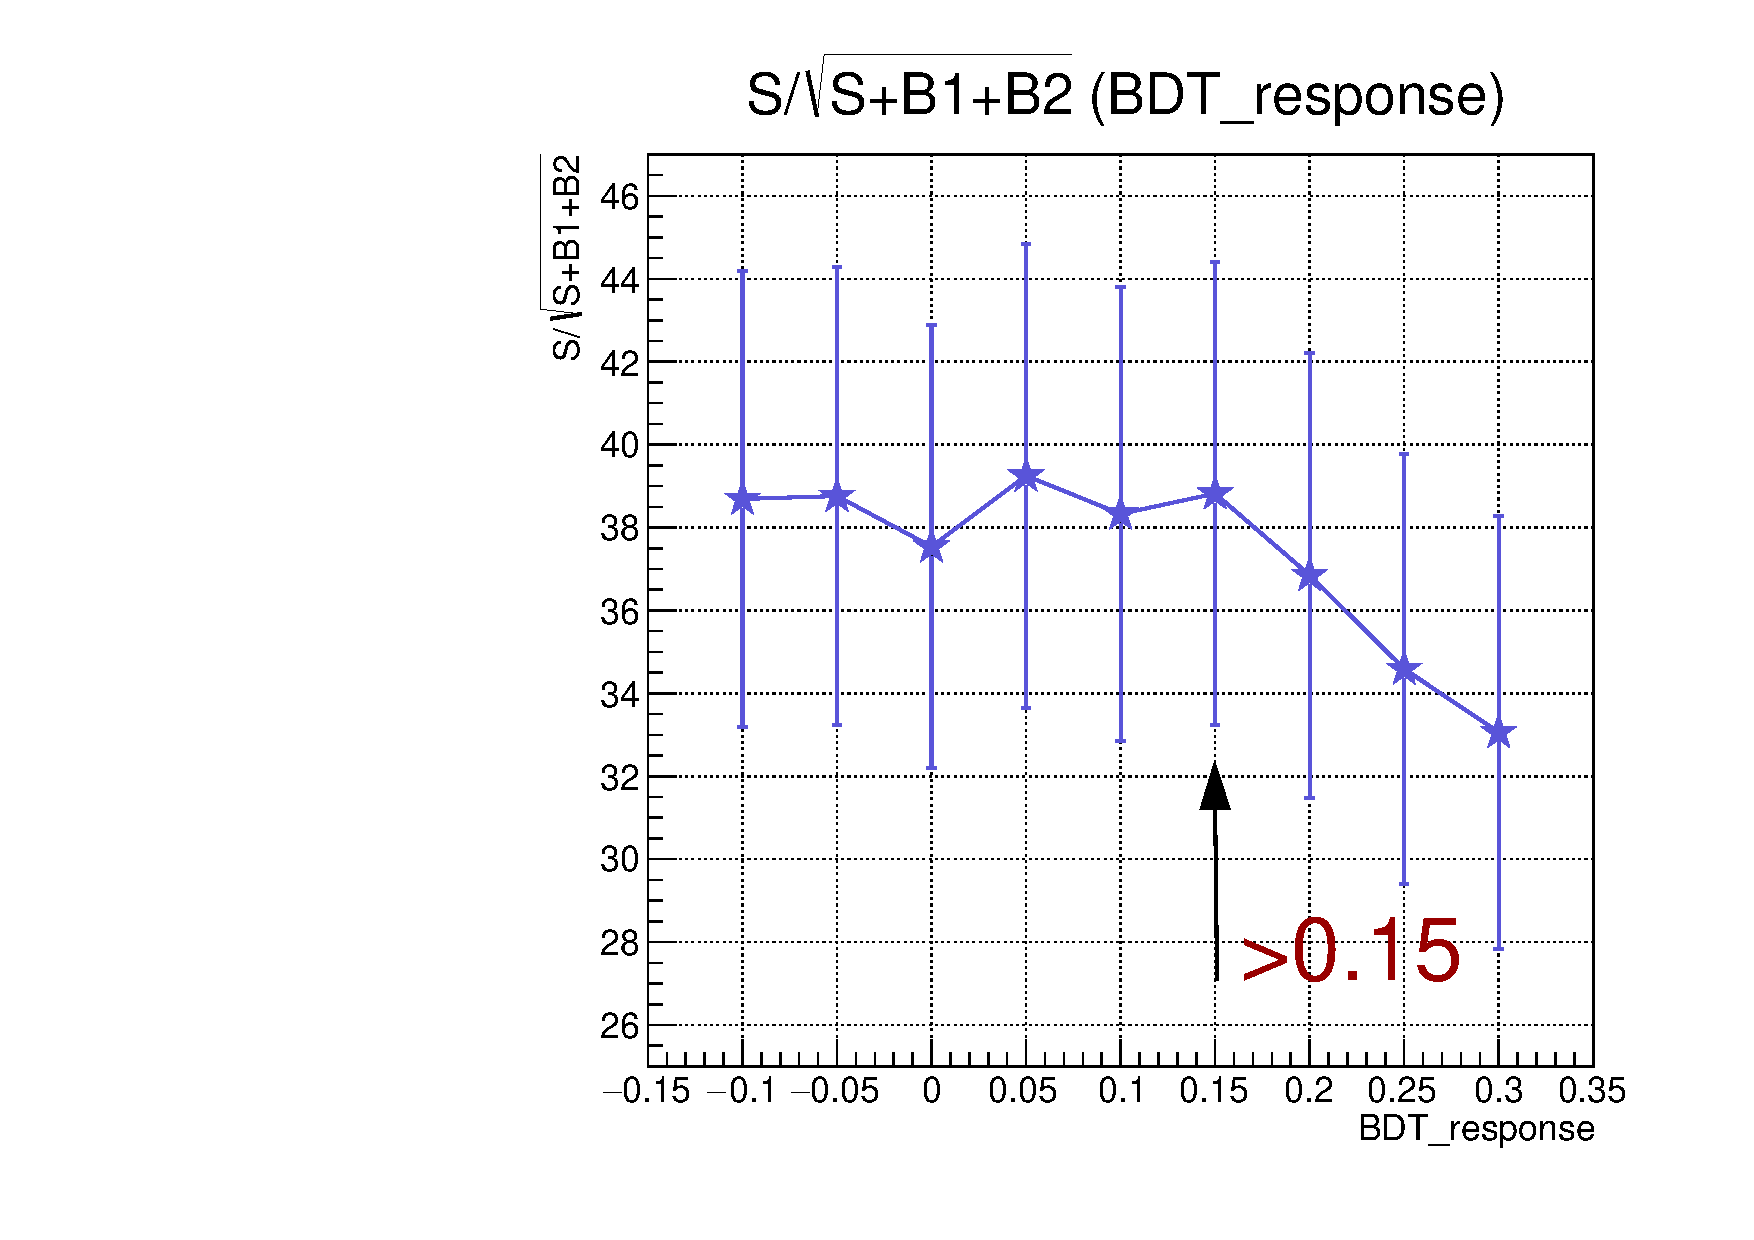
\includegraphics[width=0.4\linewidth]{BDT/FoM_BDTLb_response.pdf}\put(-115,-13){(b)}
  \end{center}
  \caption{
   (a) The distributions of the peaking background BDT classifier for $\Bs\to\jpsi\phi$ training samples. The signal is red hatched filled while background is blue solid filled. (b) The distribution of the FoM2 value in depends on the BDT response cut.  
}
  \label{fig:BDTLbresponse}
\end{figure}

After applying this cut the number of the $\Lb\to\jpsi pK$ events is in the MC sample has decreased by 44.5$\%$. This corresponds to decrease the number of $\Bs\to\jpsi\phi$ candidates by 4.2$\%$ for the data sample.   
\clearpage
  
\section{Mass fit}\label{sec:BsFit}

The $\jpsi$ and $\phi$ mass fit result after all selection steps (Sec.~\ref{subsec:EvtSel}-\ref{subsec:PeakBkg}) using 3~$\invfb$ data sample is presented in Fig.~\ref{fig:JpsiPhimass}. The $\jpsi$ mass fit is performed using a sum of two Crystal Ball functions with a common mean for the signal and a polynomial function for the background events. In case of the $\phi$ meson, as a mass model a sum of double Gaussian and Voigtian functions~\cite{OLIVERO1977233} is used with a common mean for the signal candidates and a Chebychev polynomial for the background. The signal and the background yields from the fits to the two mesons are performed separately for 2011 and 2012 and the results are shown in Table~\ref{tab:JpsiPhiTable}.
\begin{figure}[htb]
  \begin{center}
    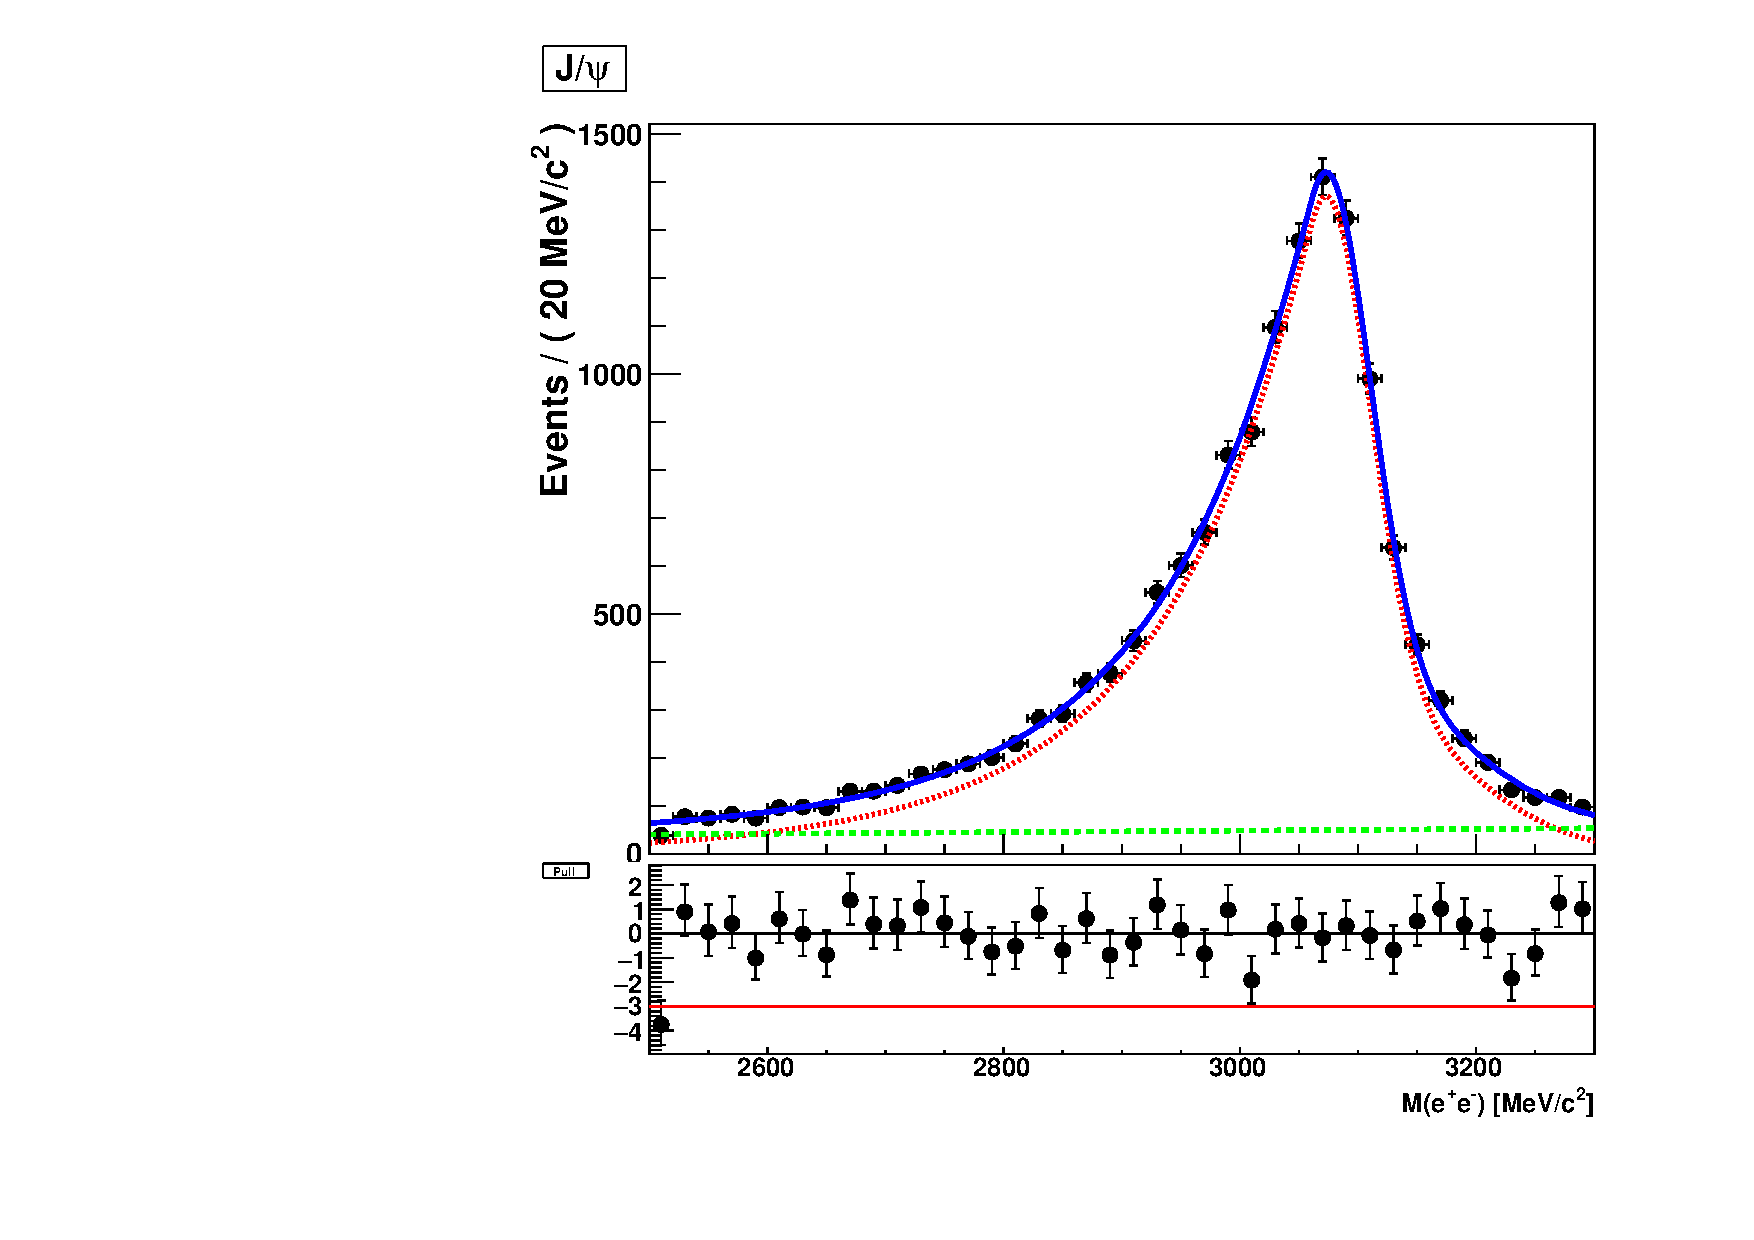
\includegraphics[width=0.49\linewidth]{RDfull_BDT1_BDT2_sWeight/mdau1.pdf}\put(-115,-4){(a)}
    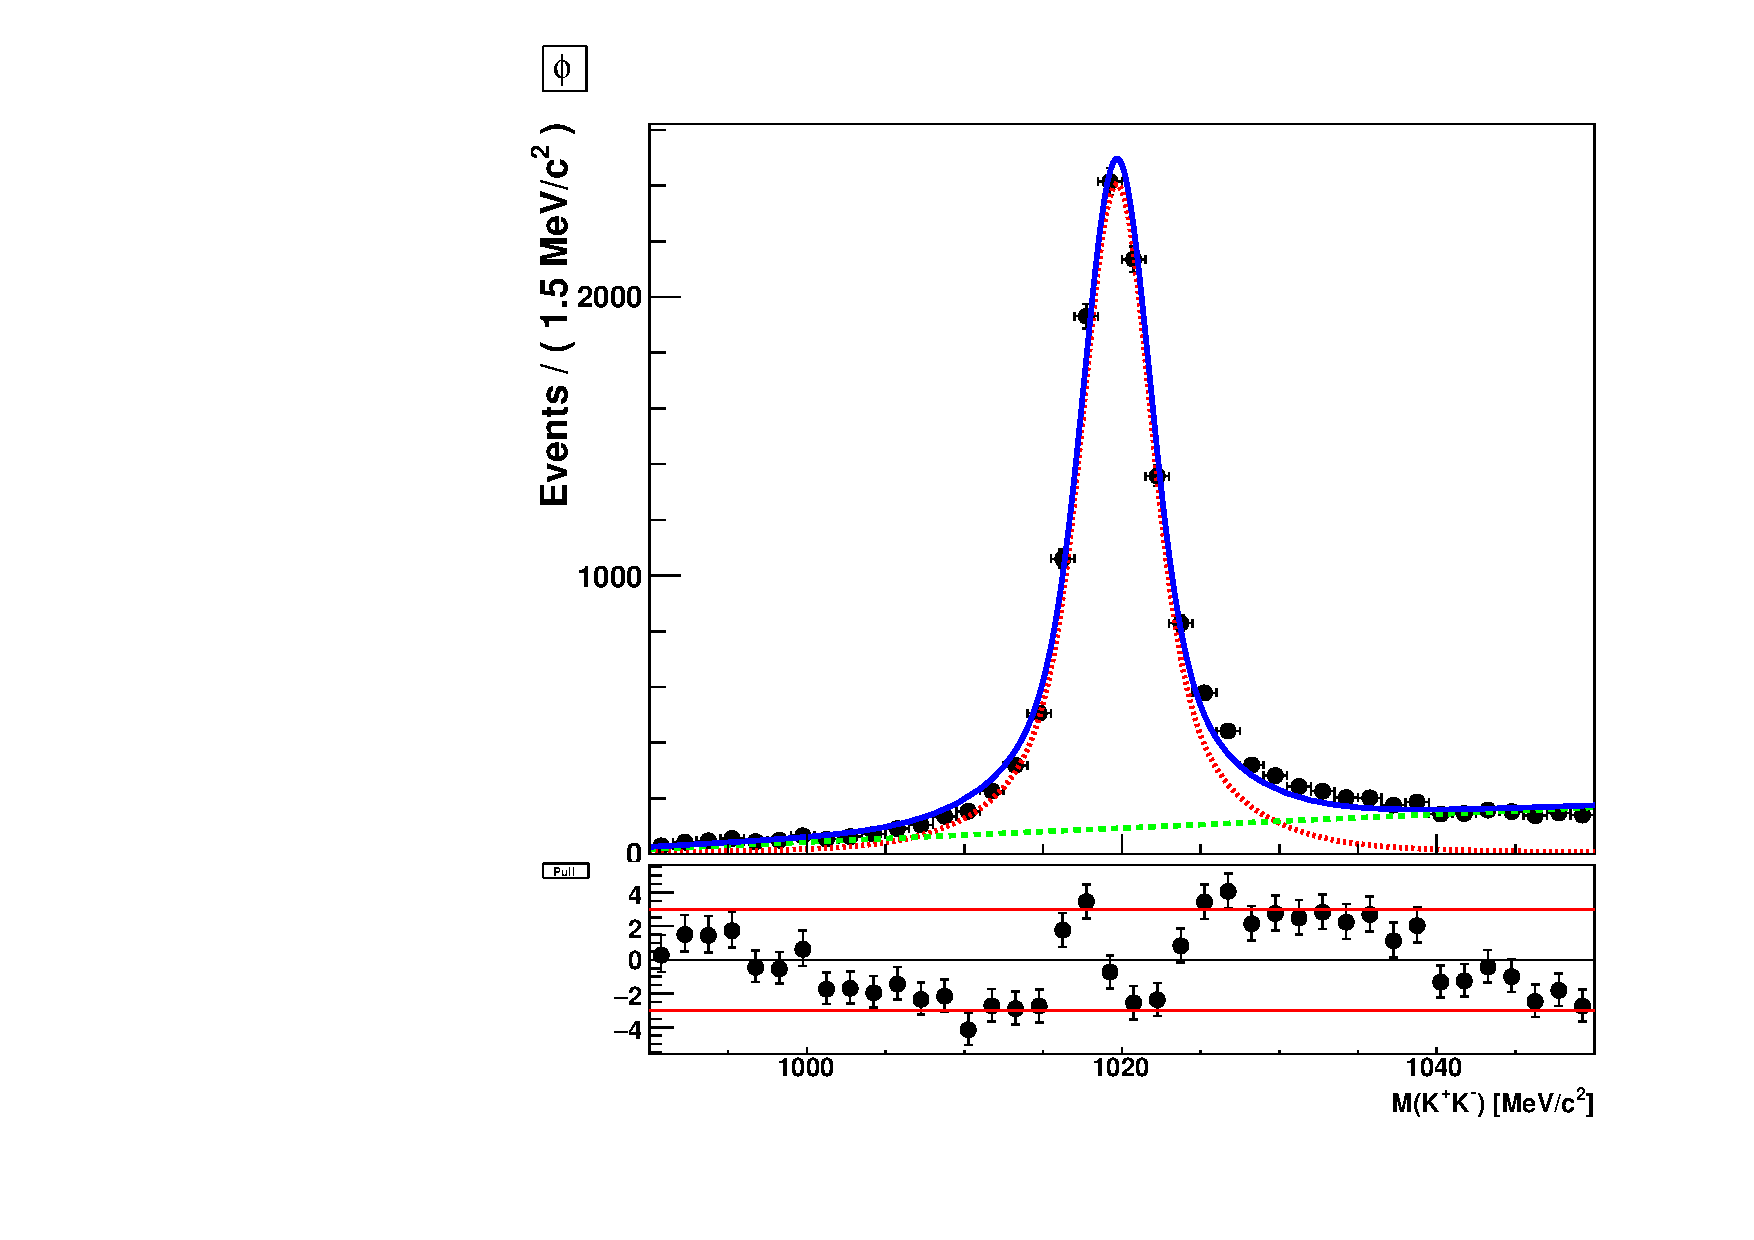
\includegraphics[width=0.49\linewidth]{RDfull_BDT1_BDT2_sWeight/mdau2.pdf}\put(-115,-4){(b)}
  \end{center}
  \caption{
   The invariant mass distributions of the (a) $\jpsi\to\epem$ and (b) $\phi\to\Kp\Km$ systems for the selected data sample of $\Bs\to\jpsi\phi$ candidates. The solid blue line shows the total fit, the signal and combinatorial background components are given by dotted red line and dashed green line, respectively.
}
  \label{fig:JpsiPhimass}
\end{figure}
\begin{table}[htb]
  \caption{
    The signal and the background yields from fits to the $\jpsi$ and $\phi$ mass distributions, separately in 2011 and 2012.
}
\small{
\begin{center} \begin{tabular}{|c|c|c|}
    \hline
   Year & 2011 & 2012  \\
    \hline
  $\jpsi$ bkg & 771$\pm$57 & 1 525$\pm$88\\
  $\jpsi$ signal & 3 833$\pm$79 & 9 551$\pm$126\\
  \hline
  \hline
  $\phi$ bkg & 990$\pm$48 & 2 632$\pm$69\\
  $\phi$ signal & 3 613$\pm$70 & 8 444$\pm$103\\
  \hline
    \end{tabular}\end{center}
  }
\label{tab:JpsiPhiTable}
\end{table}

For the $\Bs$ mass fit a signal model composed of a two Crystal Ball functions with a common mean is performed. The background model consists of an exponential fucntion for the combinatorial component and a Gaussian function for the partially reconstructed events (Fig.~\ref{fig:Bsmass}a). The partially reconstructed background (Bkg2) consists mainly of excited charmonium resonances and will be described in Sec.~\ref{subsubsec:PartRecBkg}. The fitted parameter values for the two 2011 and 2012 data samples are given in Table~\ref{tab:BsTable}, along with the signal and two background yields. 

\begin{figure}[htb!]
  \begin{center}
  \begin{minipage}[t]{0.48\linewidth}
  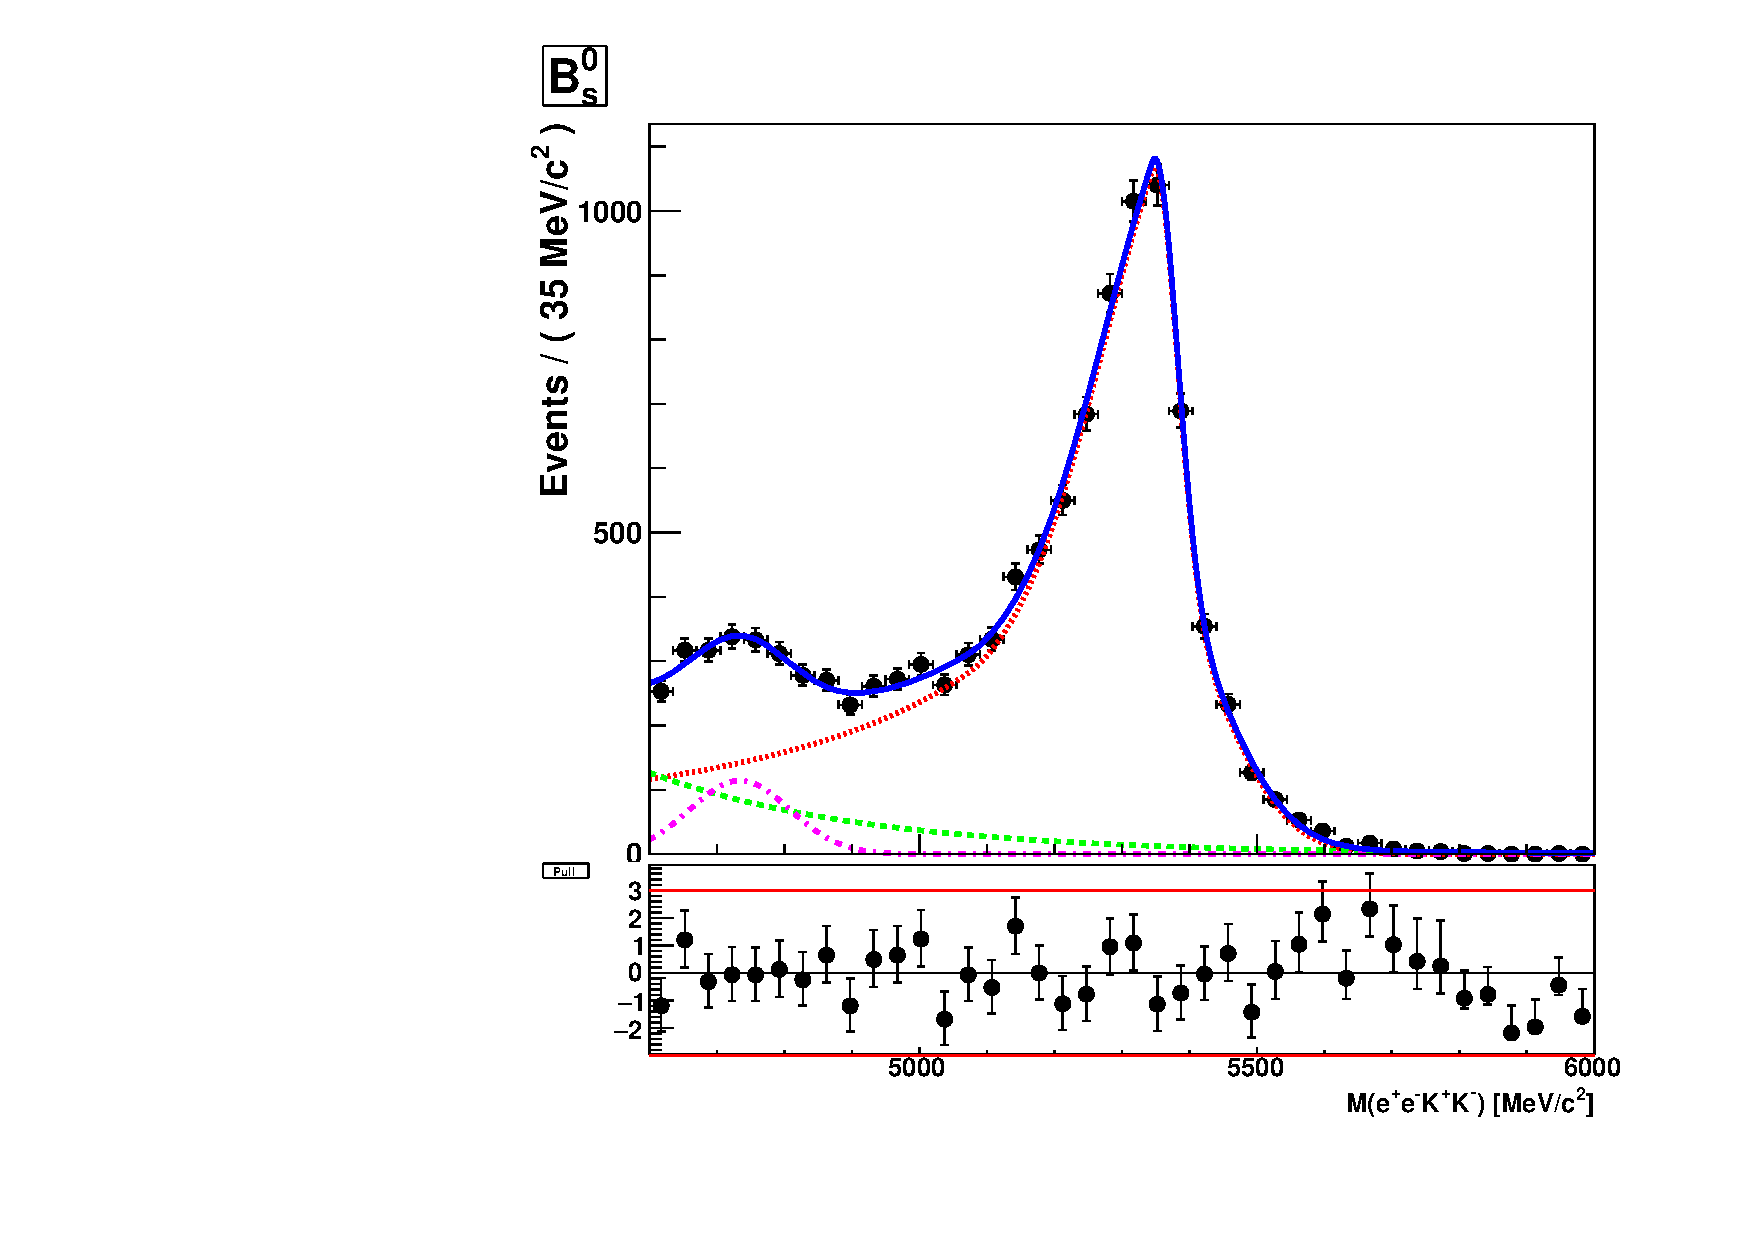
\includegraphics[width=1.1\linewidth]{RDfull_BDT1_BDT2_sWeight/mass_std.pdf}
  \end{minipage}
  \hfill
  \begin{minipage}[t]{0.48\linewidth}
  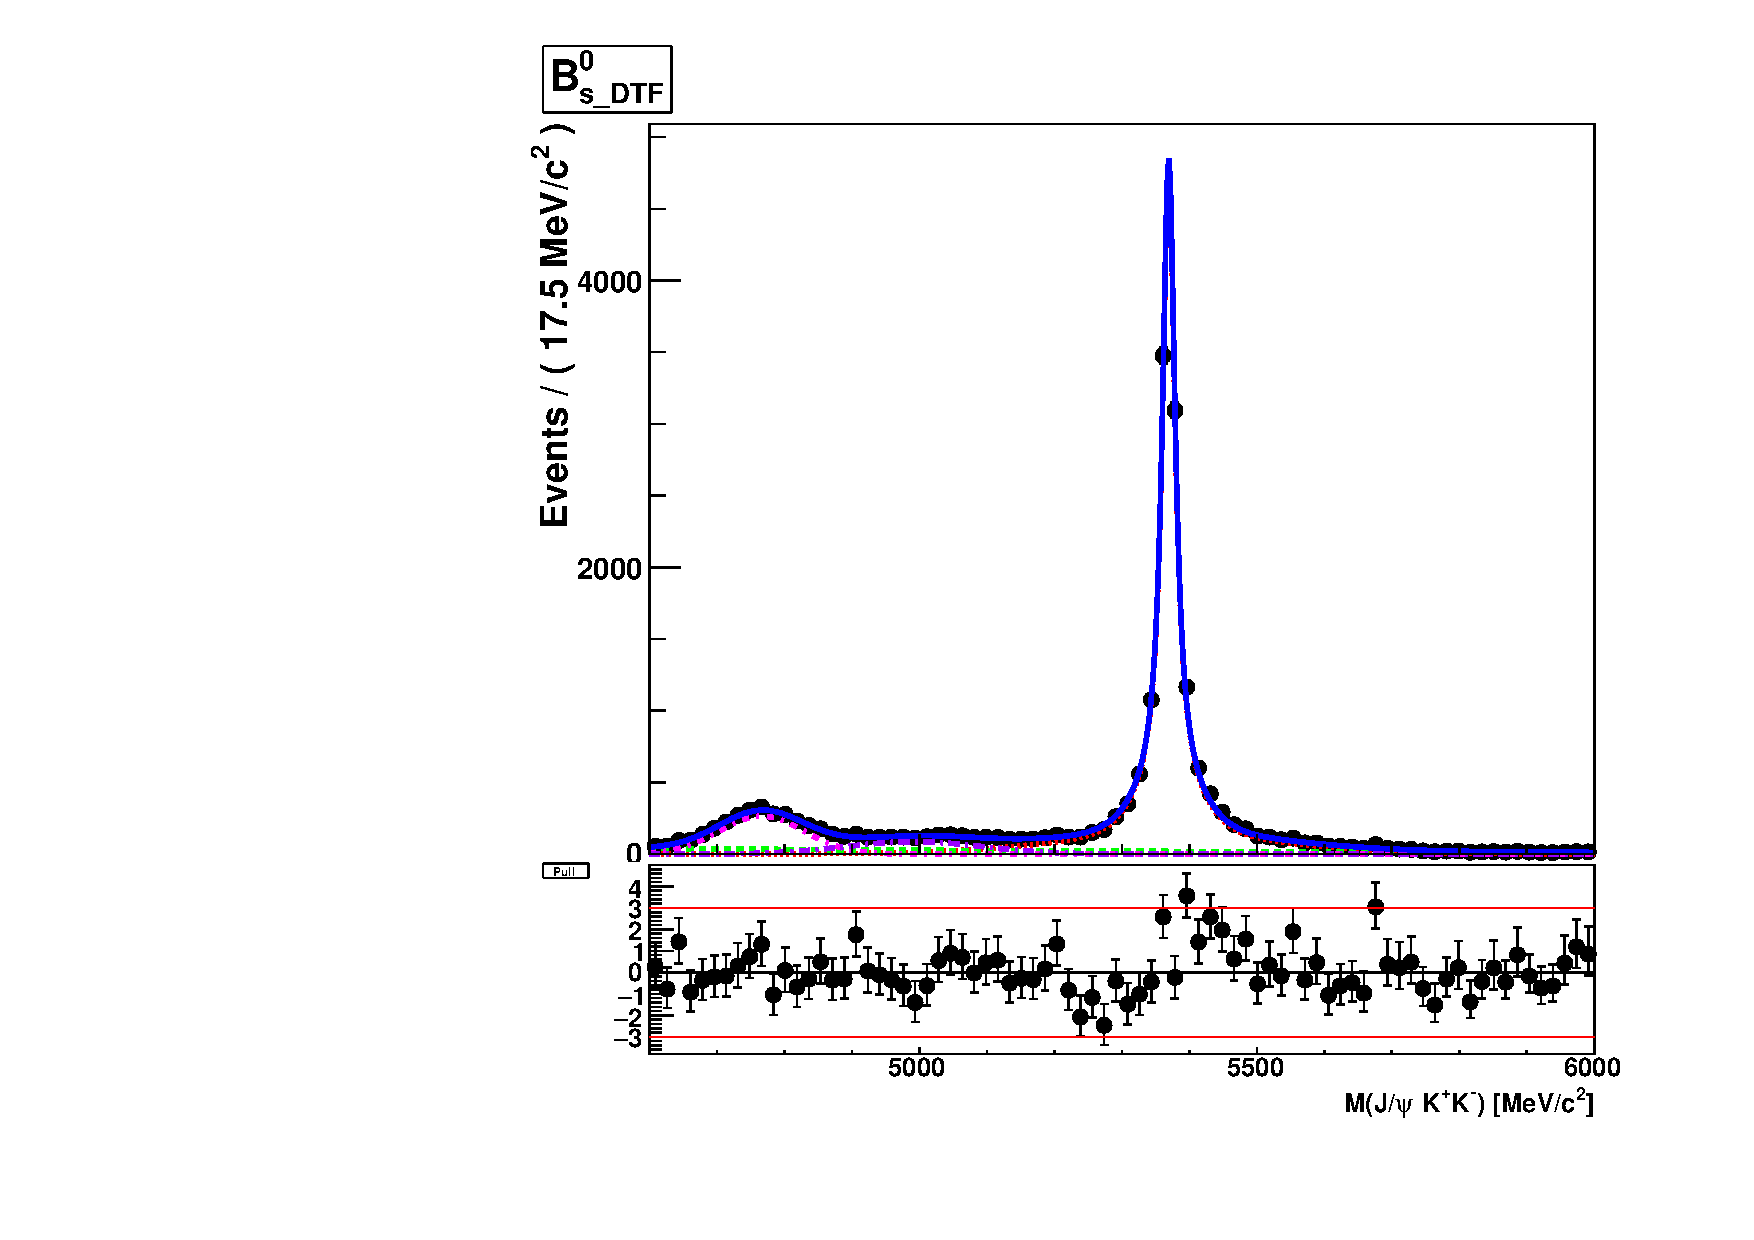
\includegraphics[width=1.1\linewidth]{RDfull_BDT1_BDT2_sWeight/mass.pdf}
  \end{minipage}
  \begin{minipage}[t]{0.48\linewidth}
  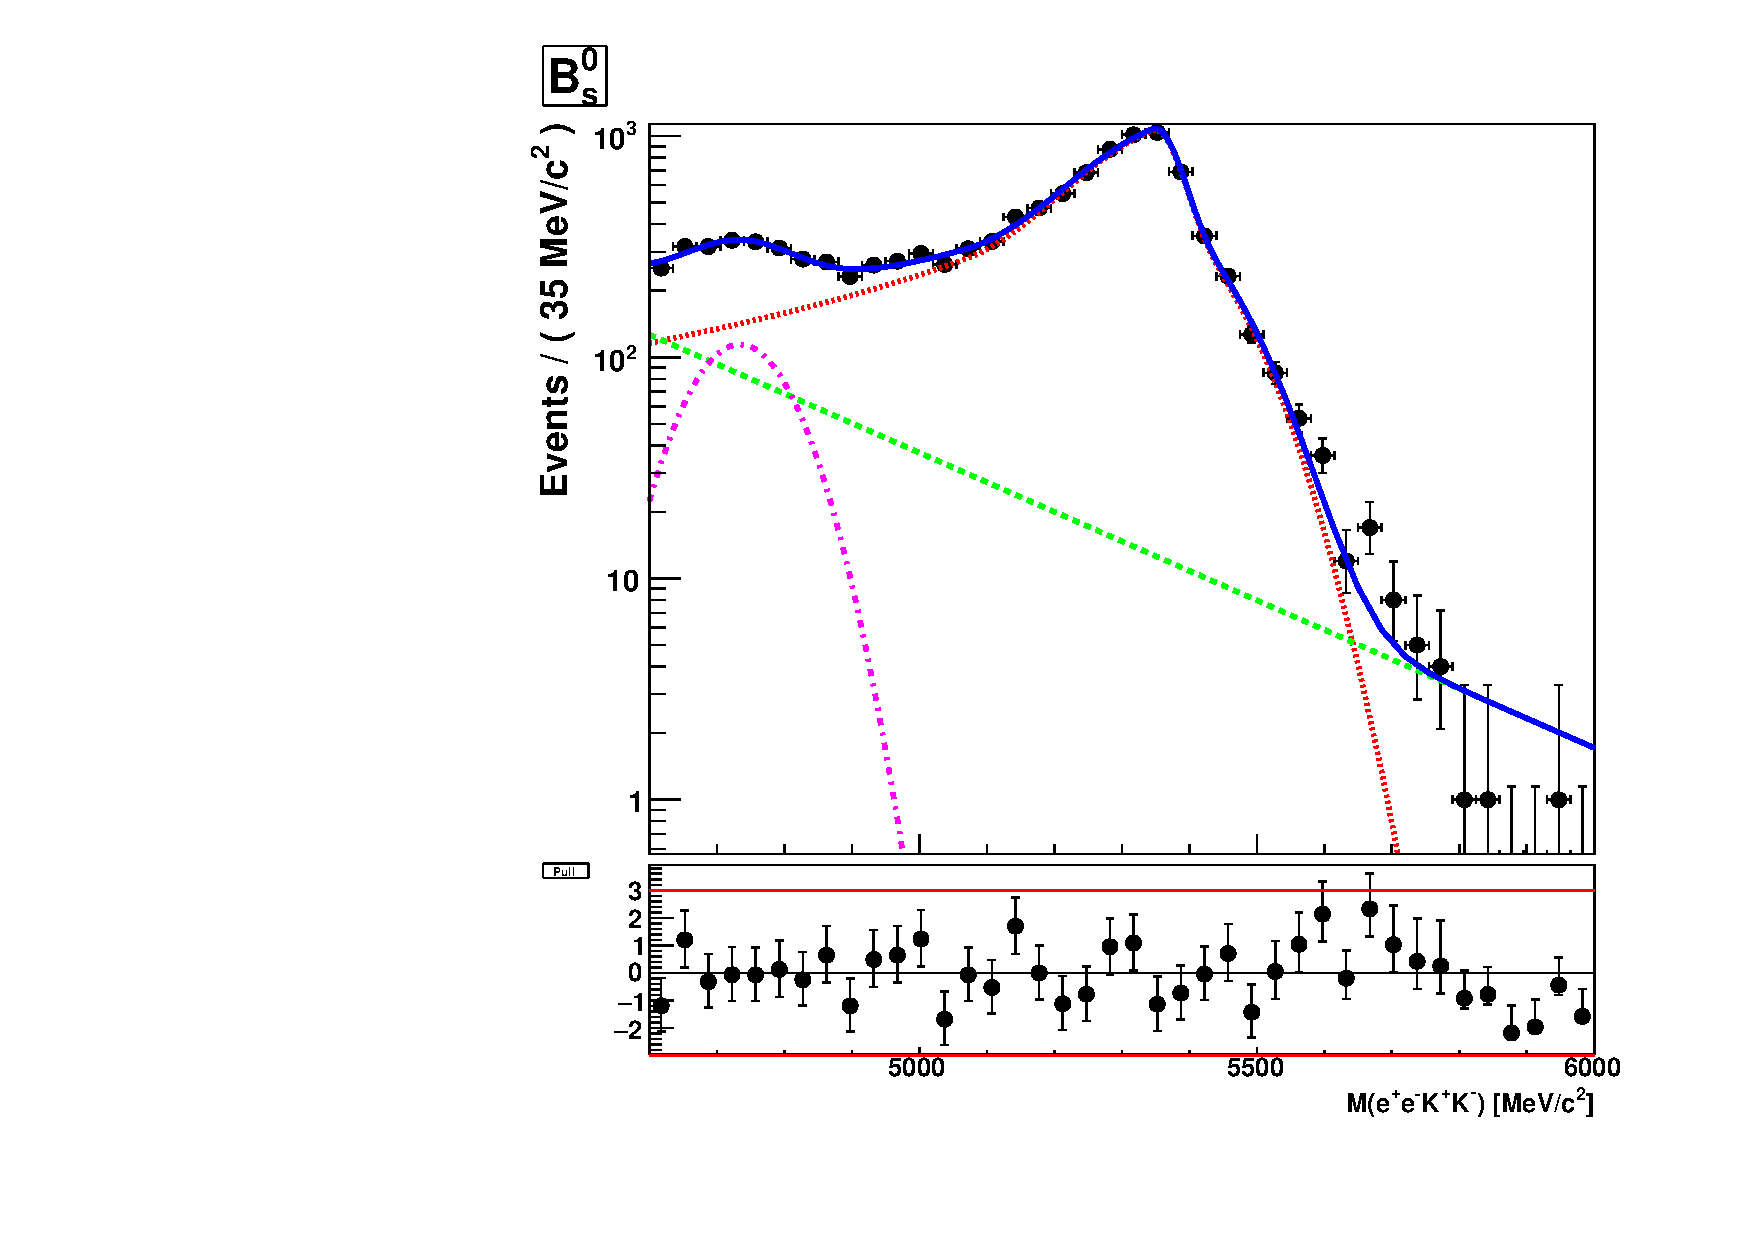
\includegraphics[width=1.1\linewidth]{RDfull_BDT1_BDT2_sWeight/mass_std_log.pdf}\put(-115,-4){(a)}
  \end{minipage}
  \hfill
  \begin{minipage}[t]{0.48\linewidth}
  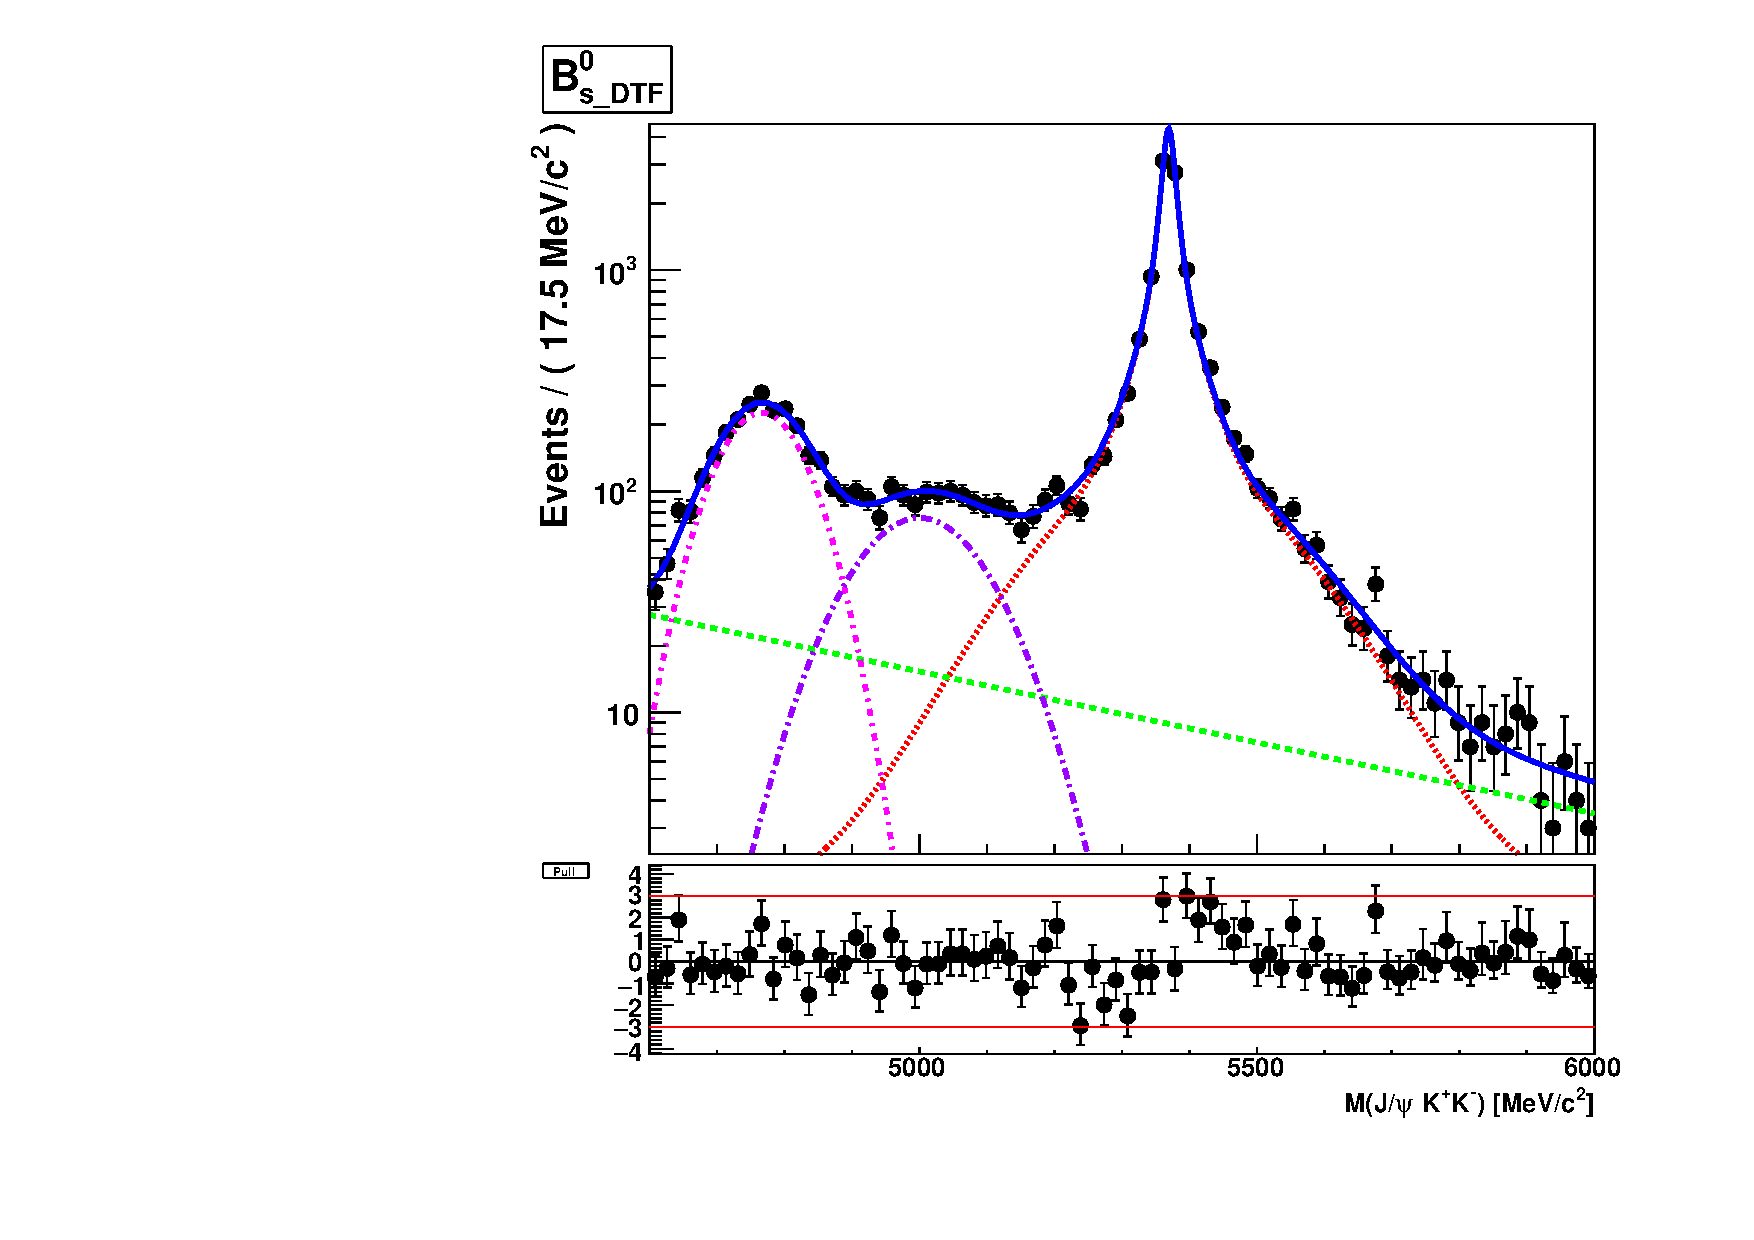
\includegraphics[width=1.1\linewidth]{RDfull_BDT1_BDT2_sWeight/mass_log.pdf}\put(-115,-4){(b)}
  \end{minipage}
  \end{center}
  \caption{
   The invariant mass distributions of the (a) $\Bs$ and (b) $\Bs$ using DTF in the selected data sample of $\Bs\to\jpsi\phi$ candidates. The solid blue line shows the total fit, the signal and combinatorial background components are given by dashed red line and dotted green line, respectively. The partially reconstructed background contributions are given by dash-dotted pink and violet lines. The top and bottom plots are linear and logarithmic scale, respectively.
}
  \label{fig:Bsmass}
\end{figure}

The $\Bs$ mass distribution with the mass of $\epem$ system constrained to the PDG mass of $\jpsi$~\cite{PDG2014}, obtained using Decay Tree Fitter (DTF), is shown in Fig.~\ref{fig:Bsmass}b. The mass model is a sum of double Gaussian and Breit-Wigner functions with a common mean for the signal candidates. The model describing combinatorial background is an exponential, two Gaussian functions are used to describe the partially reconstructed background (Sec.~\ref{subsubsec:PartRecBkg}). The fitted parameter values for the two 2011 and 2012 data samples are shown in Table~\ref{tab:BsDTFTable}, along with the signal and three  background yields. The number of signal events is 11 645$\pm$114 for the full 2011 and 2012 data sample, which corresponds to 12$\%$ of the signal events from the $\mumu$ decay mode of $\Bs\to\jpsi\phi$. 

The mass fit results for the $\Bs$ without and with DTF are in agreement to each other. The $\Bs$ mass distributions in a logarithmic scale are shown in Fig.~\ref{fig:Bsmass}.

\begin{table}[hb]
  \caption{
    The results of the fit to the $\Bs$ mass distribution, separately for 2011 and 2012 data samples. The signal shape is modeled by a sum of the two Crystal Ball functions with a common mean. The partially reconstructed background is modeled as a Gaussian function. The combinatorial background shape is an exponential.
}
\small{
\begin{center} \begin{tabular}{|c|c|c|}
   \hline
      Parameter & 2011 & 2012  \\
    \hline
   $\alpha^{CB}_{1}$ & 1.90$\pm$0.510 & 2.60$\pm$1.20\\
   $\alpha^{CB}_{2}$ & 0.10$\pm$0.062 & 0.15$\pm$0.02\\
   $\sigma_{1}$[$\mevcc$] & 100$\pm$3.1 & 100$\pm$0.45  \\
   $\sigma_{2}$[$\mevcc$] & 29$\pm$3.3 & 33$\pm$1.4  \\
   $\sigma_{Bkg2}$[$\mevcc$] & 68$\pm$26 & 74$\pm$8.3  \\
   $\mu$[$\mevcc$] & 5 353$\pm$3.9 & 5 349$\pm$1.7 \\
   $\mu_{Bkg2}$[$\mevcc$] & 4 739$\pm$20 & 4 734$\pm$8.8  \\
   $f$ & 0.336$\pm$0.070 & 0.304$\pm$0.053  \\
   Bkg slope & -0.0034$\pm$0.0004 & -0.0031$\pm$0.00002 \\
   N$_{Bkg1}$ & 689$\pm$77 & 586$\pm$76  \\
   N$_{Bkg2}$ & 258$\pm$48 & 1 163$\pm$123 \\
   N$_{Sig}$ & 3 656$\pm$73 & 9 327$\pm$119 \\
  \hline
    \end{tabular}\end{center}
  }
\label{tab:BsTable}
\end{table}
\begin{table}[htb]
  \caption{
    The results of the fit to the $\Bs$ mass distribution with DTF, separately for 2011 and 2012 data samples. The signal shape is a sum of double Gaussian and Breit-Wigner functions with a common mean. The two partially reconstructed backgrounds are modeled by two Gaussians. The combinatorial background shape is an exponential function.
}
\small{
\begin{center} \begin{tabular}{|c|c|c|}
    \hline
   Parameter & 2011 & 2012  \\
    \hline
  $\sigma_{1}$[MeV/c$^{2}$] & 147$\pm$23 &158$\pm$12\\
  $\sigma_{2}$[MeV/c$^{2}$] & 8.1$\pm$0.92 &45$\pm$6.3\\
  $\sigma_{3}$[MeV/c$^{2}$] & 50$\pm$11 &23$\pm$1.1\\
  $\sigma_{bkg2}$[MeV/c$^{2}$] & 60$\pm$6.3 &65$\pm$4.4\\
  $\sigma_{bkg3}$[MeV/c$^{2}$] & 109$\pm$20 &90$\pm$9.2\\
  $f_{1}$ & 0.11$\pm$0.035 &0.17$\pm$0.017\\
  $f_{2}$ & 0.24$\pm$0.065 &0.12$\pm$0.026\\
  $\mu$[MeV/c$^{2}$] & 5370$\pm$0.36 &5370$\pm$0.23\\
  $\mu_{bkg2}$[MeV/c$^{2}$] & 4757$\pm$5.2 & 4770$\pm$3.4\\
  $\mu_{bkg3}$[MeV/c$^{2}$] & 4978$\pm$25 & 5006$\pm$9.8\\
  bkg slope & -0.0015$\pm$0.0005 & -0.0018$\pm$0.0004\\
  N$_{bkg}$ & 340$\pm$57 & 544$\pm$78\\
  N$_{bkg2}$ & 587$\pm$33 & 1 470$\pm$52\\
  N$_{bkg3}$ & 307$\pm$31 & 727$\pm$41\\
  N$_{sig}$ & 3 369$\pm$62 & 8 336$\pm$96\\
  \hline
    \end{tabular}\end{center}
  }
\label{tab:BsDTFTable}
\end{table}

The fit performed to the reconstructed $\jpsi(\epem)\phi$ mass distribution with DTF (Fig.~\ref{fig:Bsmass}b) is used to generate the event weights (sWeights) using the sPlot technique~\cite{Pivk:2004ty}. The weights are used in the time dependent angular analysis. The fits to the $\jpsi$, $\phi$ and $\Bs$ mass distributions are not subsequently used in the analysis and they simply help to illustrate the data sample.


\subsection{Background components}
\subsubsection{Combinatorial background}

The random combinatorial background arises when not all of the four tracks originate from the $\Bs$ meson. This is modeled by an exponential function, the slope of which is left floating in the fit cases. 

\subsubsection{Partially reconstructed background}\label{subsubsec:PartRecBkg}

The partially reconstructed background arises from the true $\Bs$ decays but with one or more tracks missing in the reconstruction. In the case of $\Bs\to\jpsi(\epem)\phi$, there are two sources for these partially reconstructed events: those are from the hadronic part, such as events with $\phi(1020)$ resonance, called partially reconstructed hadronic background in the following, and those are from the $\jpsi$ part, called partially reconstructed $\jpsi$ background in the following, such as events from $\psi(2S)$ and $\chi_{c1}(1P)$ decays. In order to study the background, a dedicated inclusive $\Bs\to\jpsi(\epem)X$ MC sample is used. The sample consists of 8 million events and is required to pass all selection cuts, as well as a veto on true $\Bs\to\jpsi(\epem)\phi$ events. The surviving events are split into four categories:
\begin{itemize}
 \item both the $\jpsi$ and the $\phi$ mesons are decay products of the $\Bs$ meson;
 \item the $\jpsi$ meson originates from excited charmonium resonances;
 \item the $\phi$ meson is a product of one of the hadronic resonances;
 \item neither $\jpsi$ nor $\phi$ are decay products of the $\Bs$ meson.
\end{itemize}
The $\Bs$ mass distribution with the reconstructed $\jpsi$ mass and constraint $\jpsi$ mass for all categories are shown in Fig.~\ref{fig:PartReconBkg} and~\ref{fig:PartReconBkg_Jpsi}. Most of the events are from the $\jpsi$ part (black points in Fig.~\ref{fig:PartReconBkg}) where 46.9$\%$ is from $\psi(2S)$ decaying into $\jpsi$ and 35.4$\%$ originates from $\chi_{c1}(1P)$ decays. The remaining part of the events comes from $\chi_{c0}(1P)$ (0.4$\%$), $\chi_{c2}(1P)$ (1.7$\%$) and $h_{c}(1P)$ (0.6$\%$) decays as shown in Fig.~\ref{fig:PartReconBkg_Jpsi}. The 15$\%$ of the events account for the "none" type (default code 0 for a particle~\cite{Sjostrand:2006za}) that mean pure phase space decays, according to the given branching ratios. Only 4$\%$ of partially reconstructed background is due to the hadronic part (blue points in Fig.~\ref{fig:PartReconBkg}) which is $\eta^{'}$, $B^{0\ast}_{s}$ and $b\bar{b}$ decays.  

The $\Bs\to\jpsi(\epem)X$ simulated sample is only used to distinguish the different type of partially reconstructed background in $\Bs$ mass distributions in the data sample. The mass fit is not applied to partially reconstructed background in the simulated sample.

\begin{figure}[htb]
  \begin{center}
    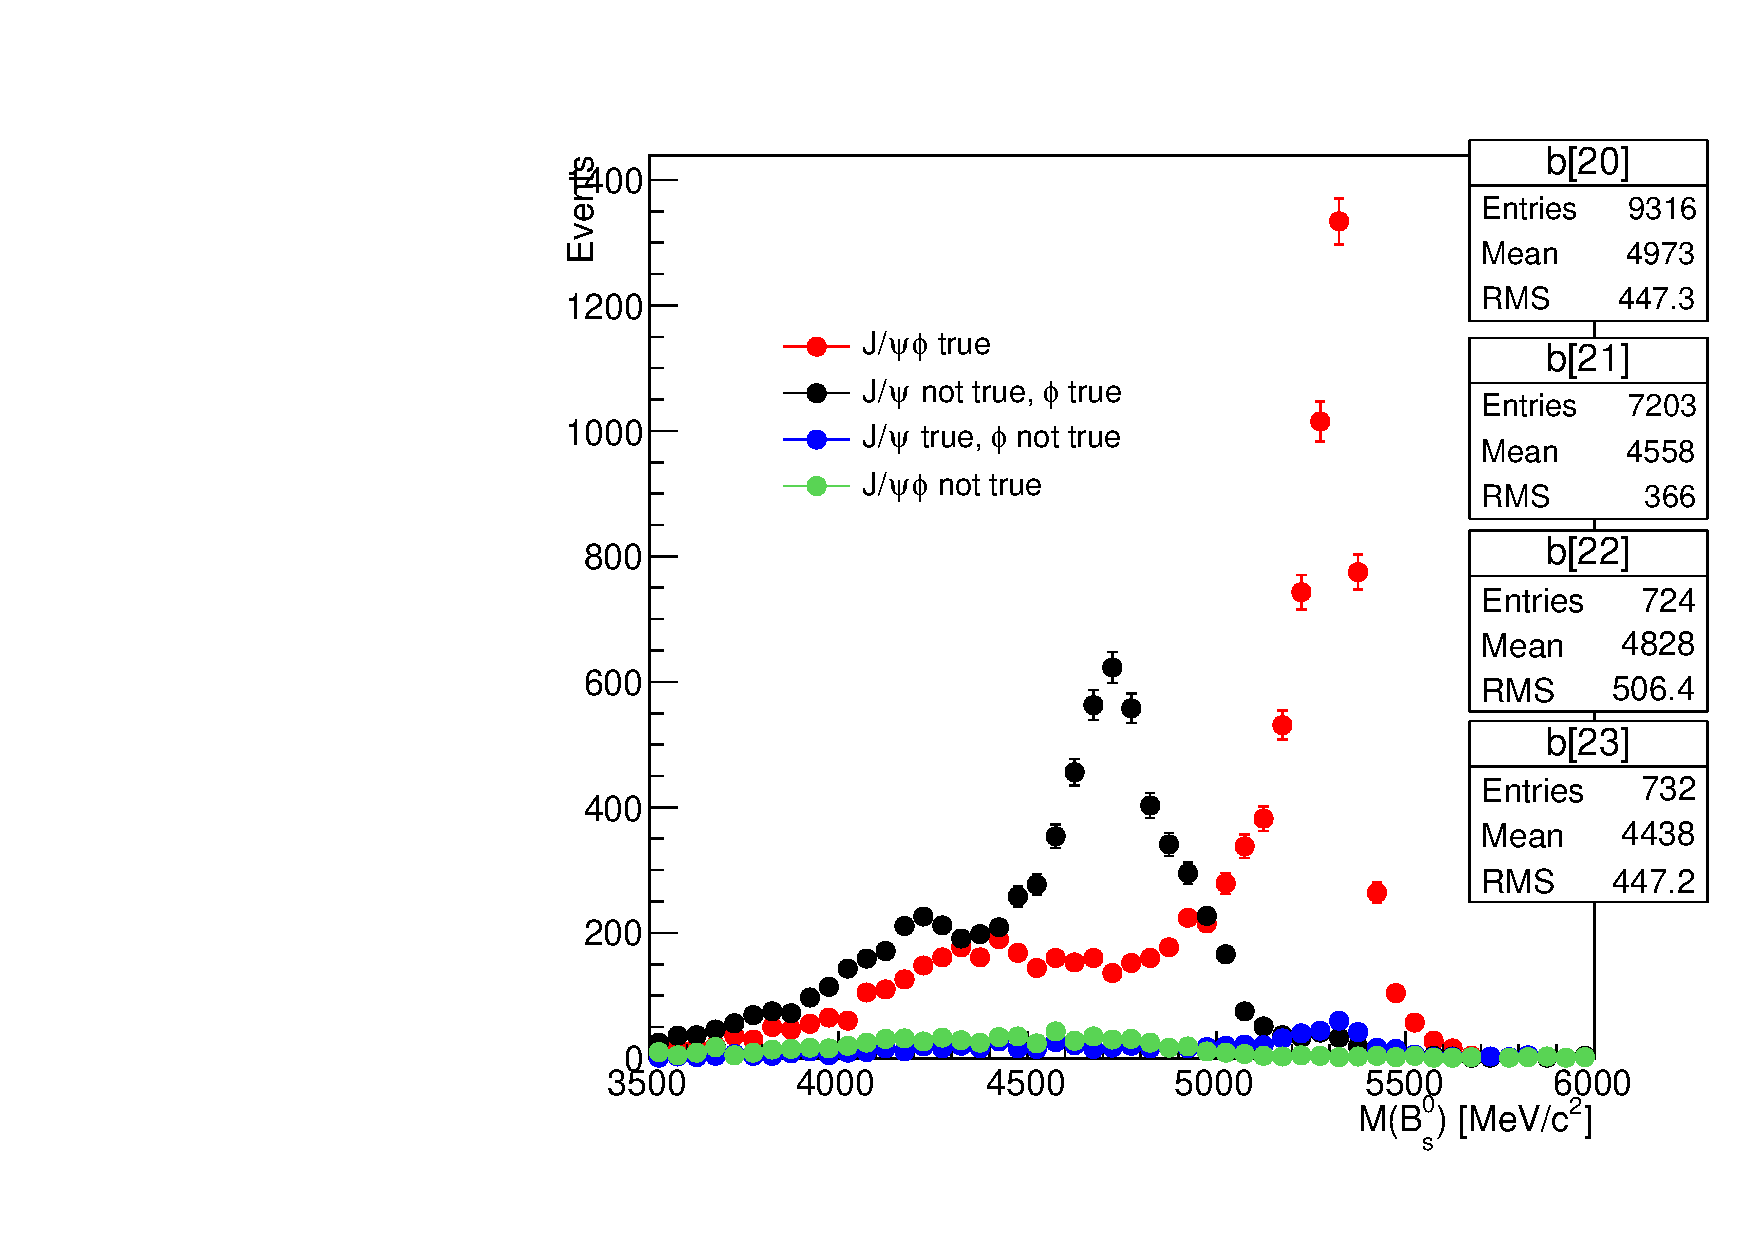
\includegraphics[width=0.52\linewidth]{Bkg2_BsDTF/Bs_M_Bs2JpsieeX_divideBkg_fullrange_newcuts.pdf}\put(-115,-4){(a)}
    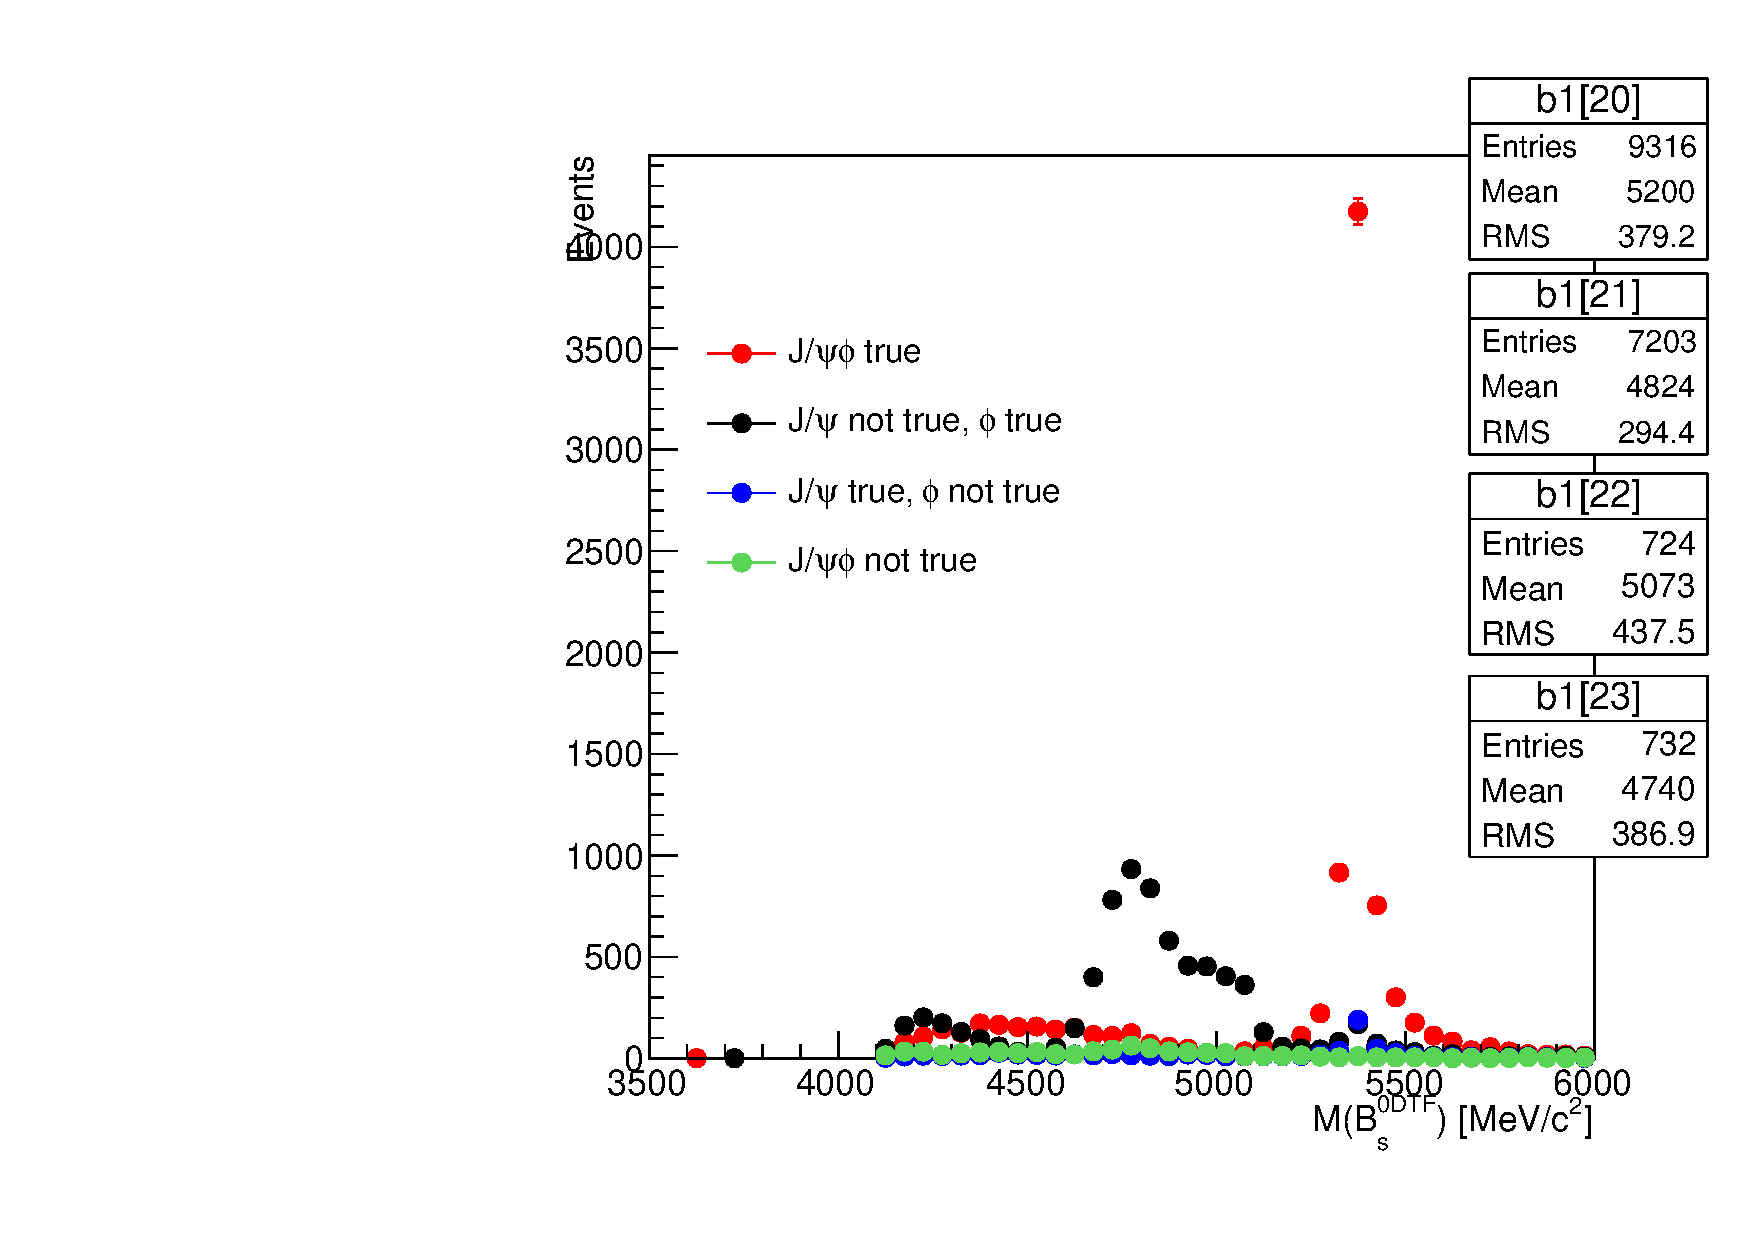
\includegraphics[width=0.52\linewidth]{Bkg2_BsDTF/BsDTF_M_Bs2JpsieeX_divideBkg_fullrange_newcuts.pdf}\put(-115,-4){(b)}
  \end{center}
  \caption{
   The background from partially reconstructed events due to missing particles from the $\jpsi$ and/or hadronic part: (a) $\Bs$ mass distribution, (b) $\Bs$ mass distribution using DTF.
}
  \label{fig:PartReconBkg}
\end{figure}
\begin{figure}[htb]
  \begin{center}
    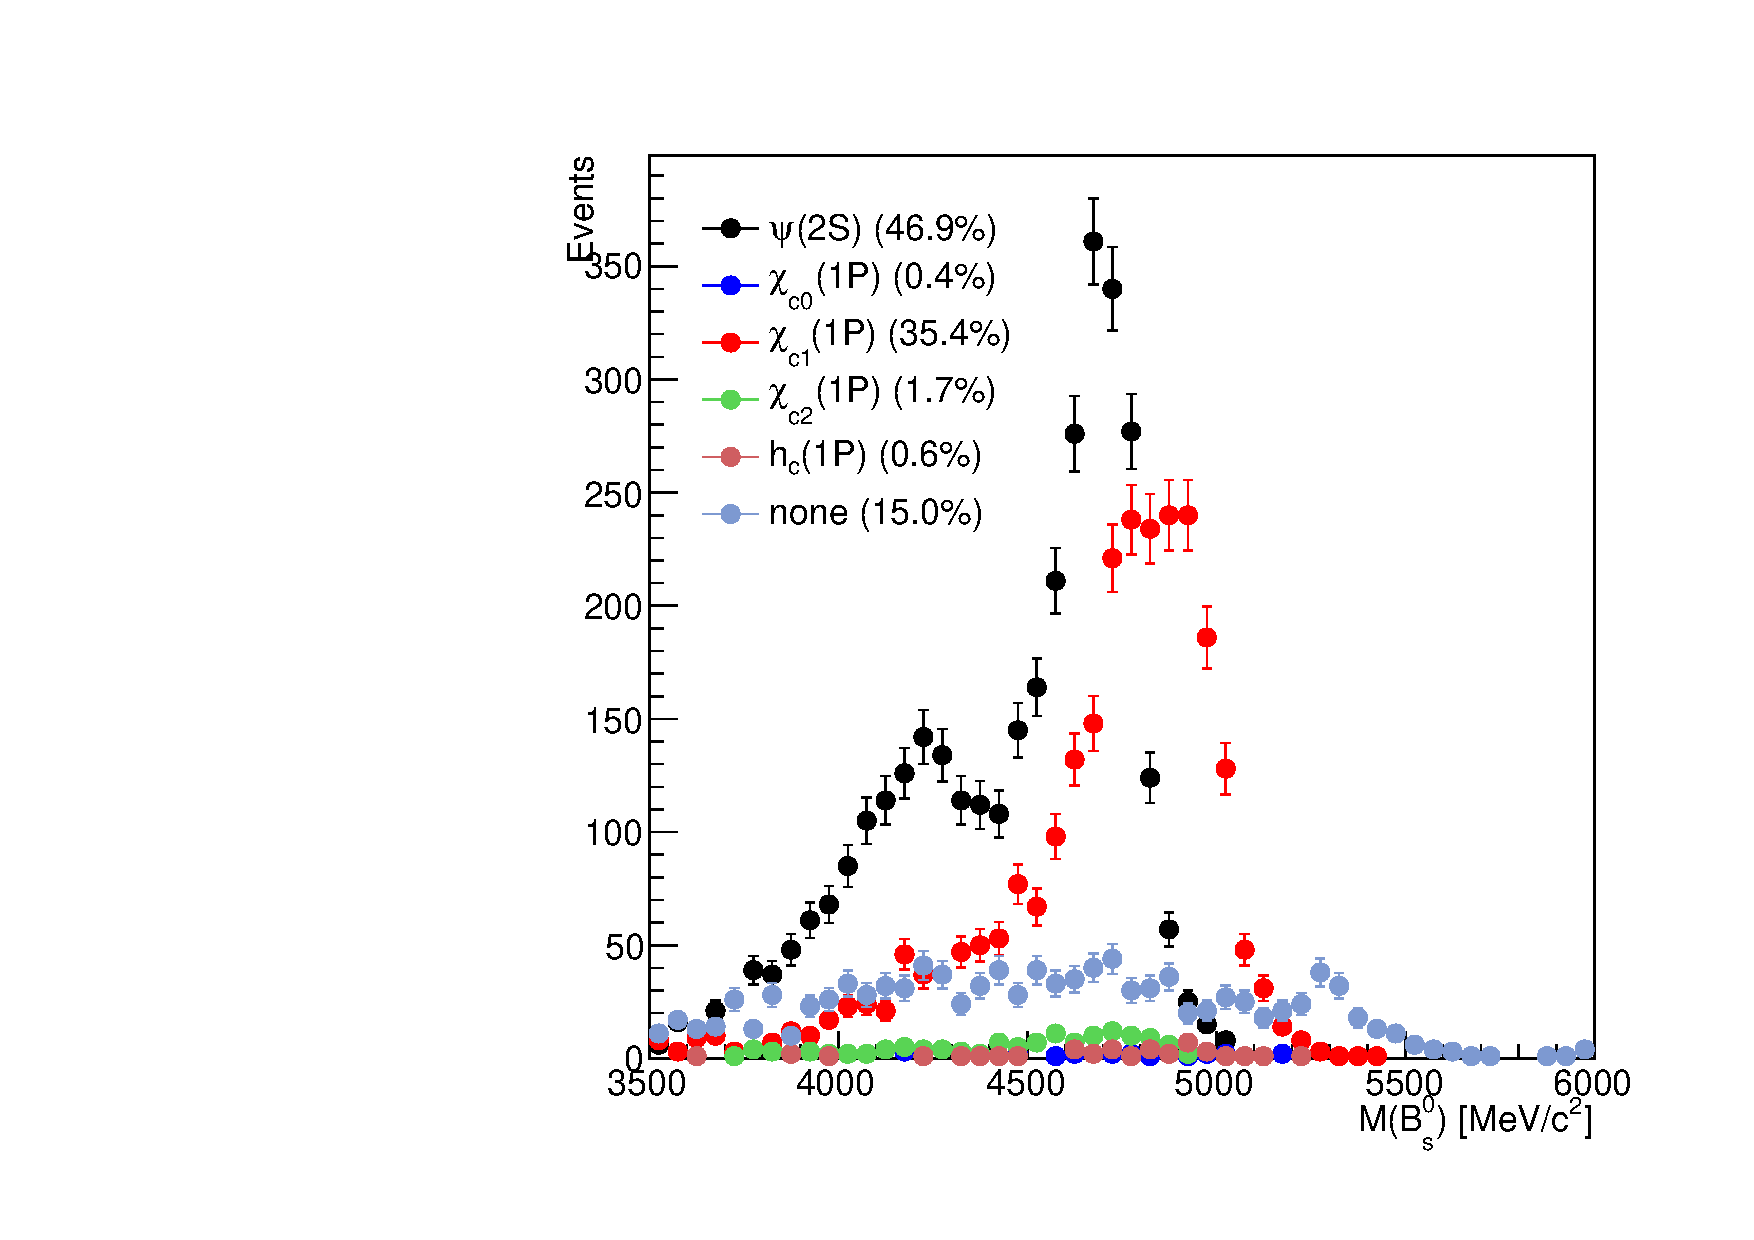
\includegraphics[width=0.52\linewidth]{Bkg2_BsDTF/Bs_M_Bs2JpsieeX_JpsiBkg_fullrange_newcuts.pdf}\put(-115,-4){(a)}
    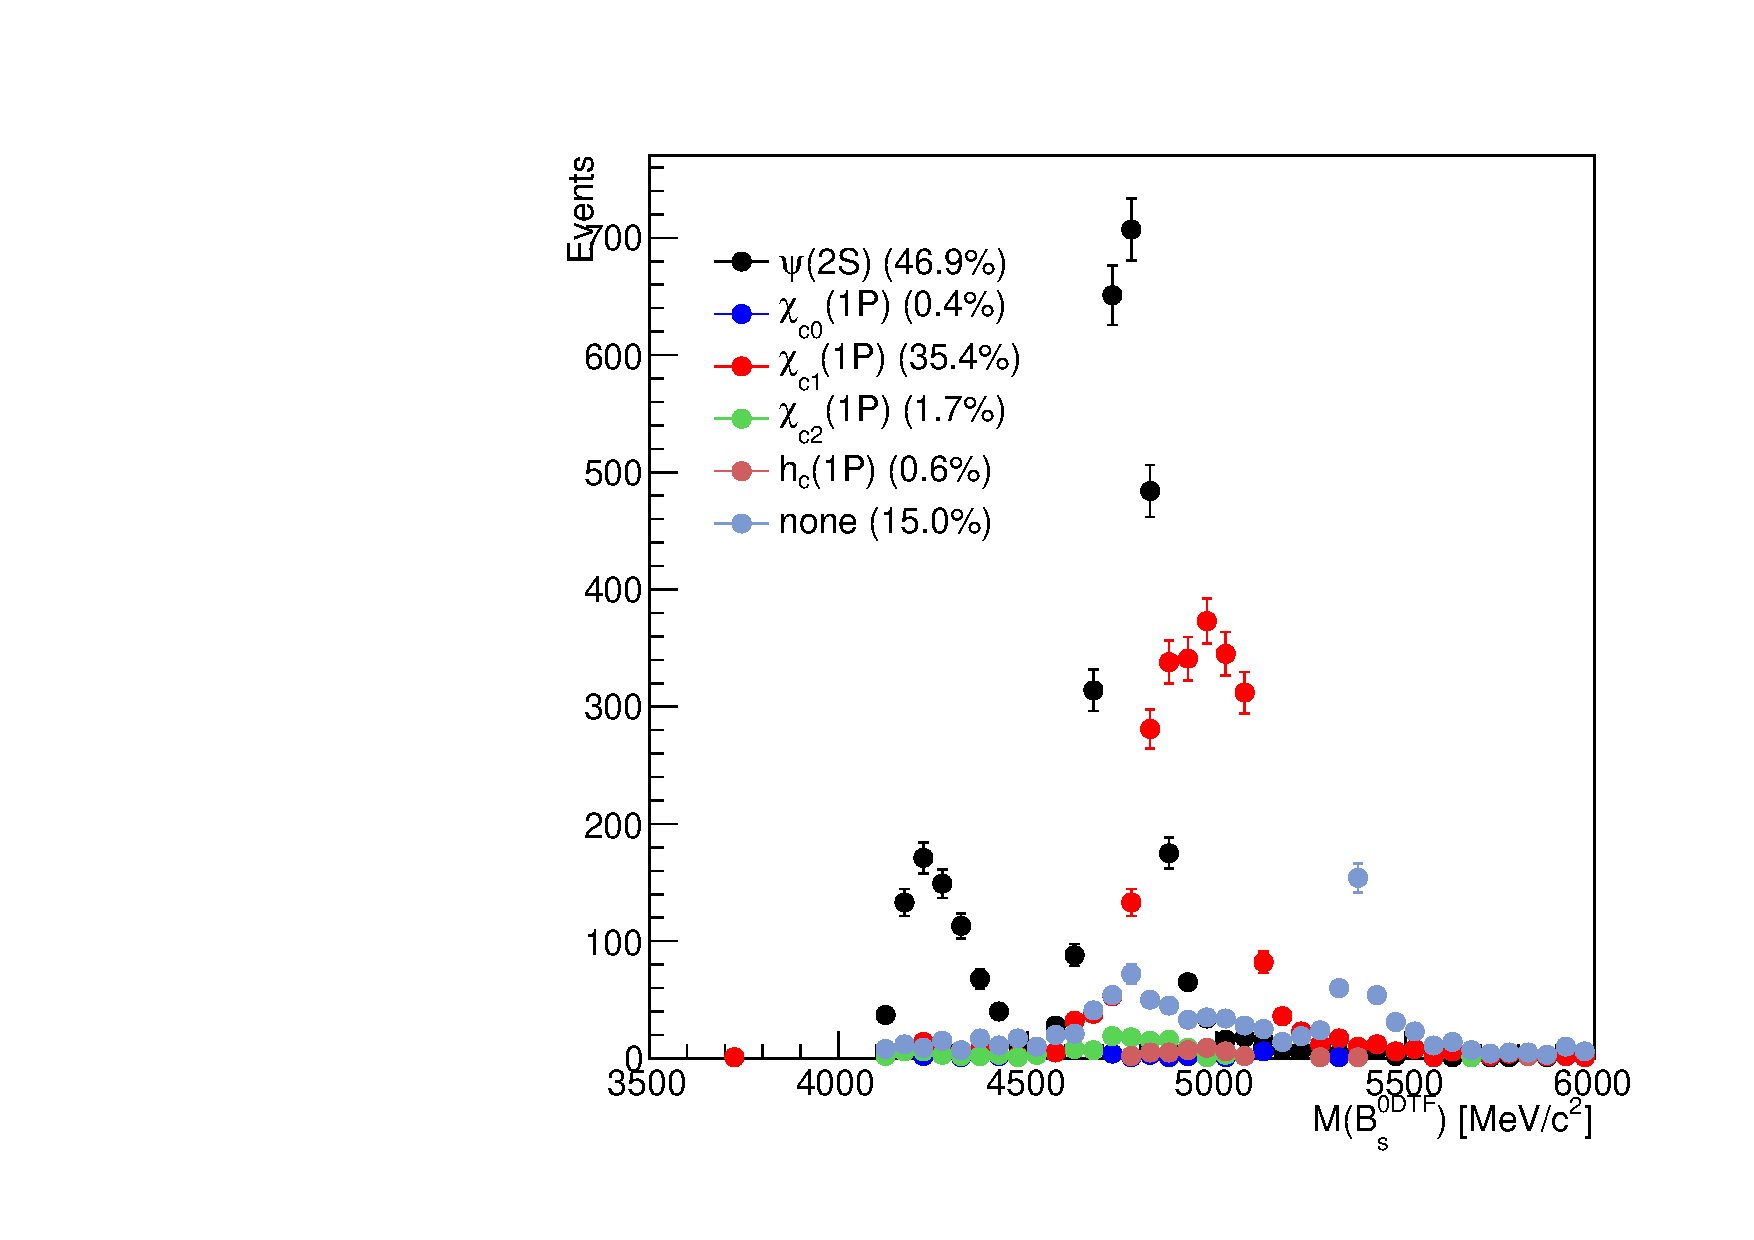
\includegraphics[width=0.52\linewidth]{Bkg2_BsDTF/BsDTF_M_Bs2JpsieeX_JpsiBkg_fullrange_newcuts.pdf}\put(-115,-4){(b)}
  \end{center}
  \caption{
   The $\jpsi$ partially reconstructed background from the excited charmonium resonances for (a) $\Bs$ mass distribution and (b) $\Bs$ mass distribution using DTF.
}
  \label{fig:PartReconBkg_Jpsi}
\end{figure}
\clearpage

\section{Decay time resolution}\label{sec:TimeRes}

The precision of the $\phis$ determination is dependent on the decay time resolution. As in the $\Bs\to\jpsi(\mumu)\Kp\Km$ analysis~\cite{Aaij:2014-039} it could be determined from a sample of prompt $\jpsi\to\epem$ events selected using the following decay time stripping and unbiased trigger lines:
\begin{itemize}
 \item Stripping line: {\tt StrippingBs2JpsieePhiLine}
 \item Unbiased triggers: {\tt L0ElectronDecision$\_$TOS} or {\tt L0HadronDecision$\_$TOS}
\end{itemize}
However, no $\jpsi\to\epem$ peak is observed in the data (Fig.~\ref{fig:JpsiPeak}a), even after testing different criteria to try and isolate the signal. The $\jpsi$ peak arises using a constraint $\Bs$ decay time $t>0.3$~$\ps$ (Fig.~\ref{fig:JpsiPeak}b). 
\begin{figure}[htb]
  \begin{center}
    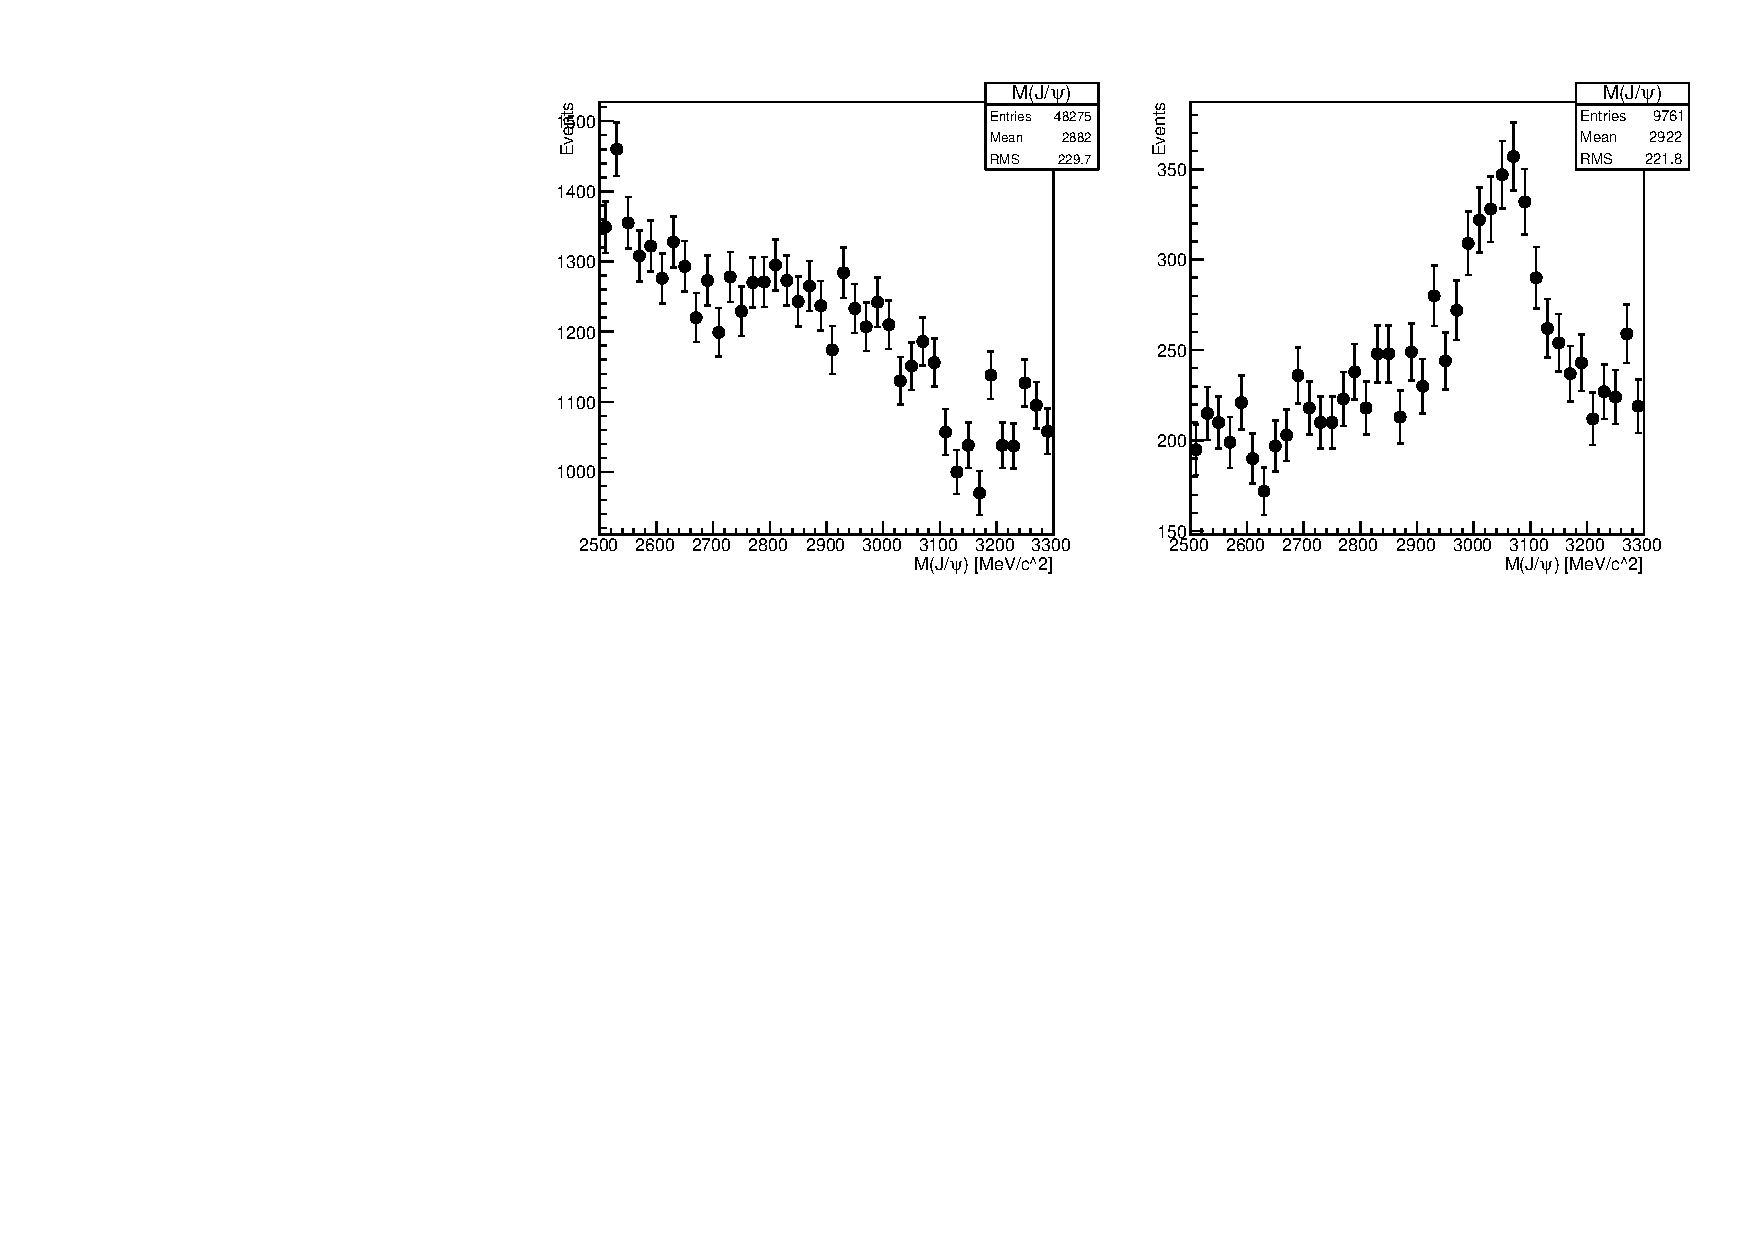
\includegraphics[width=0.9\linewidth]{TimeRes/Jpsi_M_allcuts_time03ps.pdf}\put(-315,-4){(a)} \put(-110,-4){(b)}
  \end{center}
  \caption{
   (a) The distribution of the $\jpsi\to\epem$ invariant mass for events selected using the {\tt Bs2JpsieePhiLine} stripping line with unbiased {\tt L0ElectronDecision$\_$TOS} and {\tt L0HadronDecision$\_$TOS} triggers. No clear sign of the $\jpsi\to\epem$ decays is visible. (b) The distribution of the $\jpsi\to\epem$ invariant mass for events selected using in addition the cut on the $\Bs$ decay time $t>0.3$~$\ps$. The peak from $\jpsi\to\epem$ decays is seen. 
}
  \label{fig:JpsiPeak}
\end{figure}

To solve this problem we compare the time resolution of the $\epem$ and $\mumu$ modes of the $\Bs\to\jpsi\phi$ decays, as the kinematics of these two modes are similar (see Appendix~\ref{sec:app:Comparison}). To do this the simulated signal events from the $\Bs\to\jpsi(\epem)\phi$ and $\Bs\to\jpsi(\mumu)\Kp\Km$ channels are used. A fit was performed to the difference between the true and reconstructed decay time for unbiased 2012 simulated events for both modes using the triple Gaussian resolution model. The $\Bs\to\jpsi(\epem)\phi$ unbiased events pass {\tt L0ElectronDecision$\_$TOS} or {\tt L0HadronDecision$\_$TOS} triggers. In case of the $\Bs\to\jpsi(\mumu)\Kp\Km$ decay, the unbiased sample includes events which passed {\tt Hlt2DiMuonDetachedJPsi$\_$TOS} and {\tt Hlt1DiMuonHighMass$\_$TOS} trigger lines. The parameters resulting from the fit are presented in Table~\ref{tab:TimeRes}. No sizable difference between the two modes is visible. Plots showing the fit to the difference in true and reconstructed decay time are depicted in Fig.~\ref{fig:TimeResMC12}. The time resolution of the $\Bs\to\jpsi(\epem)\phi$ decay is comparable with the time resolution of the $\Bs\to\jpsi(\mumu)\Kp\Km$ decay mode.
\begin{figure}[htb]
  \begin{center}
    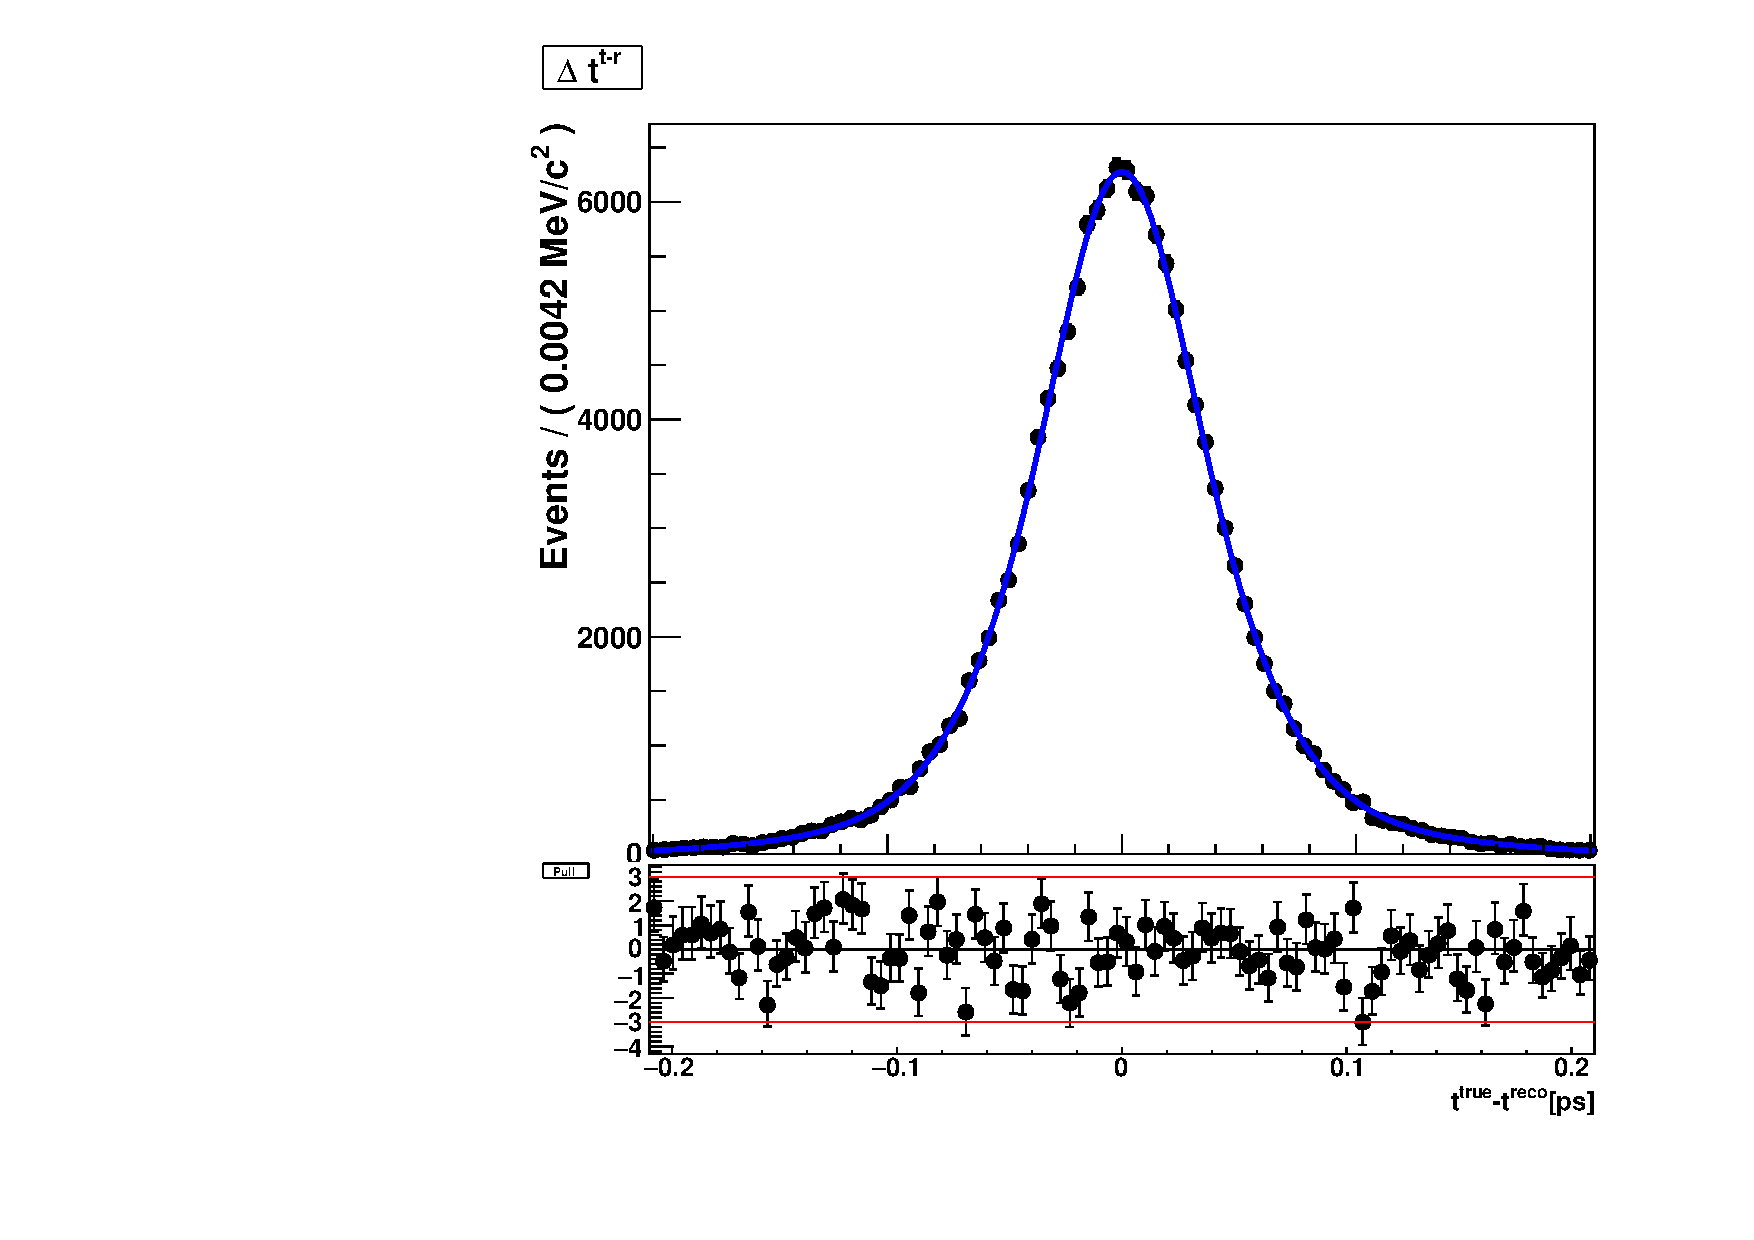
\includegraphics[width=0.49\linewidth]{TimeRes/time_diff_ps_MC12_unbias_pull.pdf}\put(-115,-4){(a)} 
    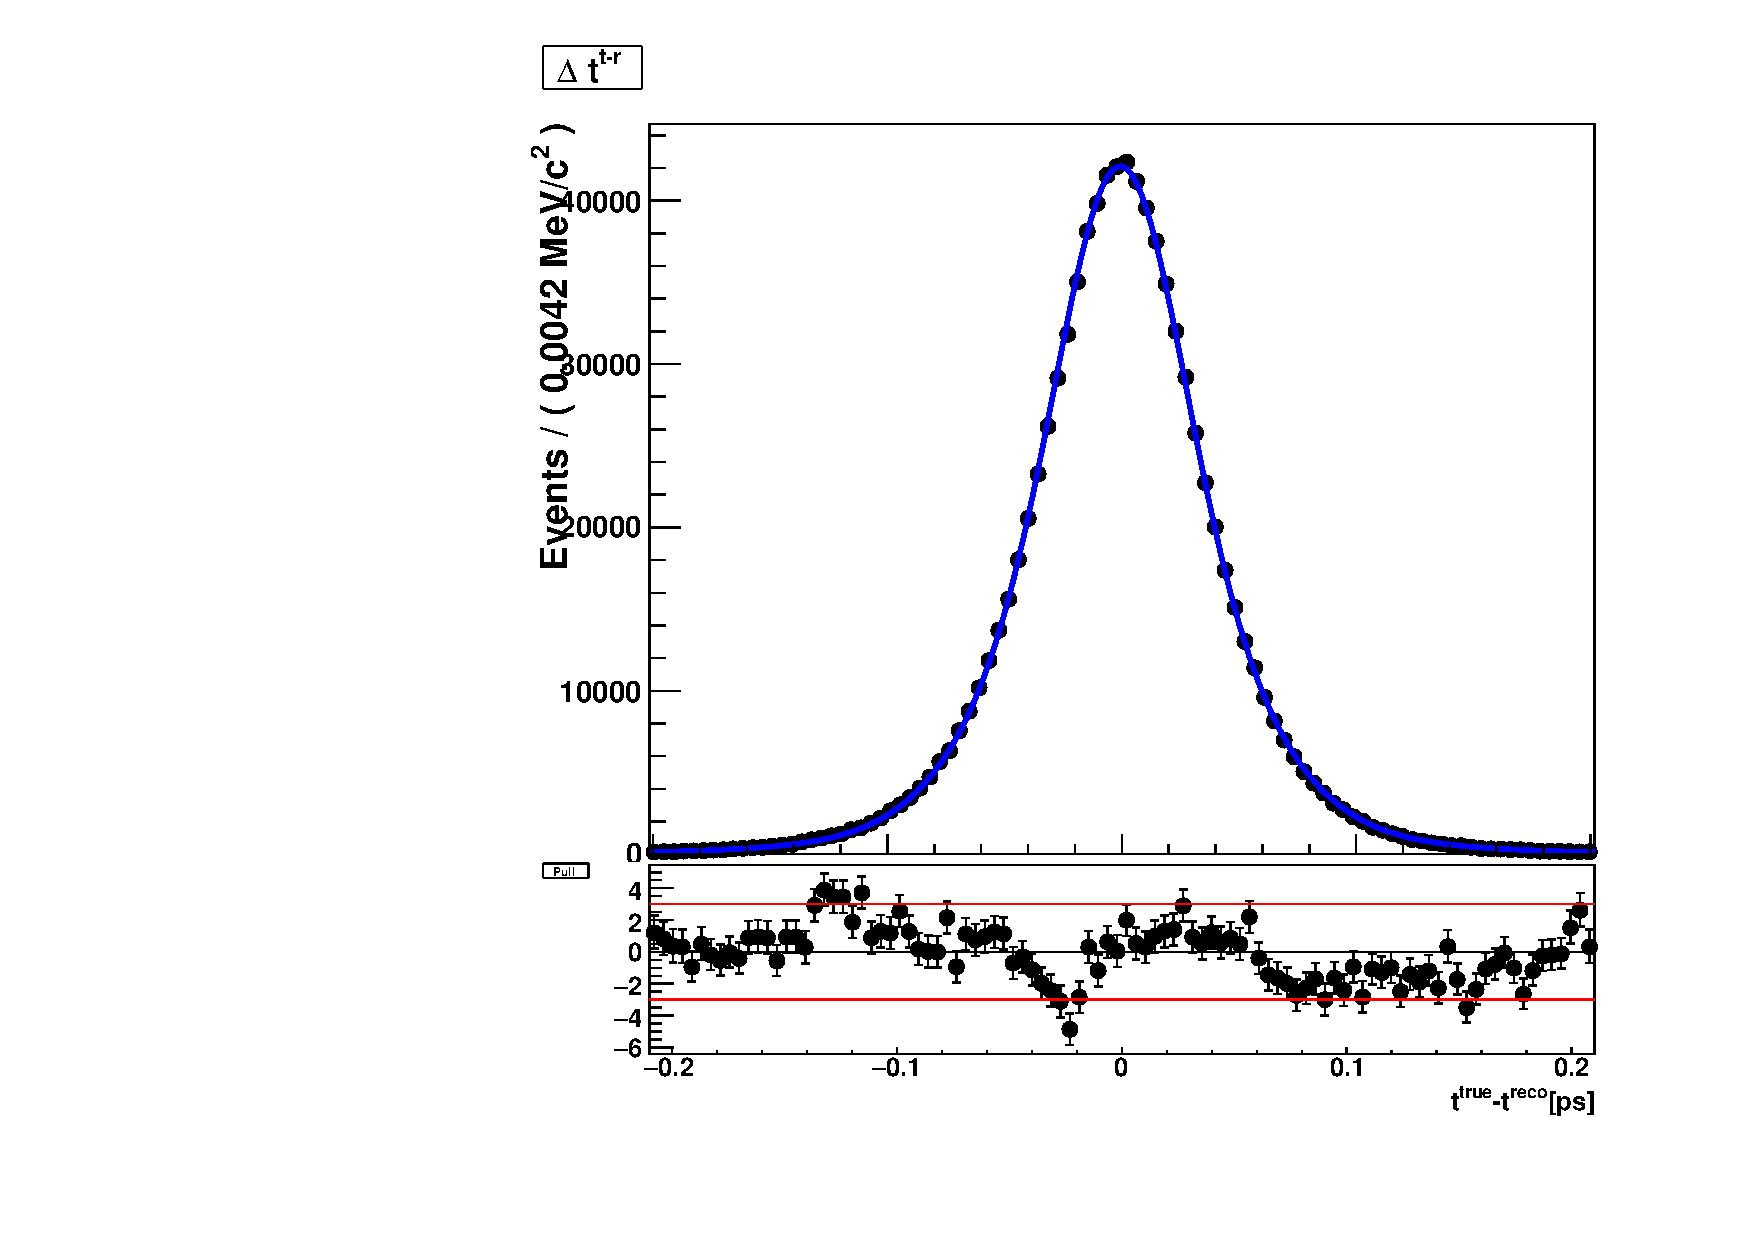
\includegraphics[width=0.49\linewidth]{TimeRes/time_diff_ps_MC12_Bs2JpsiMuMuPhi_unbias_pull.pdf}\put(-115,-4){(b)}
  \end{center}
  \caption{
   The distribution of $t = t^{true} - t^{reco}$ of 2012 simulated (a) $\Bs\to\jpsi(\epem)\phi$ and (b) $\Bs\to\jpsi(\mumu)\Kp\Km$ data samples. The solid blue line shows the result of a fit of the triple Gaussian resolution model. The black points with error bars represent data.
}
  \label{fig:TimeResMC12}
\end{figure}
\begin{table}[htb]
  \caption{
    The resolution model parameters obtained from a fit to the difference between the true and reconstructed decay time using 2012 simulated $\Bs\to\jpsi(\epem)\phi$ and $\Bs\to\jpsi(\mumu)\Kp\Km$ data samples.
}
\small{
\begin{center} \begin{tabular}{ccc}
    \hline
    & $\Bs\to\jpsi(\epem)\phi$ & $\Bs\to\jpsi(\mumu)\Kp\Km$  \\
    \hline
   $\mu_{\text{Gaussians}}$~[$\ps$] & 0.00010$\pm$0.00012 & -0.000656$\pm$0.00004  \\
   $\sigma_{1}$~[$\ps$]& 0.0836$\pm$0.0022 & 0.0249$\pm$0.0004  \\
   $\sigma_{2}$~[$\ps$]& 0.0243$\pm$0.0017 & 0.0871$\pm$0.0017 \\
   $\sigma_{3}$~[$\ps$]& 0.0416$\pm$0.0016 & 0.0437$\pm$0.0006 \\
   f$_{1}$ & 0.194$\pm$0.018 & 0.340$\pm$0.017 \\
   f$_{2}$ & 0.207$\pm$0.053 & 0.099$\pm$0.007 \\
   f$_{3}$ & 0.599$\pm$0.050 & 0.561$\pm$0.017 \\
   \hline
   $\sigma_{eff}$~[ps] & 0.0502$\pm$0.0019 & 0.0451$\pm$0.0008  \\
  \hline
    \end{tabular}\end{center}
  }
\label{tab:TimeRes}
\end{table}
\clearpage

\section{Decay time acceptance}\label{sec:TimeAcc}

 As the decay time is used in the log-likelihood fit to data, it is necessary to model the acceptance effects of the detector and selection process. To perform this we use the data driven {\tt TISTOS} method to determine the trigger efficiencies in data and simulation. The detailed procedure of the {\tt TISTOS} method is described in Ref.~\cite{LHCb:PUB-2014-039} but the main concept is repeated in this paper. 
 
 In the LHCb, the efficiency (conventionally) is a product of three terms:
 \begin{equation}
  \epsilon_{tot} = \epsilon_{rec|acc}\cdot\epsilon_{sel|rec}\cdot\epsilon_{trig|sel},
 \end{equation}
 where the particles in the candidate events must first lie within the detector acceptance, then be reconstructed, selected, and finally passed the trigger requirements. The trigger efficiency is defined on the final sample of selected events:
 \begin{equation}\label{eq:TrigEff}
  \epsilon_{trig}\equiv\epsilon_{trig|sel}\equiv\frac{N_{trig}}{N_{sel}}.
 \end{equation}
 To estimate the trigger efficiency (Eq.~\ref{eq:TrigEff}) from the data, the events are splitted into two trigger categories:
 \begin{itemize}
  \item Triggered On Signal (TOS): events for which the presence of the signal is sufficient to generate a positive trigger decision;
  \item Triggered Independent of Signal (TIS): the "rest" of the events is sufficient to generate a positive trigger decision, where the rest of the event is defined through an operational procedure consisting in removing the signal and all detector hits beloning to it.
 \end{itemize}
A single event can be also simultaneously TIS and TOS (TISTOS). If both the presence of the signal alone as well as the rest of the event alone are sufficient to generate a positive trigger decision. Using these event categories, the partial efficiencies are defined as
\begin{equation}\label{eq:PartTrigEff}
 \epsilon_{TOS}\equiv\frac{N_{TOS}}{N_{sel}},\qquad\epsilon_{TIS}\equiv\frac{N_{TIS}}{N_{sel}},\qquad\epsilon_{TISTOS}\equiv\frac{N_{TISTOS}}{N_{sel}}.
\end{equation}

Since the trigger efficiency (Eq.~\ref{eq:TrigEff}) can be expressed using the trigger categories (Eq.~\ref{eq:PartTrigEff}), we express $\epsilon_{trig}$ as follows:
\begin{equation}
 \epsilon_{trig}=\frac{N_{trig}}{N_{sel}}=\frac{N_{trig}}{N_{TIS}}\times\frac{N_{TIS}}{N_{sel}}=\frac{N_{trig}}{N_{TIS}}\times\epsilon_{TIS}.
\end{equation}
That the TIS efficiency of any subsample of the triggered events is the same as that of the whole sample of selected events, it can thus be measured on the TOS sample:
\begin{equation}
 \epsilon_{TIS}\equiv\epsilon_{TIS|TOS}.
\end{equation}
The trigger efficiency can now be expressed as
\begin{equation}\label{eq:FinalTrigEff}
 \epsilon_{trig}=\frac{N_{trig}}{N_{TIS}}\times\frac{N_{TISTOS}}{N_{TOS}},
\end{equation}
where all four quantities can be directly measured from data.

 The trigger efficiencies of the $\Bs\to\jpsi\phi$ data and simulated sample are obtained for two trigger categories (described in Sec.~\ref{subsec:Trigger}):
 \begin{enumerate}
  \item Unbiased: {\tt L0ElectronDecision$\_$TOS} or {\tt L0HadronDecision$\_$TOS}
  \item Biased: {\tt Hlt1TrackAllL0Decision$\_$TOS}
 \end{enumerate}
 In case of biased triggers, the one trigger is chosen since it holds a maximum number of selected events in the whole biased category: 98.4$\%$ of data events and 91.3$\%$ of simulated events.
 
 The $\Bs\to\jpsi\phi$ trigger efficiencies for unbiased and biased triggers are shown in Fig.~\ref{fig:TimeAccTISTOS}.
   \begin{figure}[hbt]
  \begin{center}
    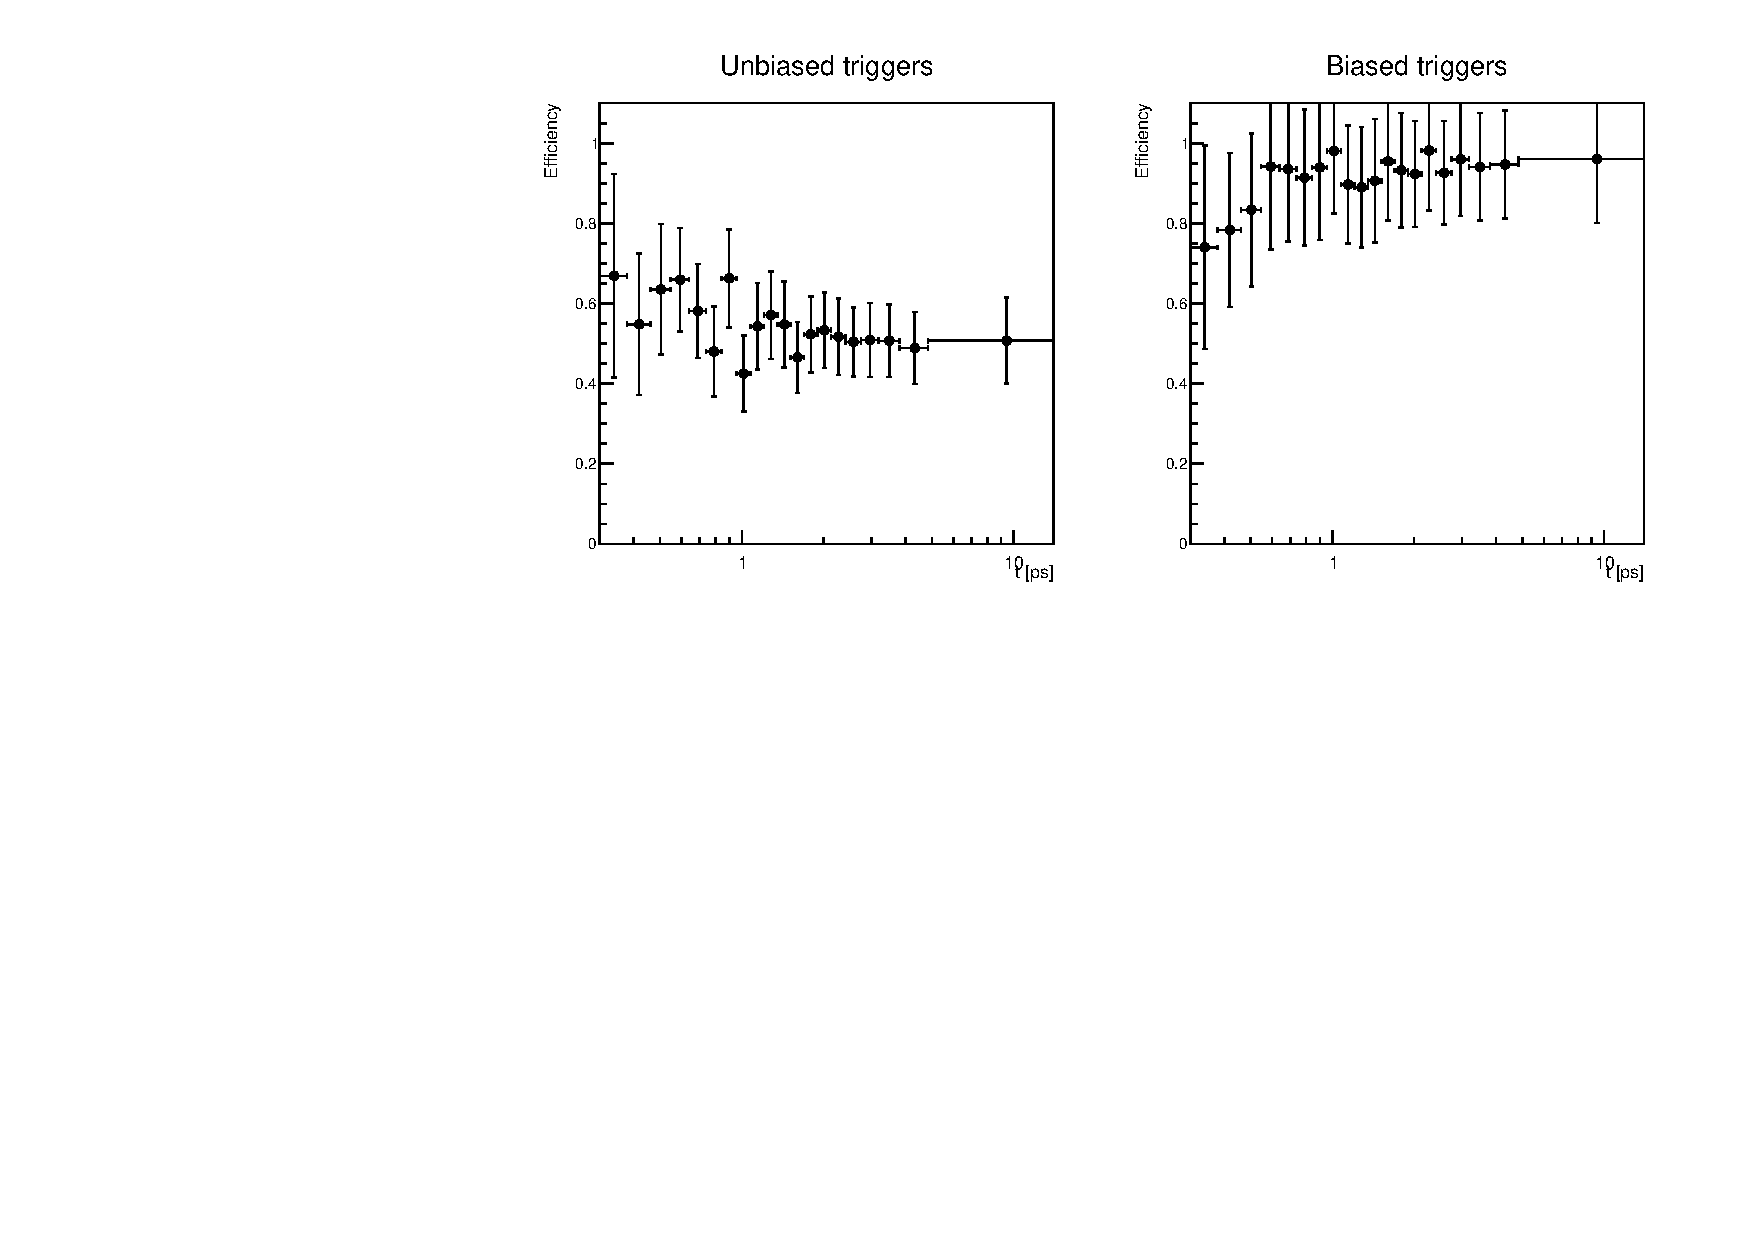
\includegraphics[width=0.9\linewidth]{TimeAcc_TISTOS/Eff_unbL0E_bias_log_data.pdf}\\ 
    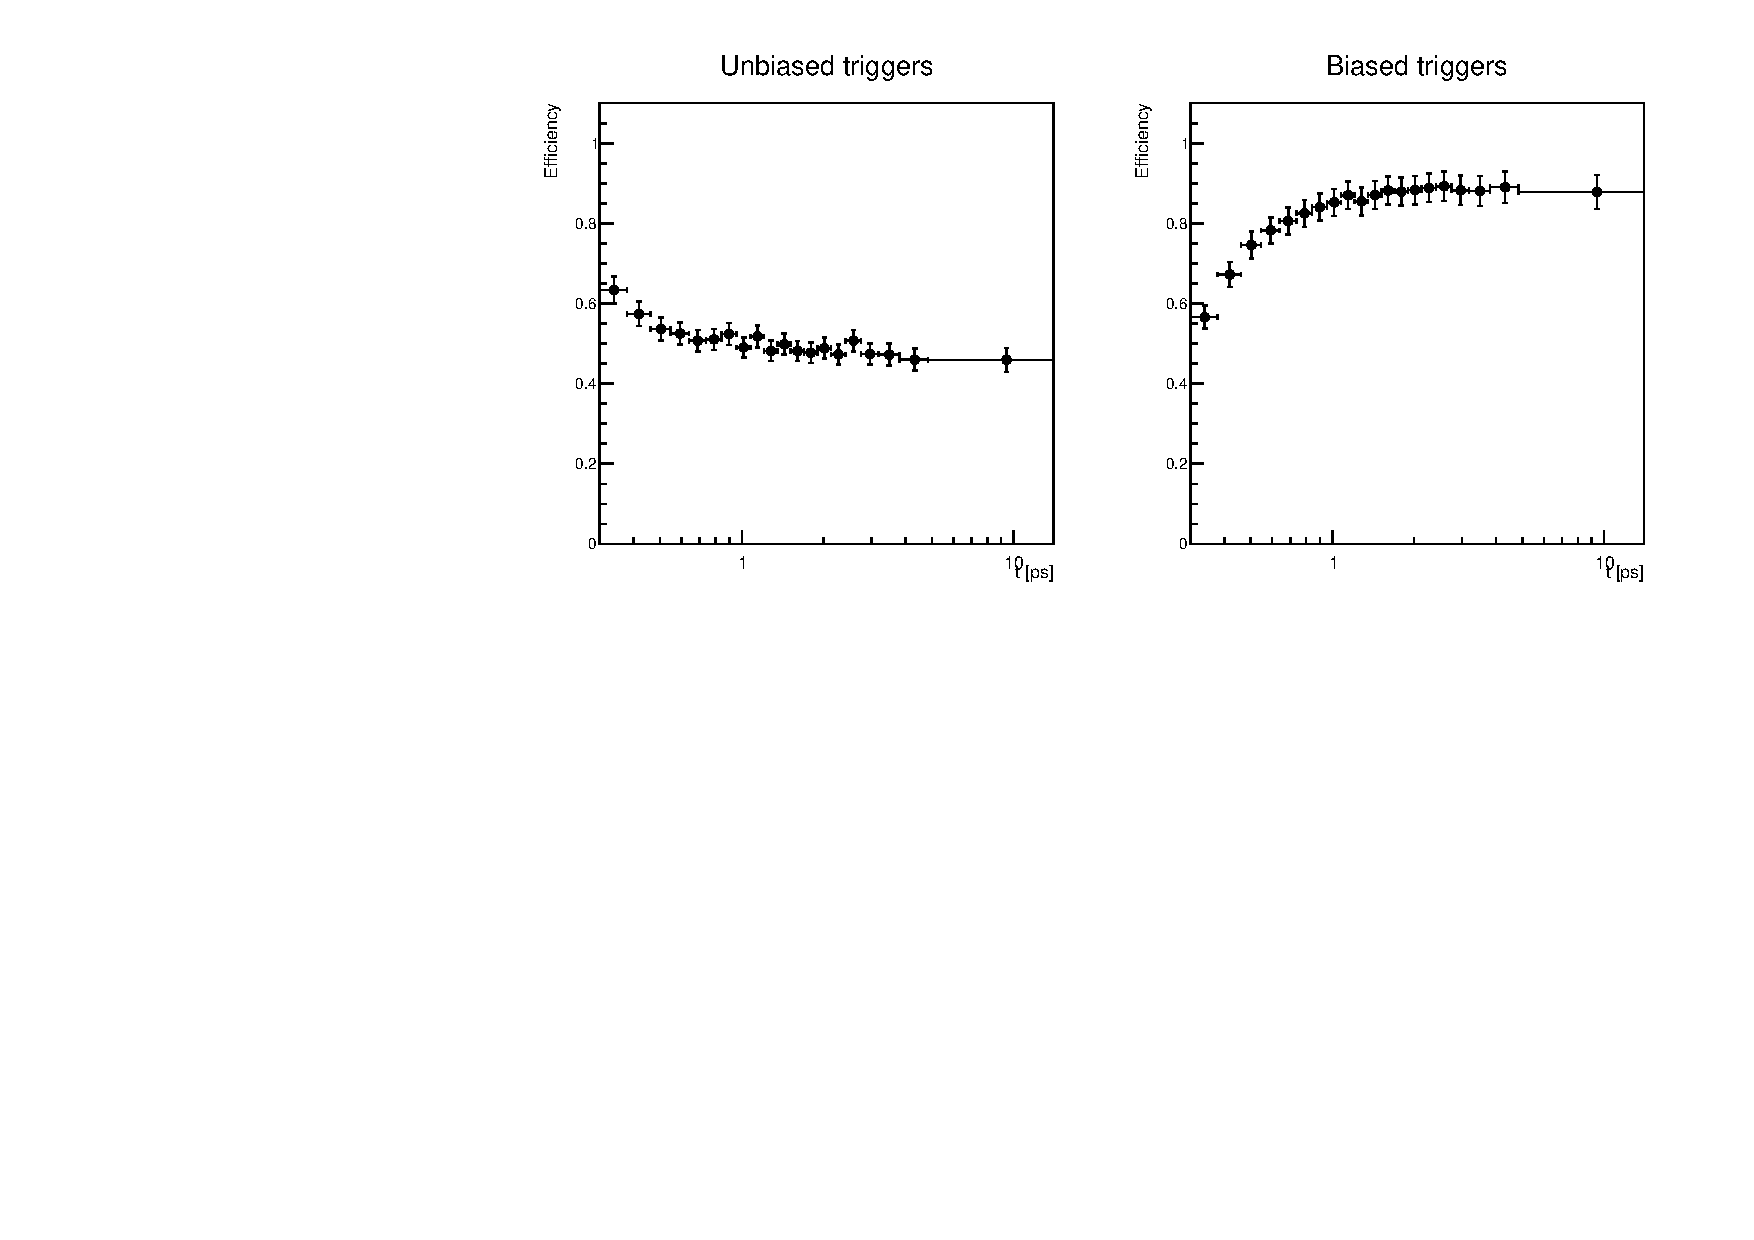
\includegraphics[width=0.9\linewidth]{TimeAcc_TISTOS/Eff_unbL0E_bias_log_MC.pdf}
  \end{center}
  \caption{
  The trigger efficiencies of sWeighted $\Bs\to\jpsi\phi$ data (top) and simulation (bottom) for unbiased (left) and biased (right) triggers depending on the decay time. 
}
  \label{fig:TimeAccTISTOS}
\end{figure}
 
 
 \subsection{Track reconstruction efficiency}\label{subsec:TrackRecEff}
 
 The track reconstruction efficiency is computed as the ratio of the decay time distributions of fully unbiased and truth matched 2012 simulated sample to the toy dataset generated with the 2012 MC physics parameters. The resulting histogram is shown in Fig.~\ref{fig:TimeAccTrackRecEff}. The efficiency ratio is fitted with a quadratic function, $N(1+\beta t+\gamma t^{2})$. The obtained fit parameters of the track reconstruction efficiency for $\Bs\to\jpsi(\epem)\phi$ and $\Bs\to\jpsi(\mumu)\Kp\Km$~\cite{Aaij:2014-039} decays are listed in Table~\ref{tab:TRackRecEff}.
 
  \begin{figure}[hbt]
  \begin{center}
    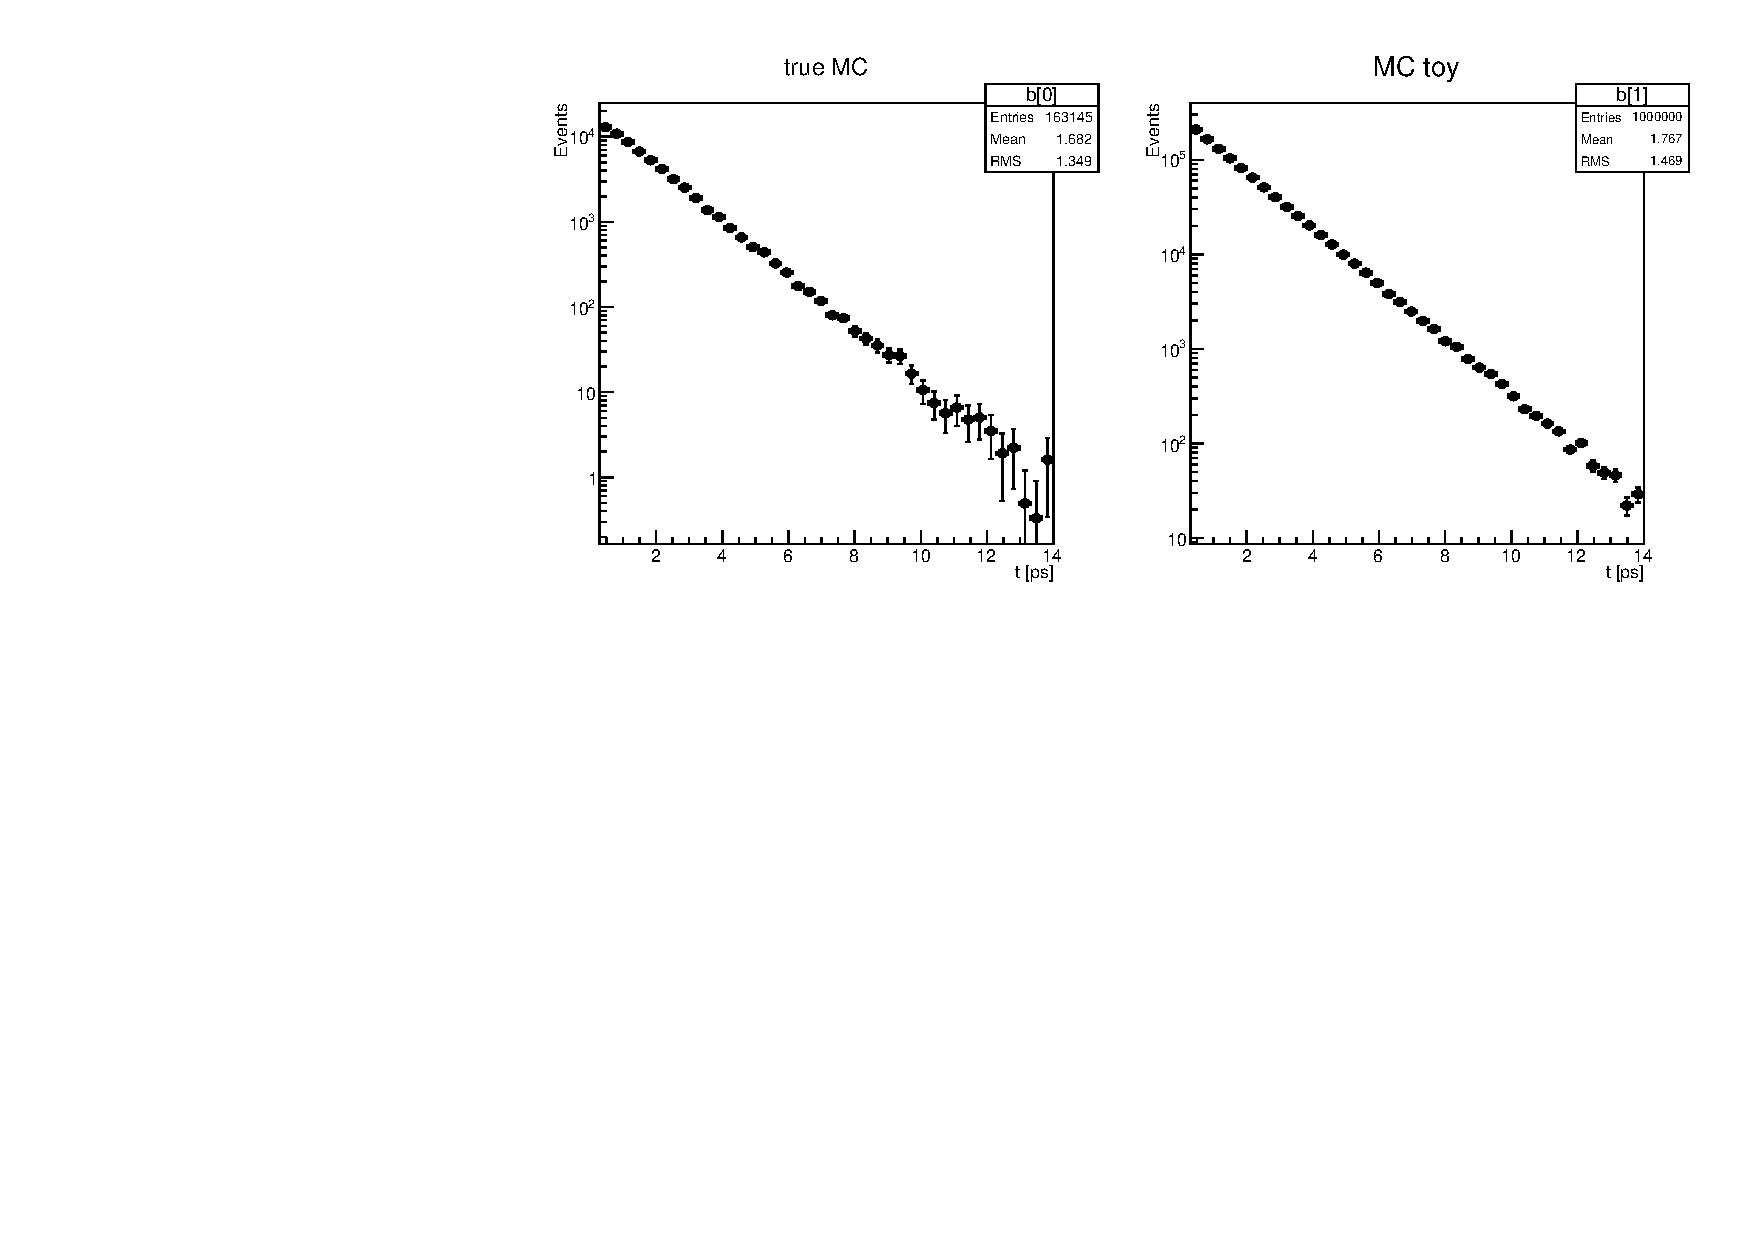
\includegraphics[width=0.9\linewidth]{TimeAcc_high/Time_MCtrue_MCtoy.pdf}\\ 
    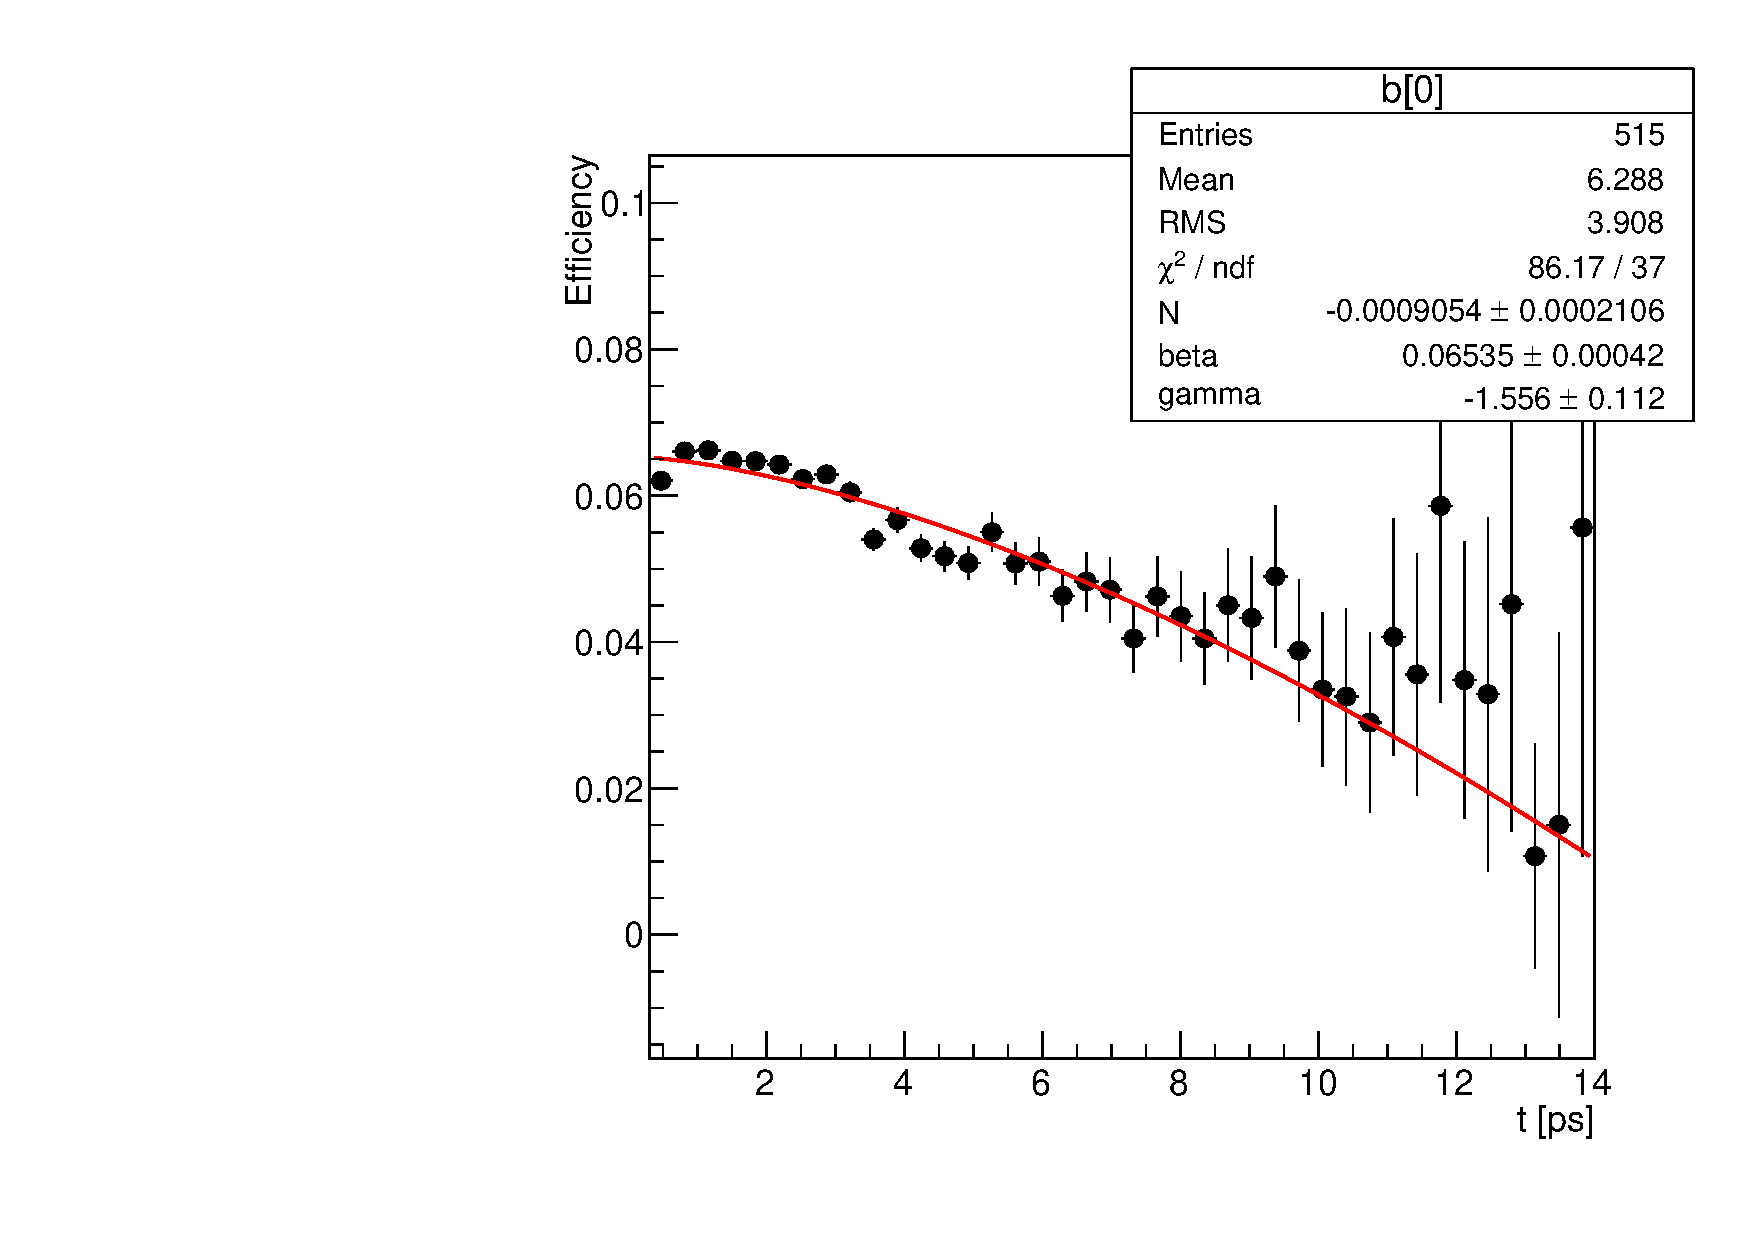
\includegraphics[width=0.45\linewidth]{TimeAcc_high/Efficiency.pdf}
  \end{center}
  \caption{
  The ratio (bottom) of decay time distributions of completely unbiased and truth matched events in 2012 MC (top left) to toy events generated with the 2012 MC physics parameters (top right).
}
  \label{fig:TimeAccTrackRecEff}
\end{figure}

\begin{table}[htb]
  \caption{
    The fit parameters of the track reconstruction efficiency for $\Bs\to\jpsi(\epem)\phi$ and $\Bs\to\jpsi(\mumu)\Kp\Km$ decays.}
    \small{
\begin{center}\begin{tabular}{c|c|c}
   \hline
   Parameter & $B^{0}_{s}\rightarrow J/\psi(e^{+}e^{-})\phi$ & $B^{0}_{s}\rightarrow J/\psi(\mu^{+}\mu^{-})K^{+}K^{+}$ \\
  \hline
   $N_{evt}$ & 515 & 8 241\\
   $\mu$ & 6.29 & 6.59\\
   RMS & 3.91 & 3.82\\
   $\chi^{2}$/ndf & 86.17/37 & 50.16/47\\
   N & -0.00091$\pm$0.00021 & 0.09722$\pm$0.00023\\
   $\beta$ & 0.06535$\pm$0.00042 & 0.00320$\pm$0.00183\\
   $\gamma$&-1.556$\pm$0.112 & -0.00227$\pm$0.00025\\
   \hline
    \end{tabular}
   \end{center}
  }
\label{tab:TRackRecEff}
\end{table}
\clearpage

\section{Angular acceptance}\label{sec:AngAcc}

Effects of angular acceptance are modeled with normalization weights (see Ref.~\cite{Aaij:2012-067}, Sec.~3.3). The normalization weights are obtained from fully simulated signal sample from the Sim08 production (Sec.~\ref{subsec:MC}), as described in Sec.~\ref{subsec:NormWeightMC}. 

\subsection{Normalization weights from full simulation}\label{subsec:NormWeightMC}
 The angular acceptance normalization weights determined with the Sim08 Monte Carlo samples are shown in Table~\ref{tab:UnccorrAngAccMCfull}. Table~\ref{tab:UnccorrAngAccMCfullCorrMatrix} shows the correlations between the errors of the weights. In Table~\ref{tab:UnccorrAngAcc} the 10 weights corresponding to 10 terms of the PDF (Eq.~\ref{eq:decayrate}) are split by running year. As no significant difference is observed between the two years (Fig.~\ref{fig:AnglesAccMC11MC12}), the weights are calculated and normalized separately for each running year and then they are combined to the one final set of weights of Table~\ref{tab:UnccorrAngAccMCfull}. The one-dimentional projections of the angular efficiency functions are shown in Fig.~\ref{fig:AnglesAccMCfull}. No reweighting of the final state kinematics has been applied since the $\Bs$ and $K$ momentum and $\Kp\Km$ mass distribution in simulation are observed to well reproduce those in data (Fig.~\ref{fig:AnglesAcc_IterMeth}).


 \begin{table}[htb]
  \caption{
    The uncorrected angular acceptance weights for the sum of 2011 and 2012 Sim08 simulated sample.}
    \small{
\begin{center}\begin{tabular}{ccc}
    \hline
   & k & $\xi_{k}/\xi_{1}$   \\
    \hline
  1 & (00) & 0.9796$\pm$0.0010 \\
  2 & ($\parallel\parallel$) & 1.0206$\pm$0.0012\\
  3 & ($\perp\perp$) & 1.0208$\pm$0.0012\\
  4 & ($\parallel\perp$) & 0.0005$\pm$0.0013\\
  5 & (0$\parallel$) & 0.0007$\pm$0.0009\\
  6 & (0$\perp$) & 0.0014$\pm$0.0009\\
  7 & (SS) & 0.9929$\pm$0.0008\\
  8 & (S$\parallel$) & 0.0002$\pm$0.0012\\
  9 & (S$\perp$) & -0.0003$\pm$0.0012\\
  10 & (S0) & -0.0038$\pm$0.0027\\
  \hline
    \end{tabular}\end{center}
  }
\label{tab:UnccorrAngAccMCfull}
\end{table}

 \begin{table}[htb]
  \caption{
    The correlations between the uncorrected angular acceptance weights for the sum of 2011 and 2012 Sim08 simulated sample.
}
    \small{
\begin{center}\begin{tabular}{ccccccccccc}
    \hline
   k & 1(00) & 2($\parallel\parallel$)&3($\perp\perp$)&4($\parallel\perp$)&5(0$\parallel$)&6(0$\perp$)&7(SS)&8(S$\parallel$)&9(S$\perp$)&10(S0)   \\
    \hline
  1(00) & 1  & -0.67 & -0.69 & & 0.27 & & -0.05 & & &\\
  2($\parallel\parallel$) & & 1 & 0.40 & & 0.21 & & 0.24 & & &\\
  3($\perp\perp$) & & & 1 & & 0.31 & & 0.18 & & &\\
  4($\parallel\perp$) & & & & 1 & & -0.09 & & & & \\
  5(0$\parallel$) & & & & & 1 & & 0.30 & & &\\
  6(0$\perp$) & & & & & & 1 & & & & \\
  7(SS) & & & & & & & 1 & & &\\
  8(S$\parallel$) & & & & & & & & 1 & & 0.14\\
  9(S$\perp$) & & & & & & & & & 1 & \\
  10(S0) & & & & & & & & & & 1\\
  \hline
    \end{tabular}\end{center}
  }
\label{tab:UnccorrAngAccMCfullCorrMatrix}
\end{table}

 \begin{table}[htb]
  \caption{
    The uncorrected angular acceptance weights for the 2011 and 2012 Sim08 simulated samples.}
    \small{
\begin{center}\begin{tabular}{ccccc}
    \hline
   & & Sim08 2011 & Sim08 2012 & \\ 
   & k & $\xi_{k}/\xi_{1}$ & $\xi_{k}/\xi_{1}$ & Diff($\sigma$) \\
    \hline
  1 & (00) & 0.9803$\pm$0.0014 &0.9786$\pm$0.0015 & -0.8\\
  2 & ($\parallel\parallel$) & 1.0197$\pm$0.0017& 1.0219$\pm$0.0019 & +0.9\\
  3 & ($\perp\perp$) & 1.0203$\pm$0.0016& 1.0214$\pm$0.0018 & +0.5\\
  4 & ($\parallel\perp$) & 0.0013$\pm$0.0018& -0.0005$\pm$0.0020 & +0.7\\
  5 & (0$\parallel$) & 0.0008$\pm$0.0012& 0.0004$\pm$0.0014 & -0.2\\
  6 & (0$\perp$) & 0.0017$\pm$0.0012& 0.0011$\pm$0.0013 & -0.3\\
  7 & (SS) & 0.9909$\pm$0.0011& 0.9953$\pm$0.0012 & +2.7\\
  8 & (S$\parallel$) & -0.0018$\pm$0.0016& 0.0025$\pm$0.0018 & +1.8\\
  9 & (S$\perp$) & 0.0006$\pm$0.0016& -0.0013$\pm$0.0018 & -0.8\\
  10 & (S0) & -0.0055$\pm$0.0036& -0.0017$\pm$0.0040 & +0.7\\
  \hline
    \end{tabular}\end{center}
  }
\label{tab:UnccorrAngAcc}
\end{table}

\begin{figure}[hbt]
  \begin{center}
    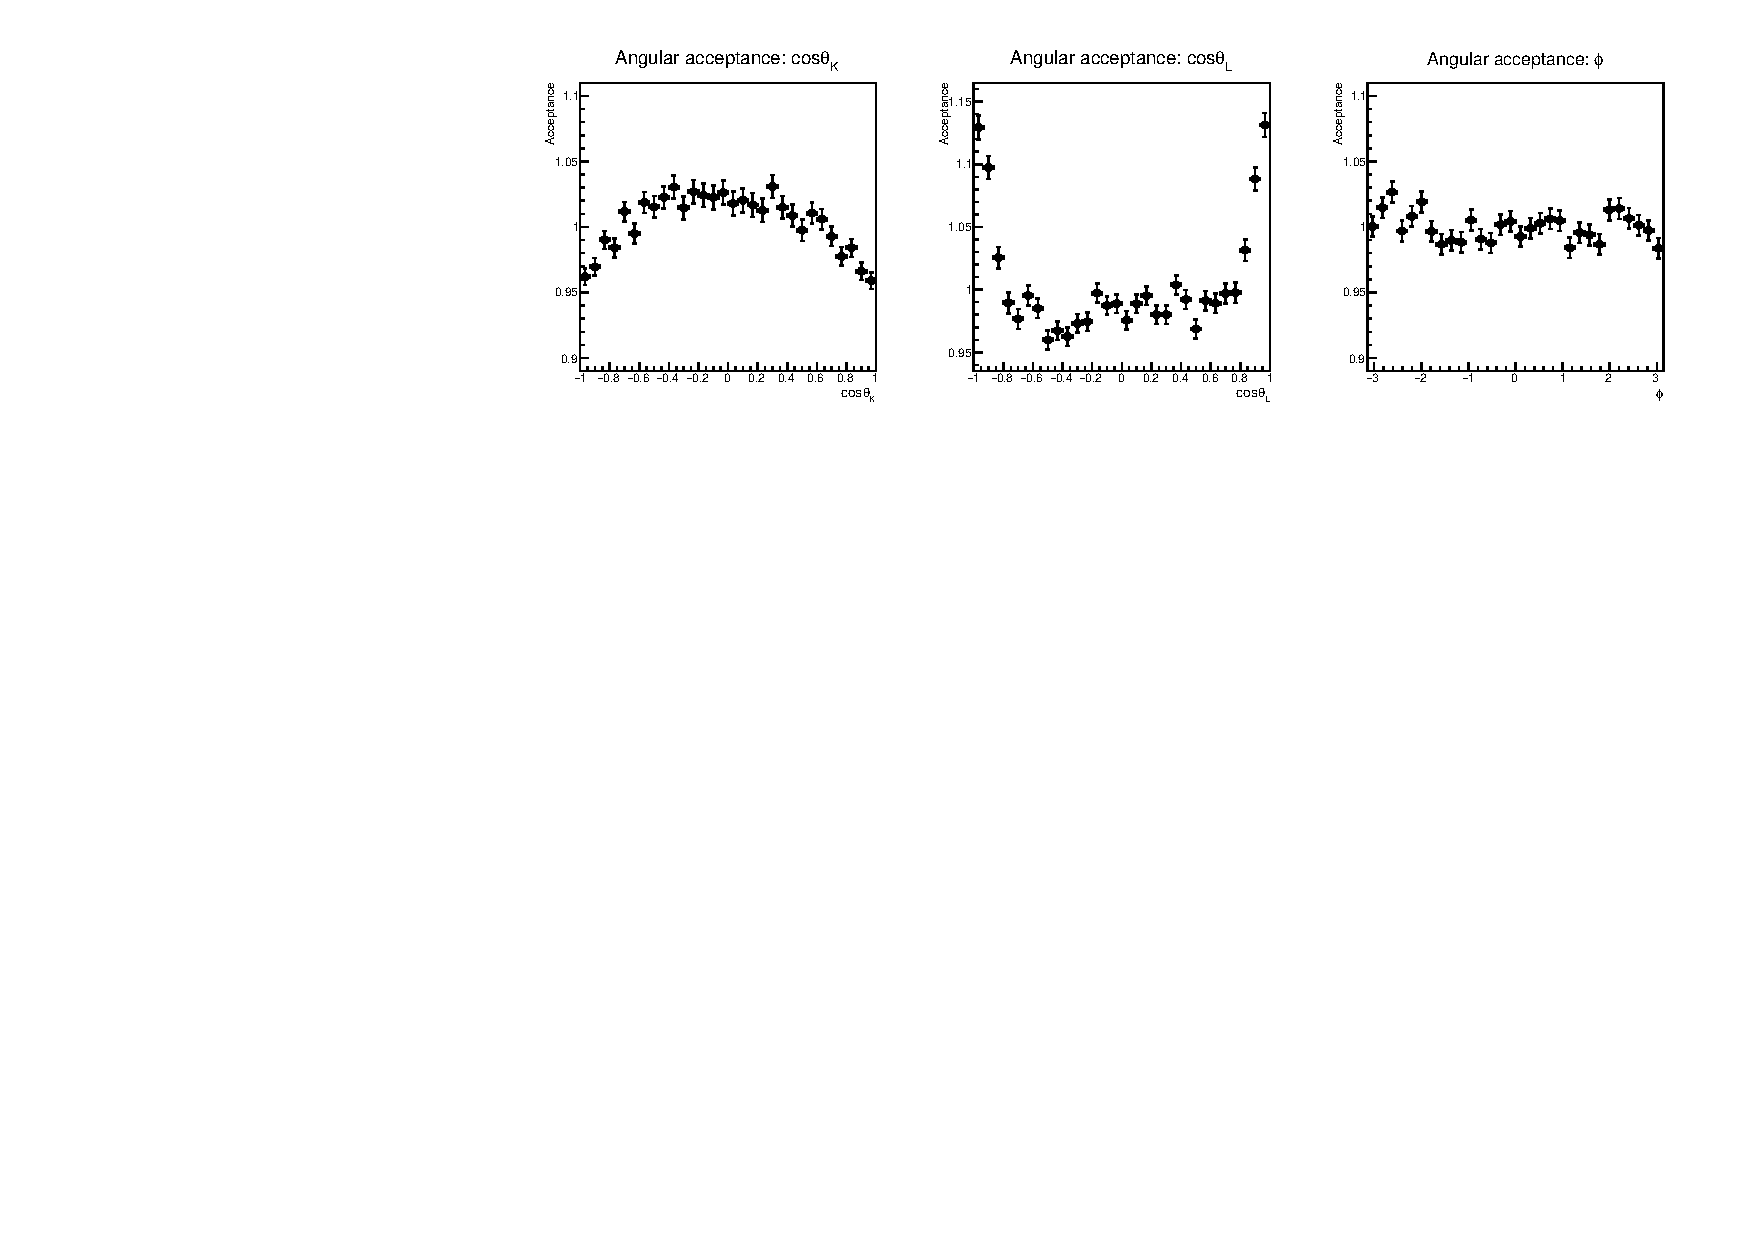
\includegraphics[width=1.05\linewidth]{AnglesAcc/AngAcc_MCfull_TupleBsDetached.pdf}\\
     \vspace*{-0.5cm}
  \end{center}
    \caption{
    The angular acceptance projections as function of the three helicity angles for full simulated $\Bs\to\jpsi(\epem)\phi$ sample.
}
  \label{fig:AnglesAccMCfull} 
\end{figure}

\begin{figure}[hbt]
  \begin{center}
    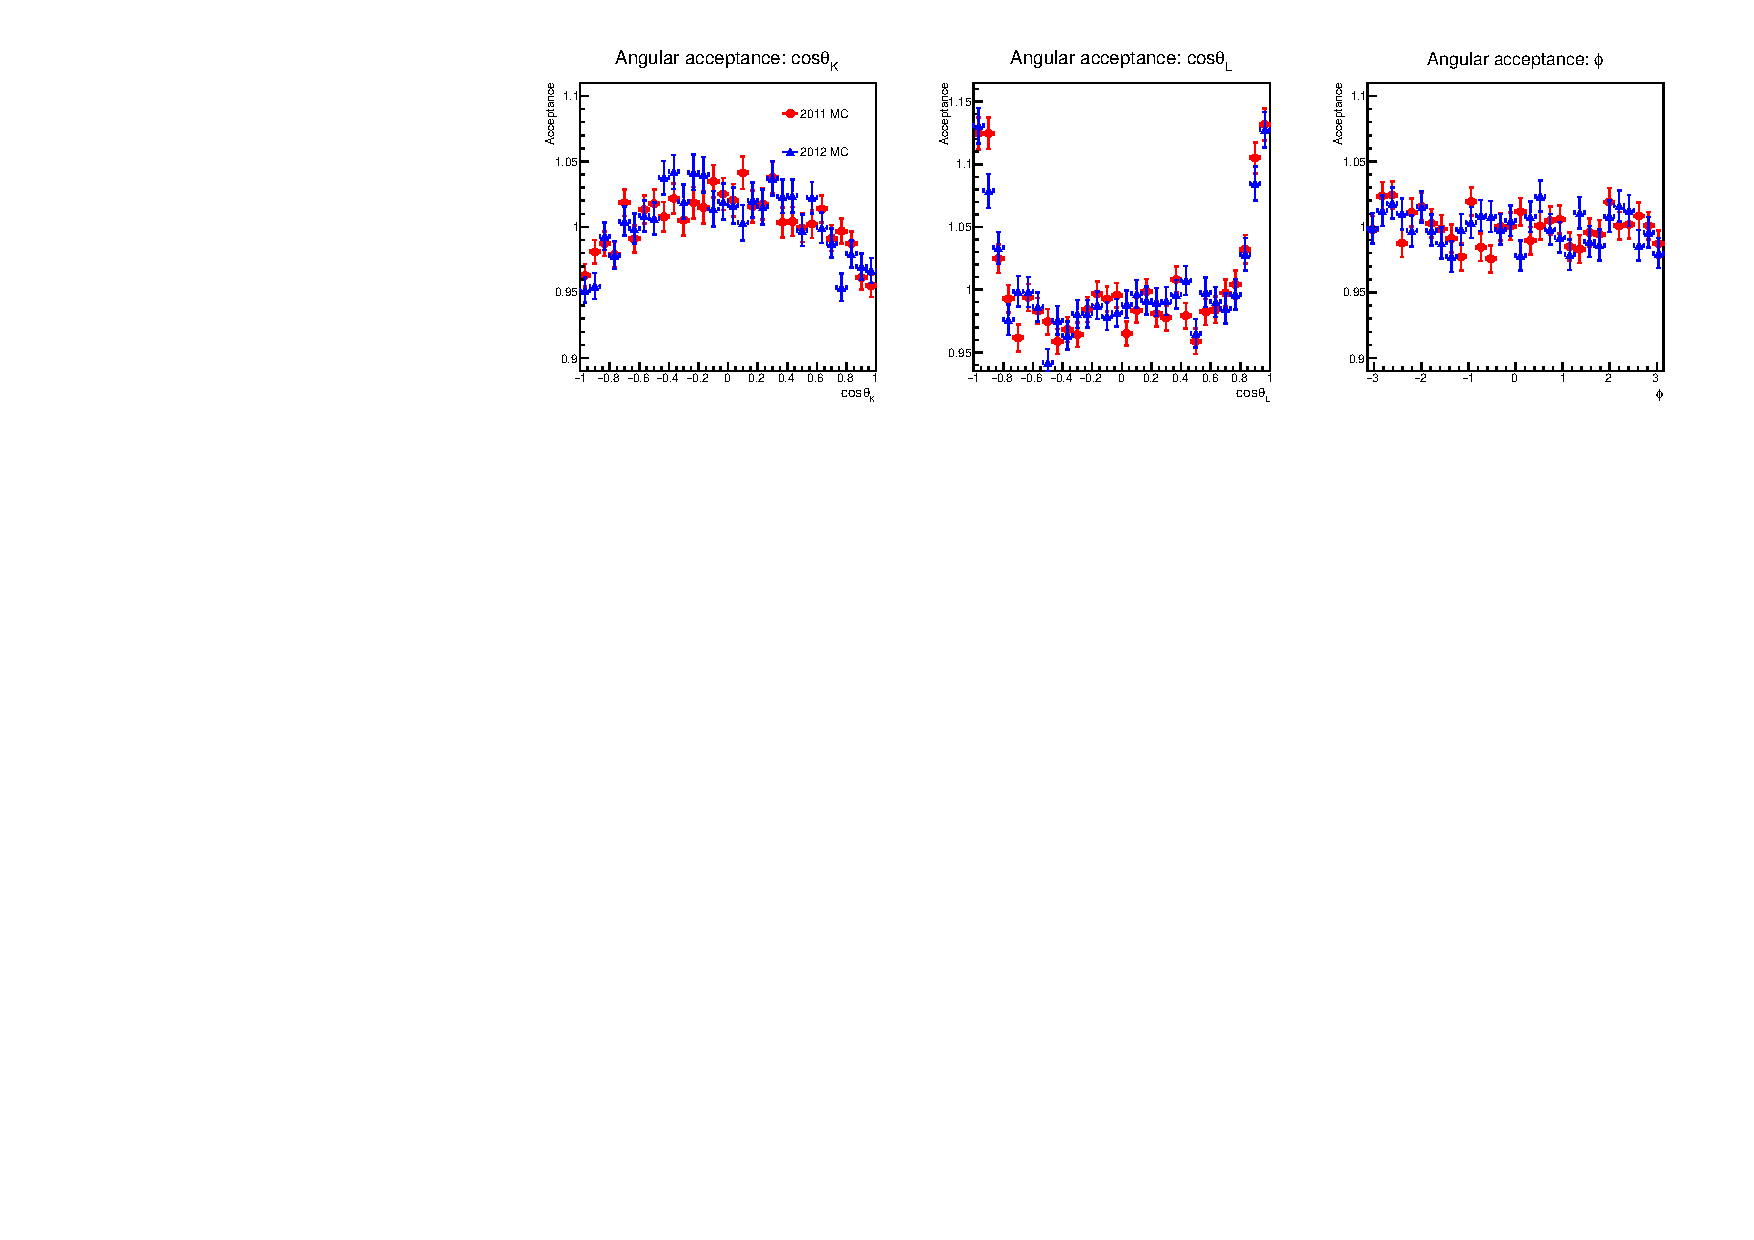
\includegraphics[width=1.05\linewidth]{AnglesAcc/AngAcc_MC11_MC12_TupleBsDetached.pdf}\\
     \vspace*{-0.5cm}
  \end{center}
    \caption{
    The angular acceptance projections as function of the three helicity angles for simulated $\Bs\to\jpsi(\epem)\phi$ events. 2011 and 2012 samples are compared.
}
\label{fig:AnglesAccMC11MC12} 
\end{figure}

\begin{figure}[hbt]
  \begin{center}
    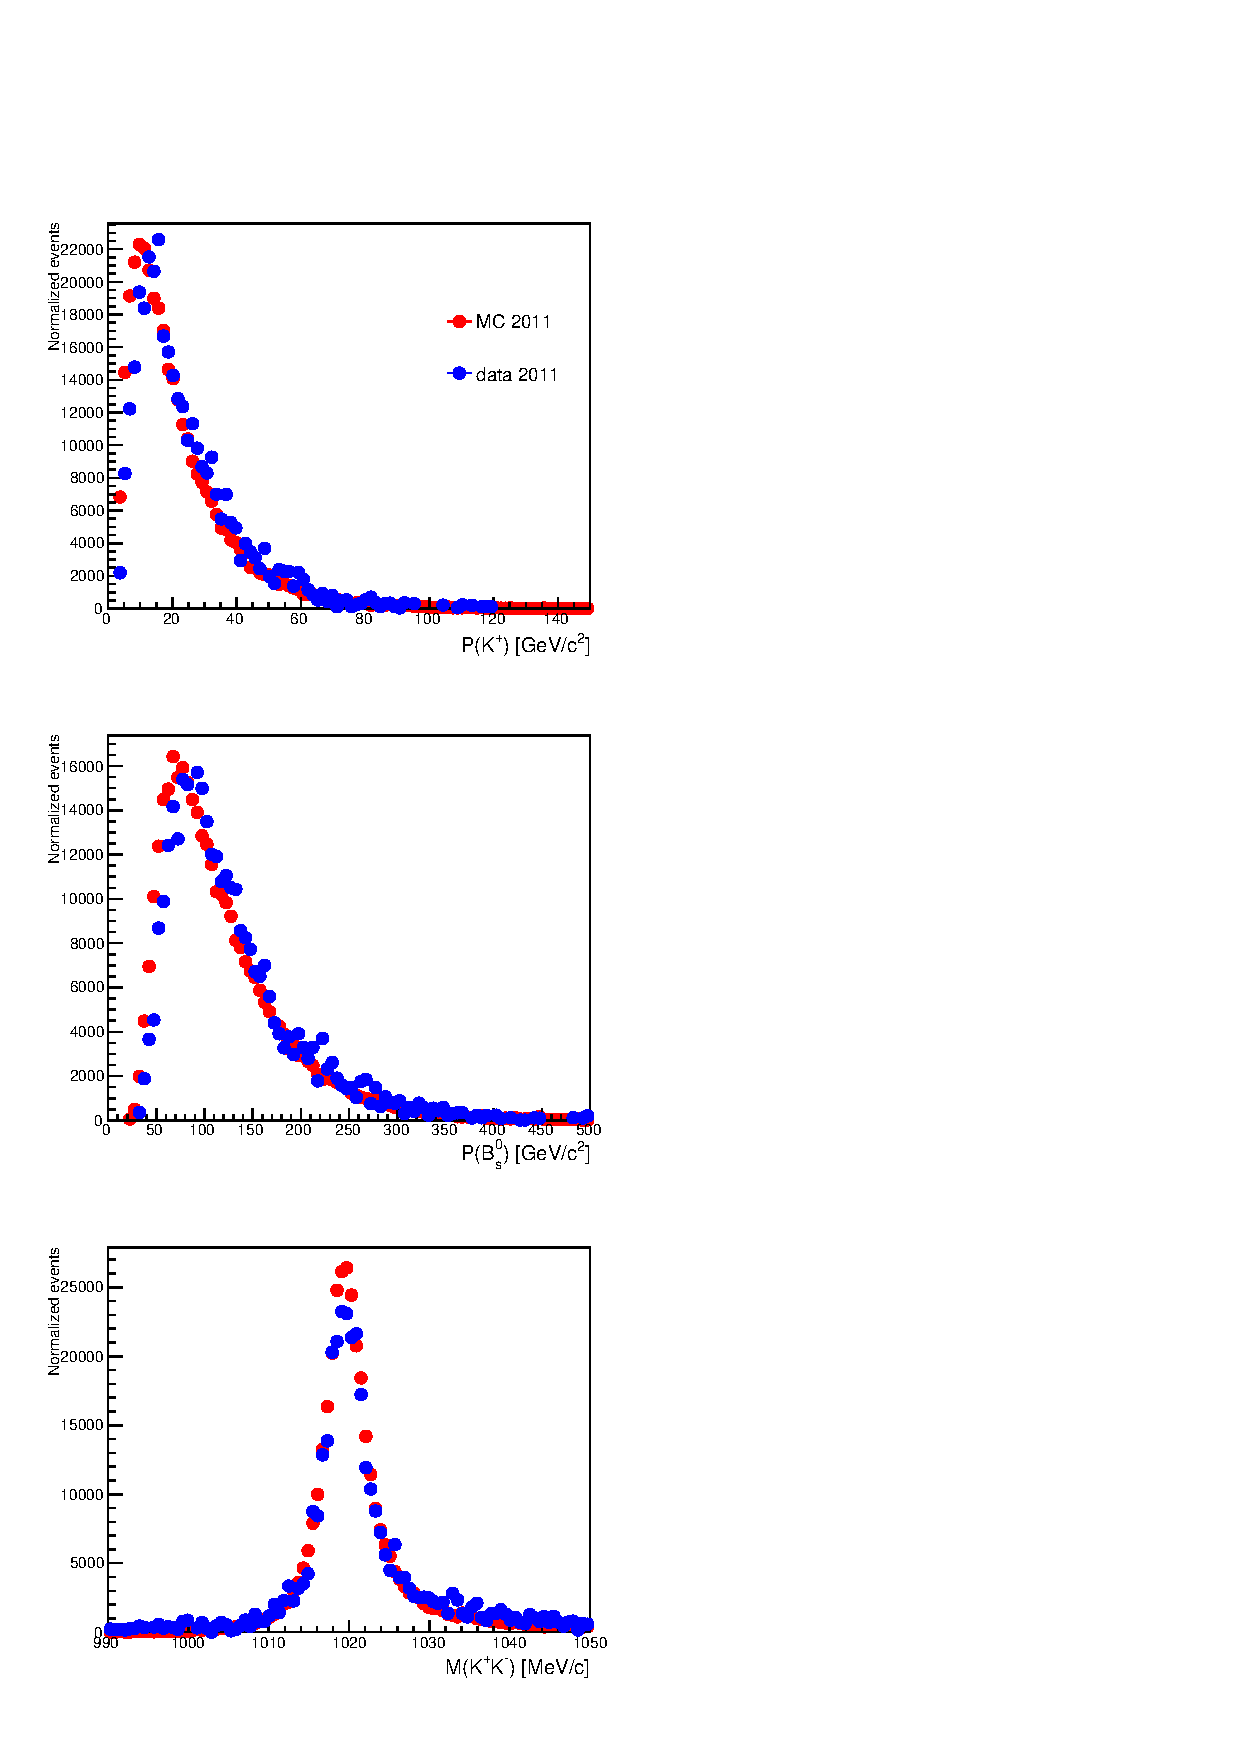
\includegraphics[width=0.48\linewidth]{AnglesAcc/AngAcc_IterMeth11.pdf}
    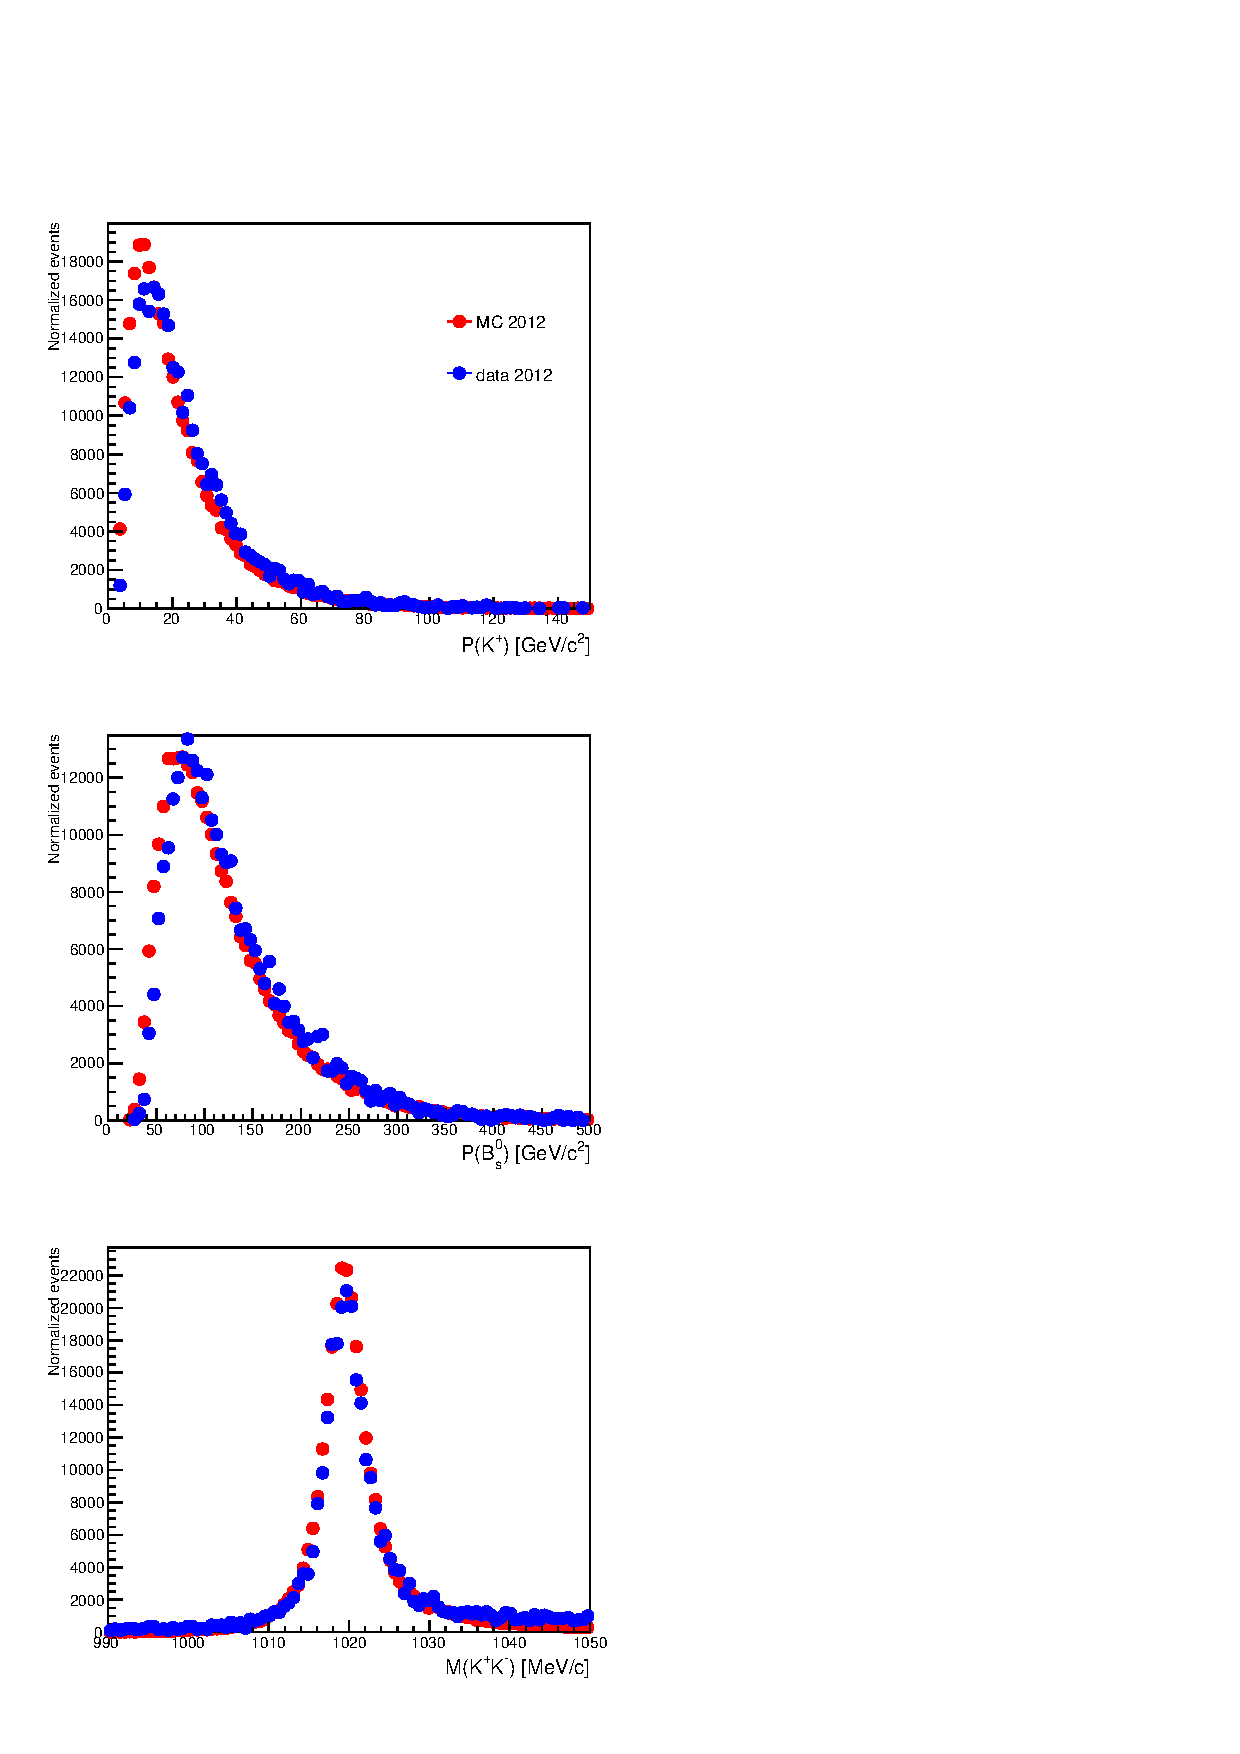
\includegraphics[width=0.48\linewidth]{AnglesAcc/AngAcc_IterMeth12.pdf}
     \vspace*{-0.5cm}
  \end{center}
    \caption{
    The comparison between the kinematical variables of $\Bs\to\jpsi(\epem)\phi$ signal events in sWeighted data (blue) and simulation data (red) for 2011 (left) and 2012 (right) run periods.
}
  \label{fig:AnglesAcc_IterMeth} 
\end{figure}
\clearpage

\section{Angular resolution}\label{sec:AngRes}

The angular resolution is defined as the difference between true and reconstructed angle in simulated sample. The one-dimensional projections of the three angular resolutions are shown in Fig.~\ref{fig:AnglesRes}. For angles $\theta_{K}$ and $\theta_{L}$, the used fitted model is a sum of three Gaussian functions, while for $\phi$ a double Gaussian plus a Voigtian component is required in order to better model the large non-Gaussian tails. The parameters determined from these fits are reported in Table~\ref{tab:AnglesRes}. It has been shown in Ref.~\cite{Aaij:2014-039} that there is no correlation between the resolution of the three angles. Two-dimensional distributions of the helicity angles are shown in Fig.~\ref{fig:AnglesRes2D}. 

Based upon studies performed in Ref.~\cite{Aaij:2014-039}, the effect from the angular resolution is negligible. It is considered as a source of systematic uncertainty in Sec.~\ref{subsec:Syst:AngRes}.

\begin{table}[htb]
  \caption{
    The fit results to the angular resolution distributions for each of the helicity angles taken from $\Bs\to\jpsi(\epem)\phi$ simulated signal sample for 2011 and 2012 run periods. The last row shows the effective Gaussian resolution computed for $\theta_{K}$ and $\theta_{L}$.
}
    \small{
 \begin{center}
  \begin{tabular}{cccc}
   \hline
    & 3 Gaussian & 3 Gaussian & 2 Gaussian+Voigtian\\
  \hline
  Parameter & $\theta_{L}$ &  $\theta_{K}$ &$\phi$\\
  \hline
    $\sigma_{1}$[mrad]  & 20.61$\pm$0.18 &  12.66$\pm$0.06 &  17.35$\pm$0.11 \\
    $\sigma_{2}$[mrad]  & 7.083$\pm$0.08 &  21.42$\pm$0.08 &  36.03$\pm$0.36 \\
    $\sigma_{3}$[mrad]  & 62.54$\pm$0.35 &  47.71$\pm$0.80 &  38.30$\pm$0.77 \\
    $\sigma_{4}$[mrad]  & - &  - &  83.00$\pm$1.20 \\
    $f_{1}$  & 0.3902$\pm$0.0026 &  0.3926$\pm$0.0058 &  0.4970$\pm$0.0073 \\
    $f_{2}$  & 0.1545$\pm$0.0031 &  0.5632$\pm$0.0052 &  0.4027$\pm$0.0056 \\
    $f_{3}$  & 0.4553$\pm$0.0040 &  0.0442$\pm$0.0078 &  0.1003$\pm$0.0091 \\
    \hline
    $\sigma_{eff}$[mrad]  & 44.21$\pm$0.34 &  20.54$\pm$0.45 &  - \\
   \hline
    \end{tabular}
  \end{center}
   }
\label{tab:AnglesRes}
\end{table}

\begin{figure}[hbt]
  \begin{center}
    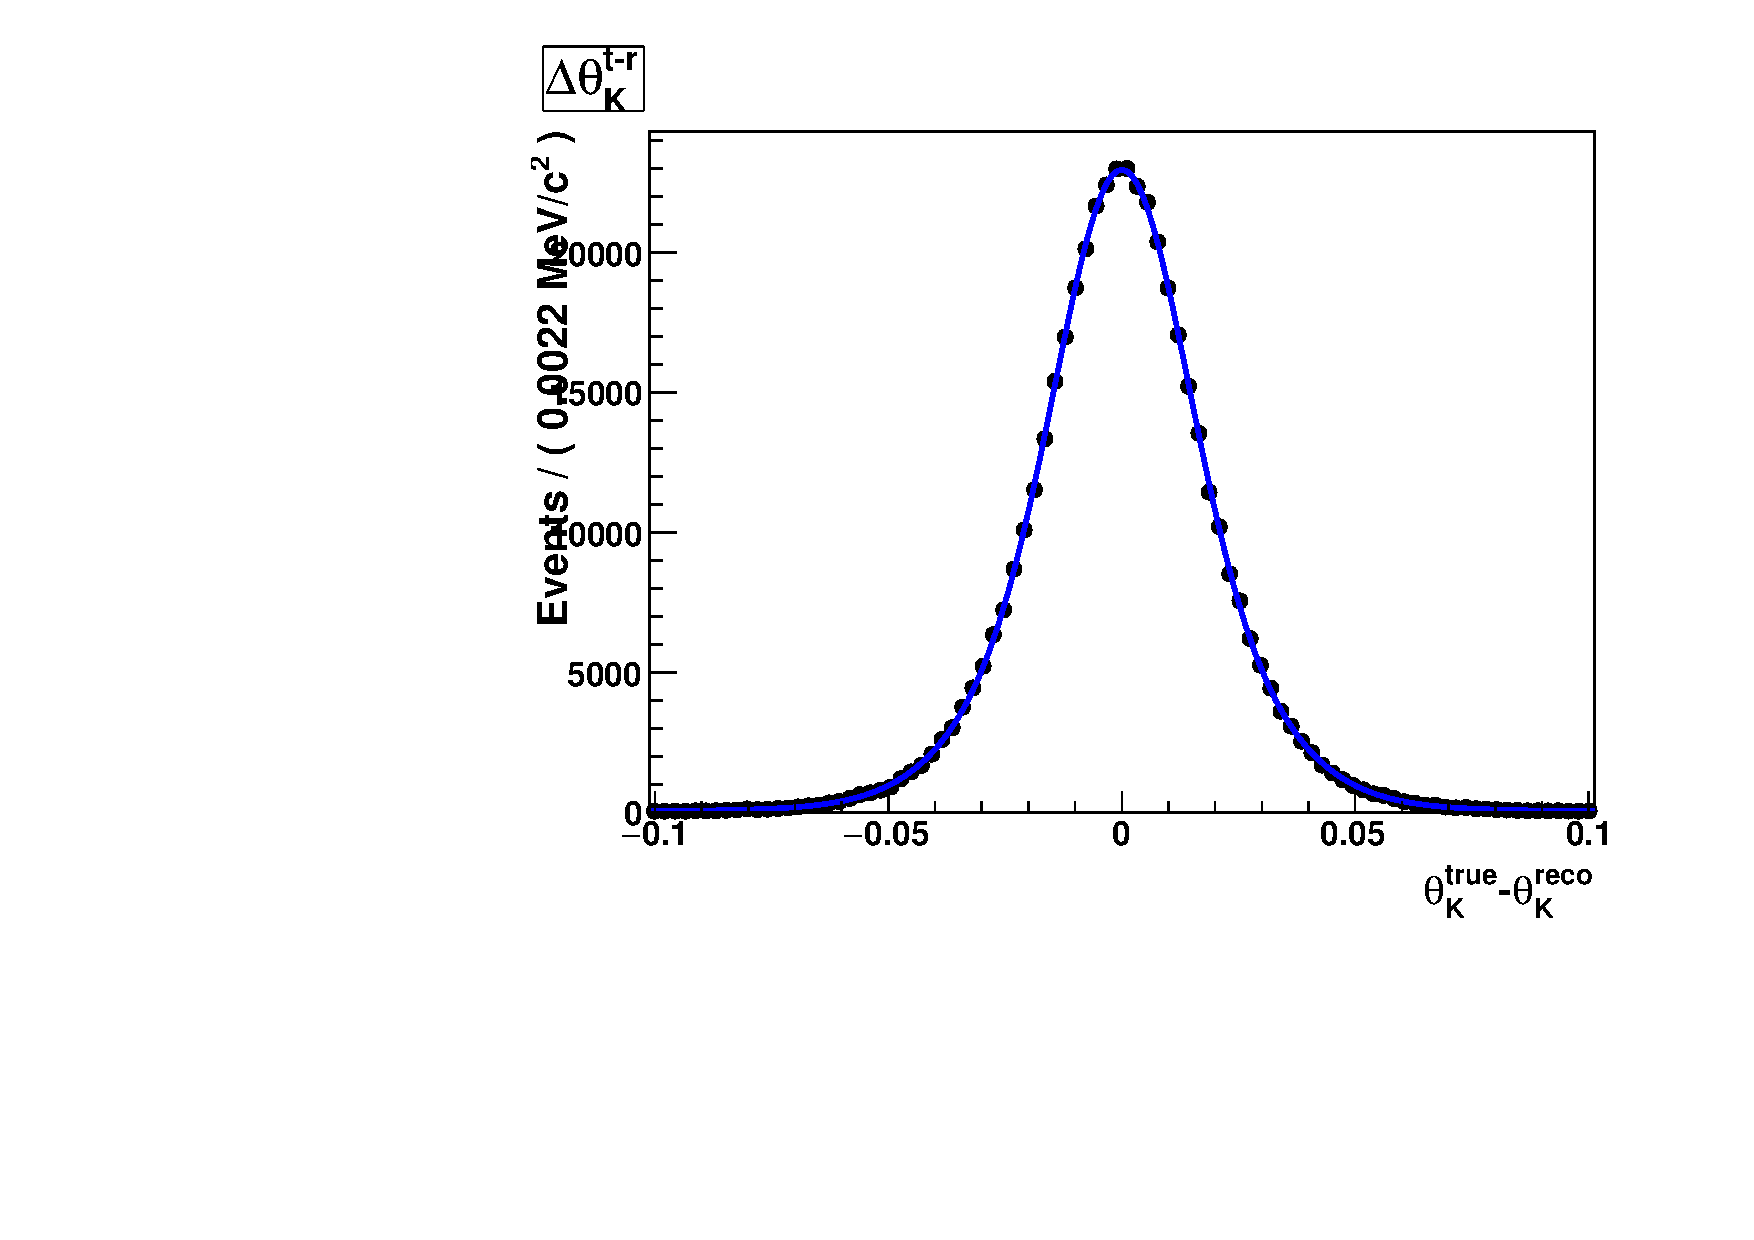
\includegraphics[width=0.47\linewidth]{AnglesRes/MC/thetaK_diff.pdf}
    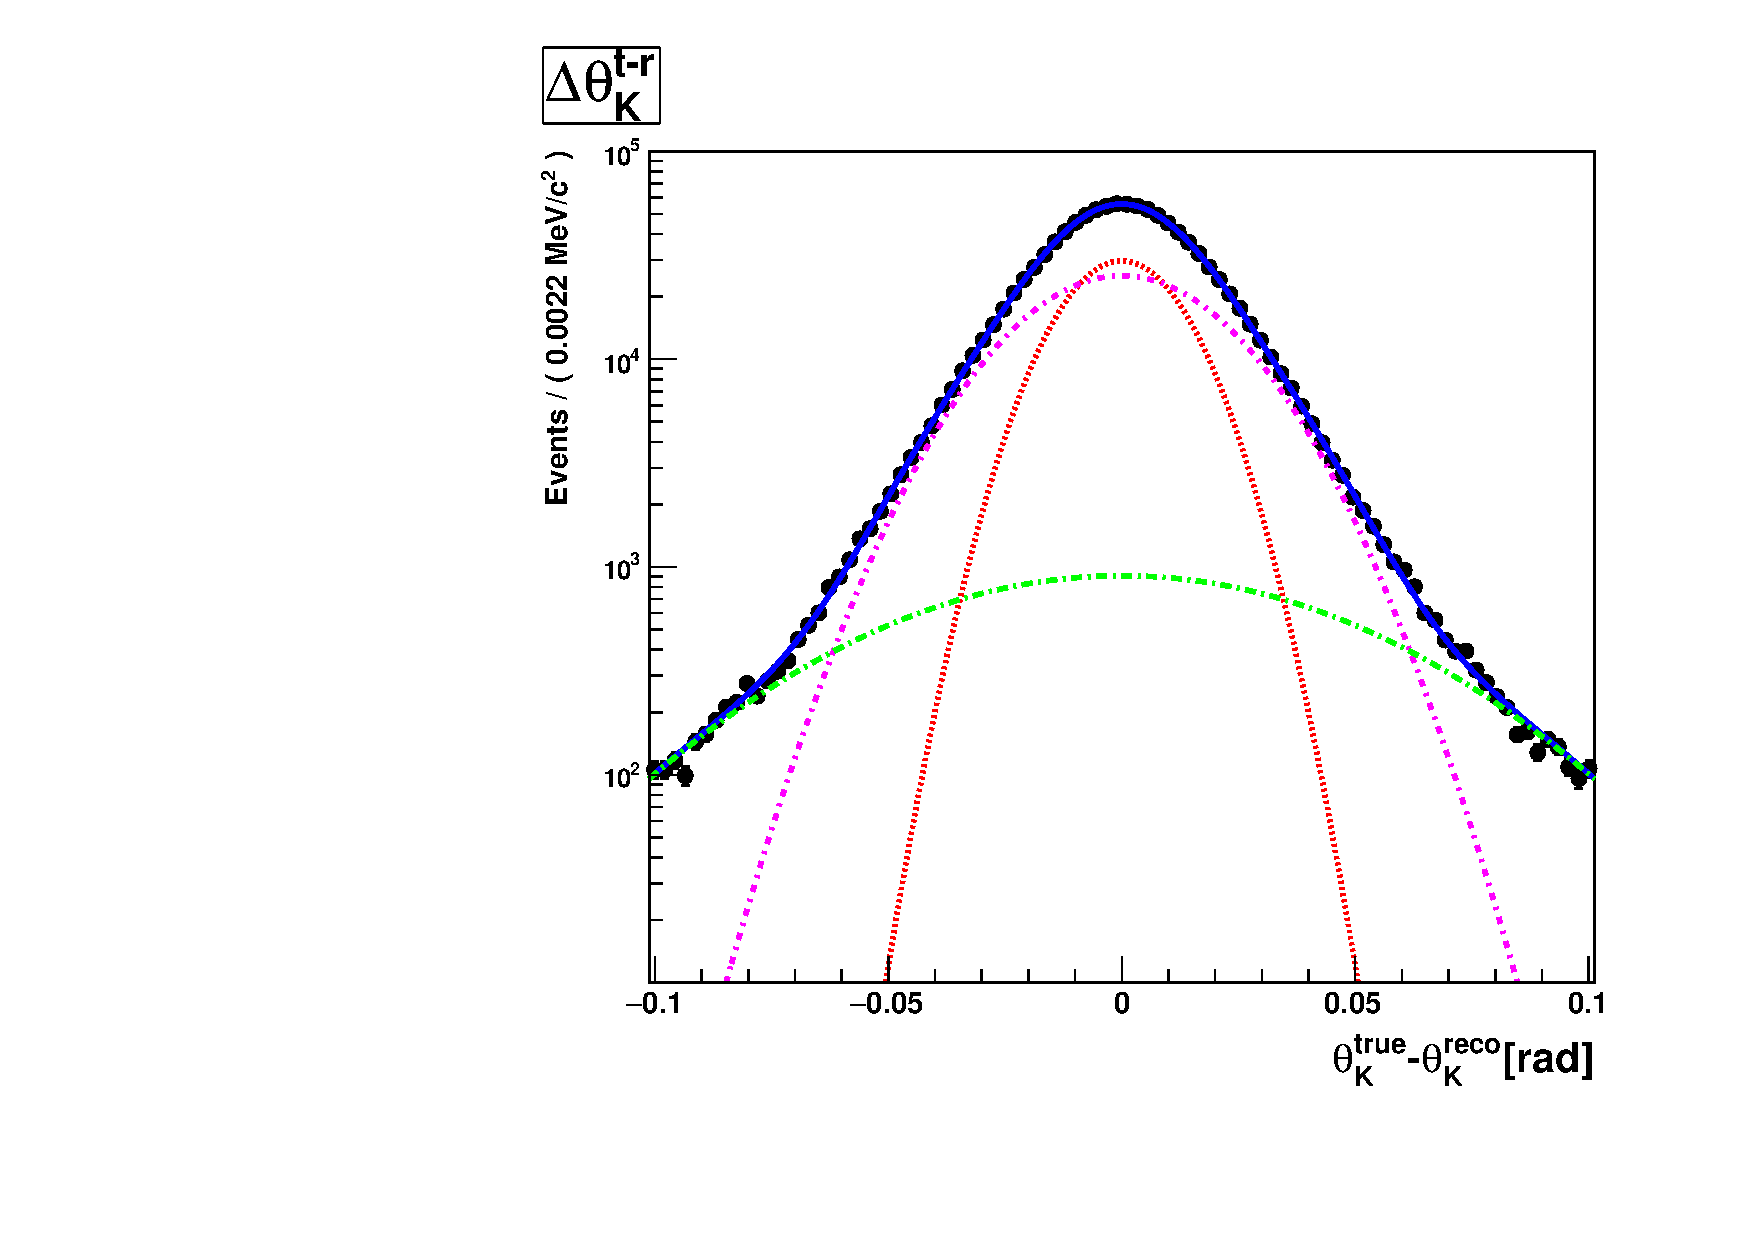
\includegraphics[width=0.47\linewidth]{AnglesRes/MC/thetaK_diff_log_new.pdf}
     \vspace*{-0.5cm}
  \end{center}
  \begin{center}
    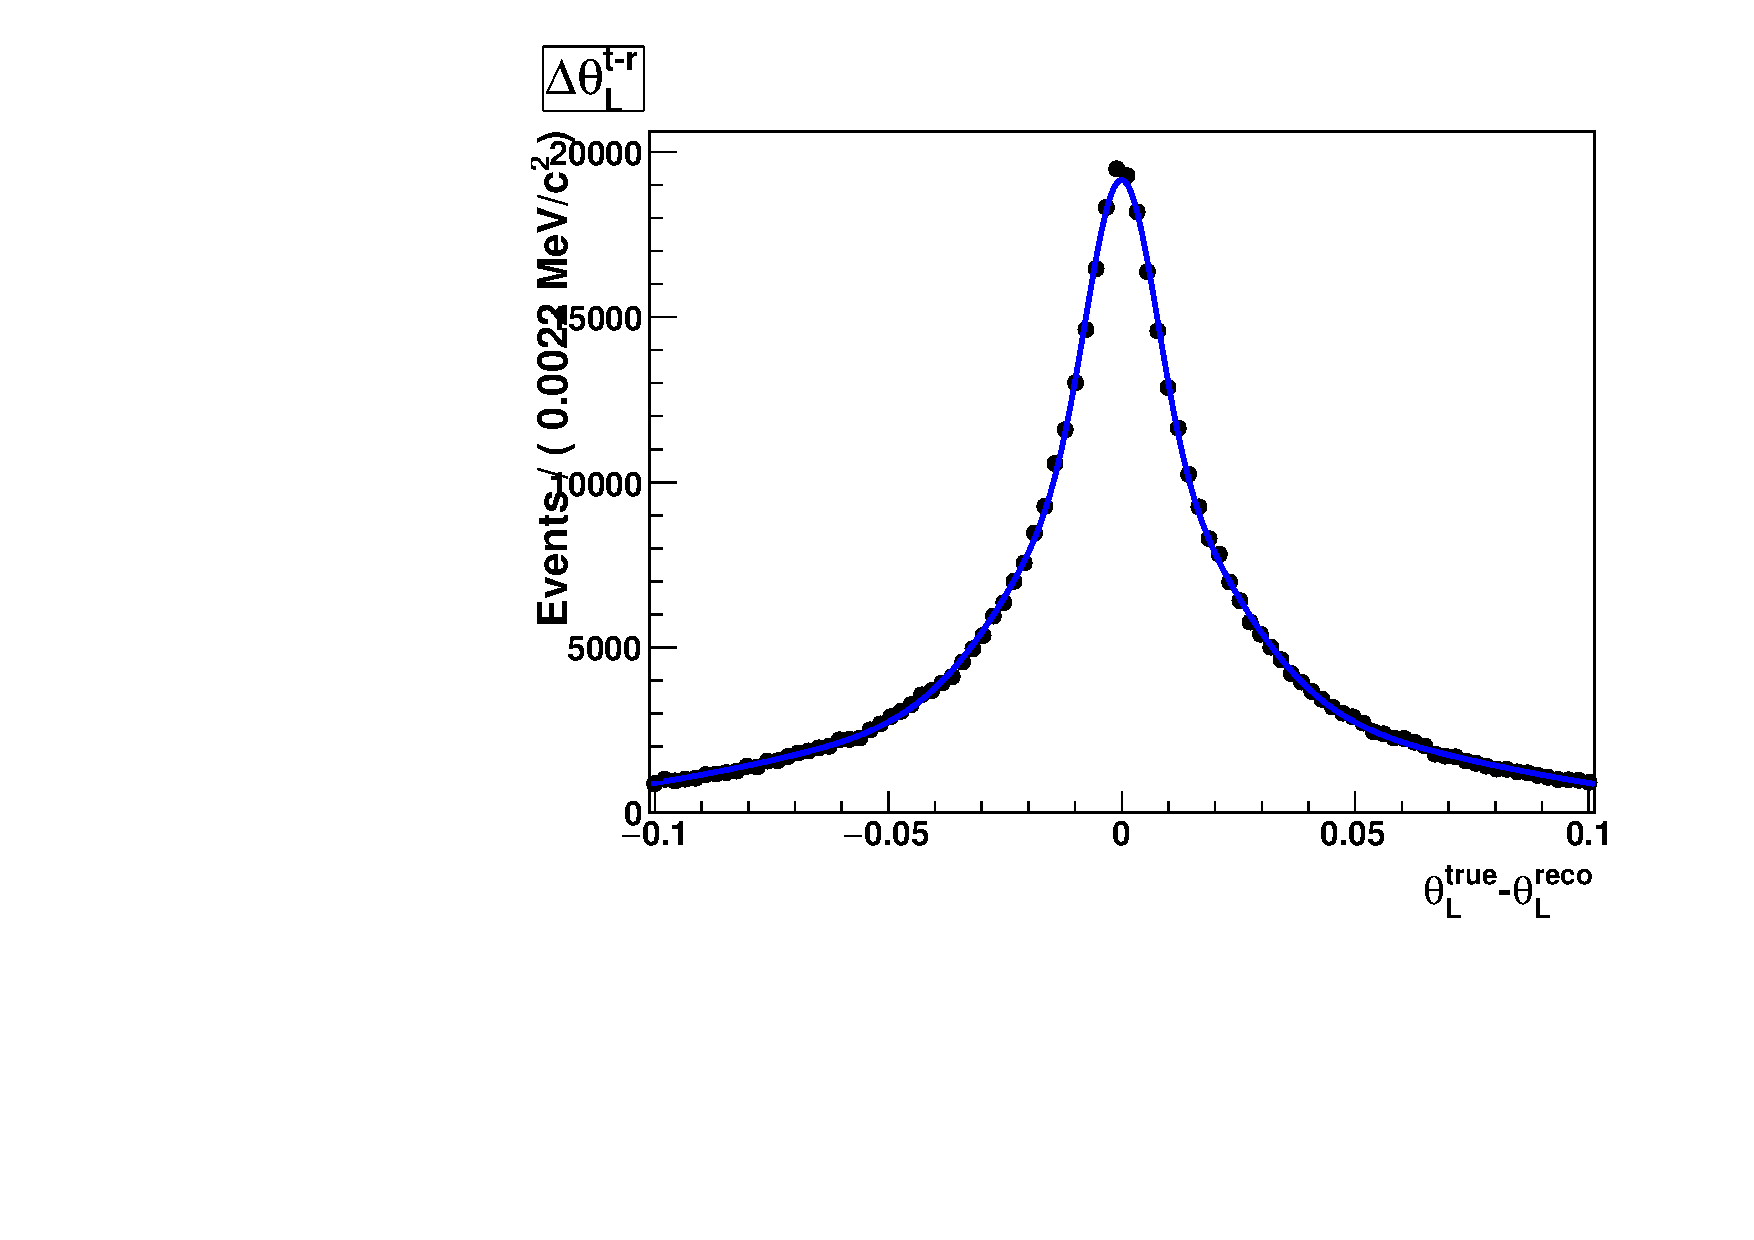
\includegraphics[width=0.47\linewidth]{AnglesRes/MC/thetaL_diff.pdf}
    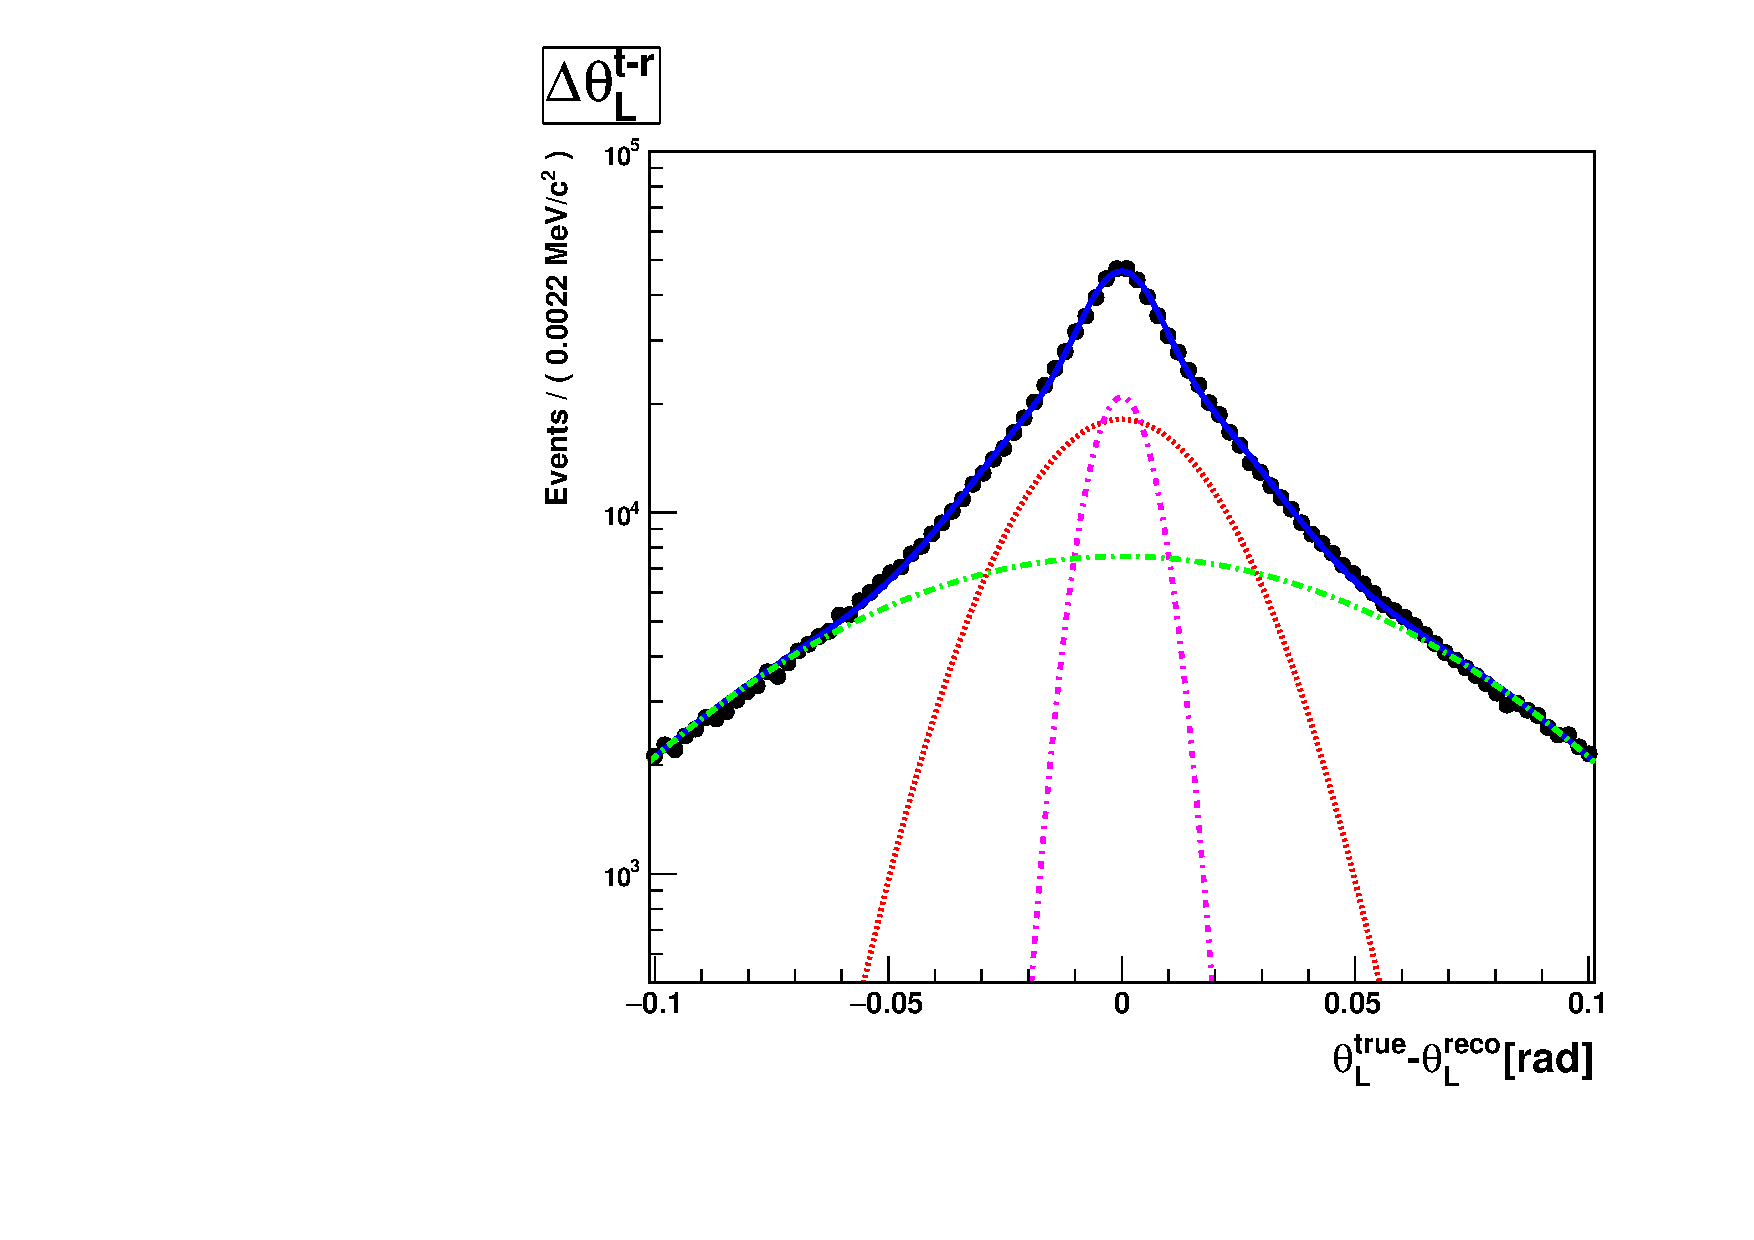
\includegraphics[width=0.47\linewidth]{AnglesRes/MC/thetaL_diff_log_new.pdf}
     \vspace*{-0.5cm}
  \end{center}
  \begin{center}
    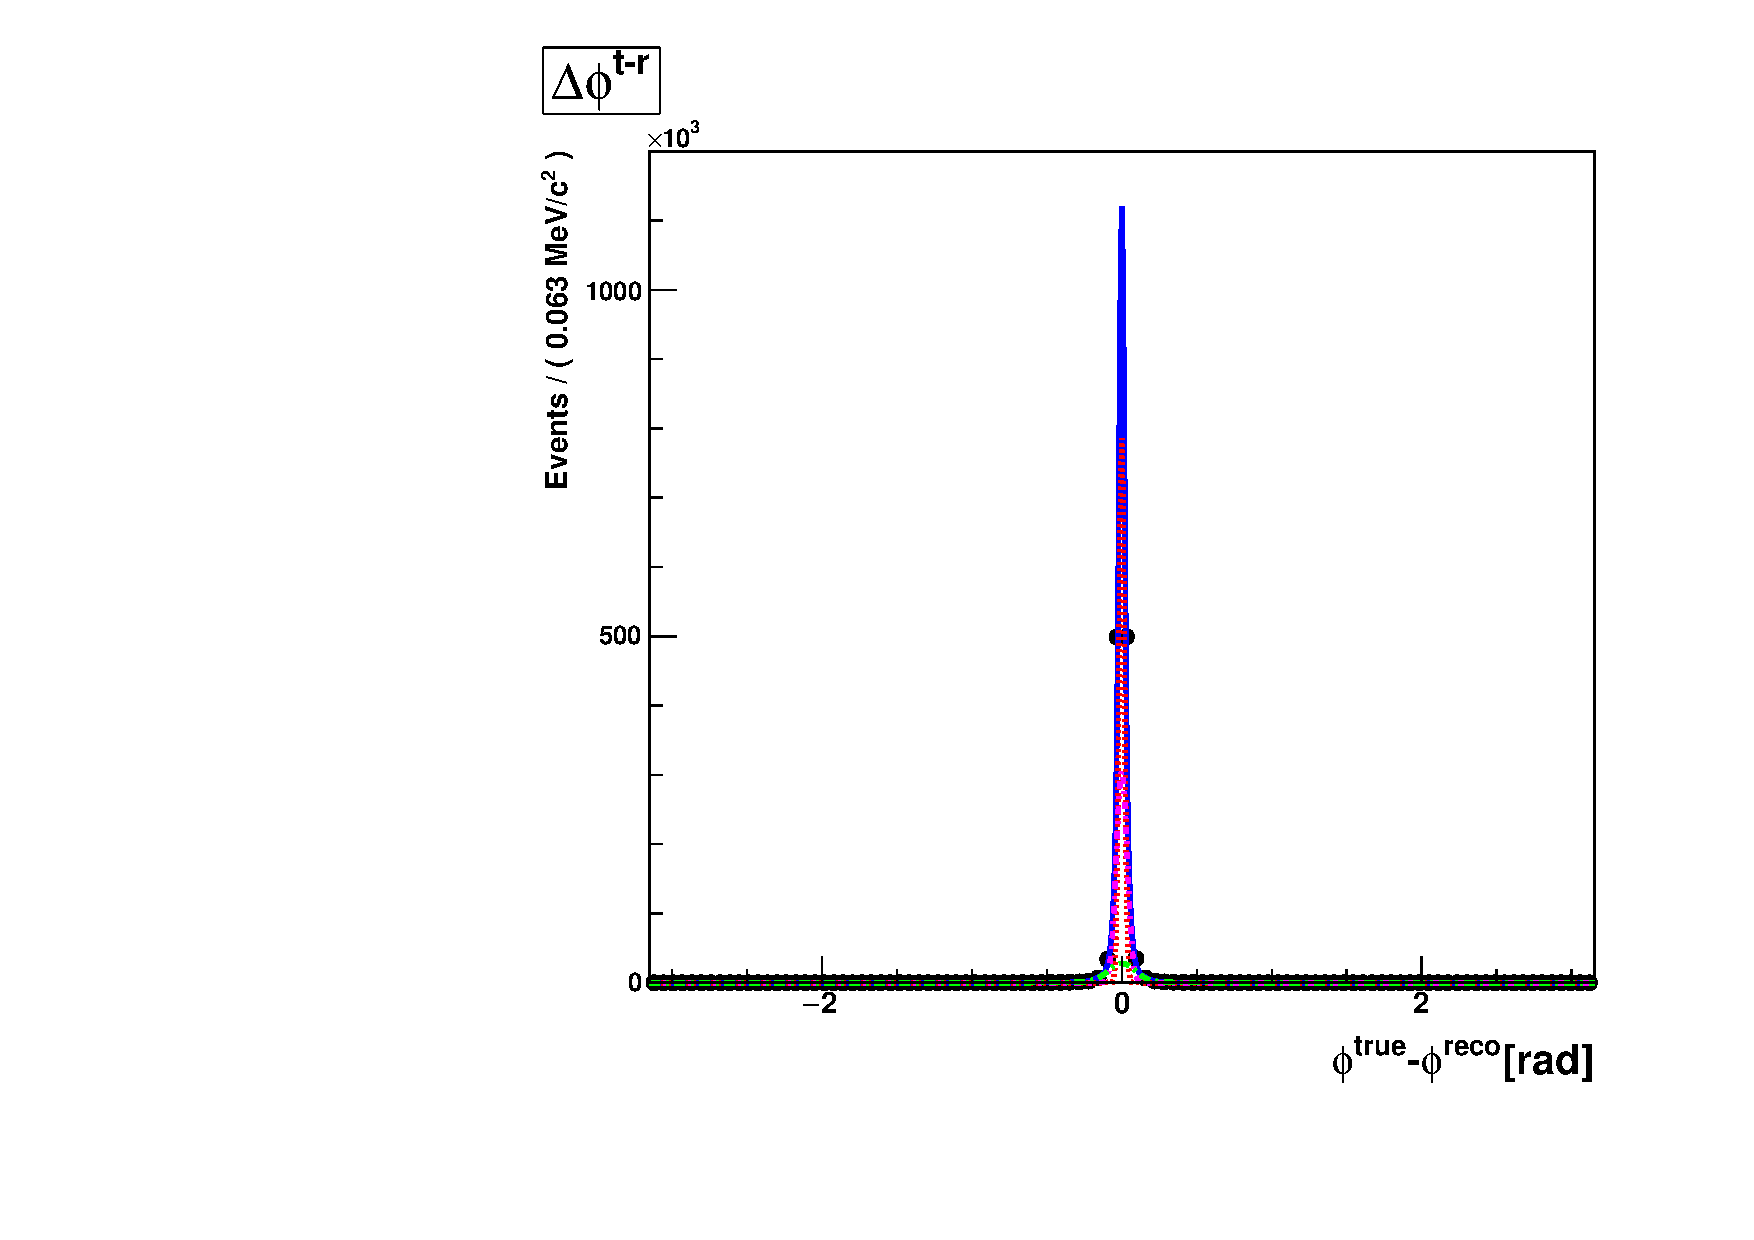
\includegraphics[width=0.47\linewidth]{AnglesRes/MC/phi_diff.pdf}
    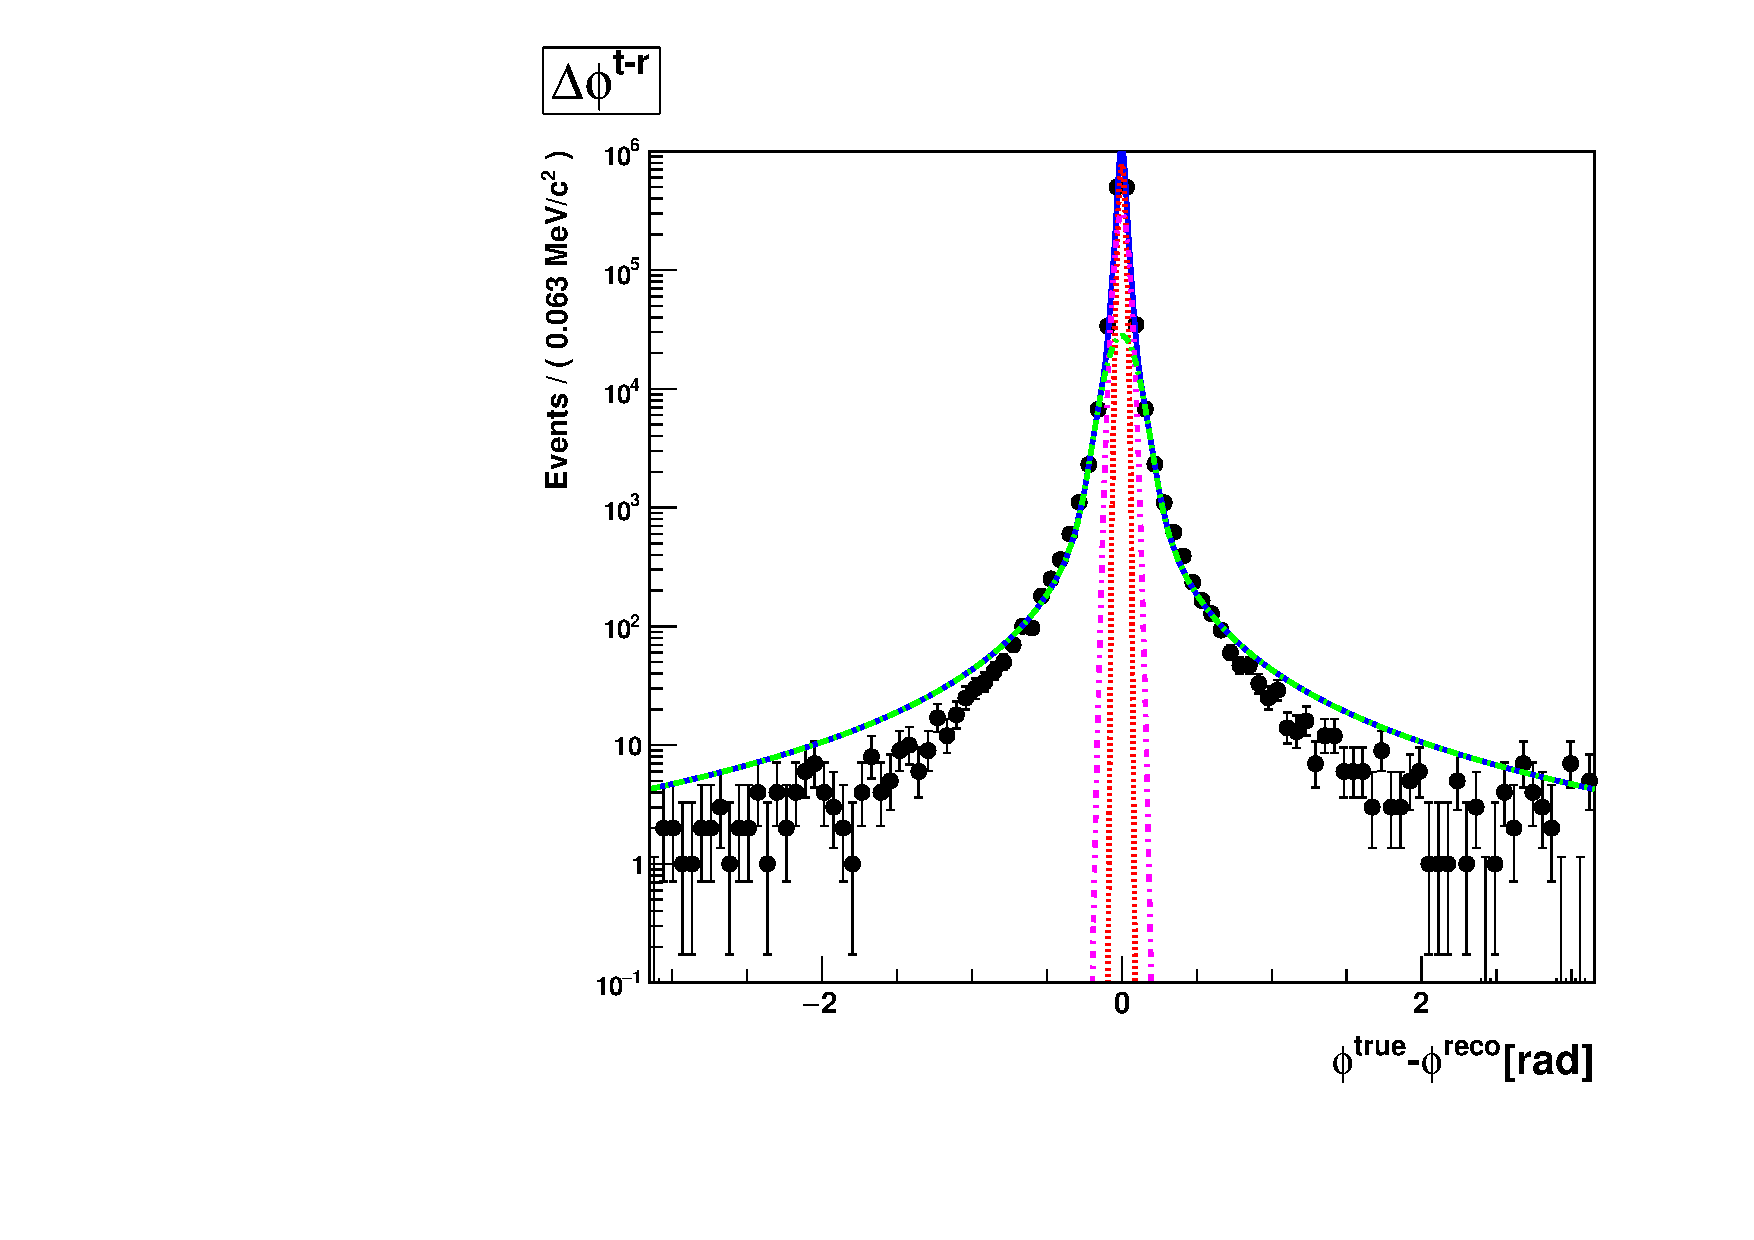
\includegraphics[width=0.47\linewidth]{AnglesRes/MC/phi_diff_log_new.pdf}
    \vspace*{-0.5cm}
  \end{center}
    \caption{
   The distributions of the difference between the true and reconstructed angle from the simulated sample of $\Bs\to\jpsi(\epem)\phi$ decays. A fit is superimposed in each distribution. The right hand side shows the logarithmic scale plots.
}
  \label{fig:AnglesRes} 
\end{figure}
\clearpage

\begin{figure}[hbt]
  \begin{center}
    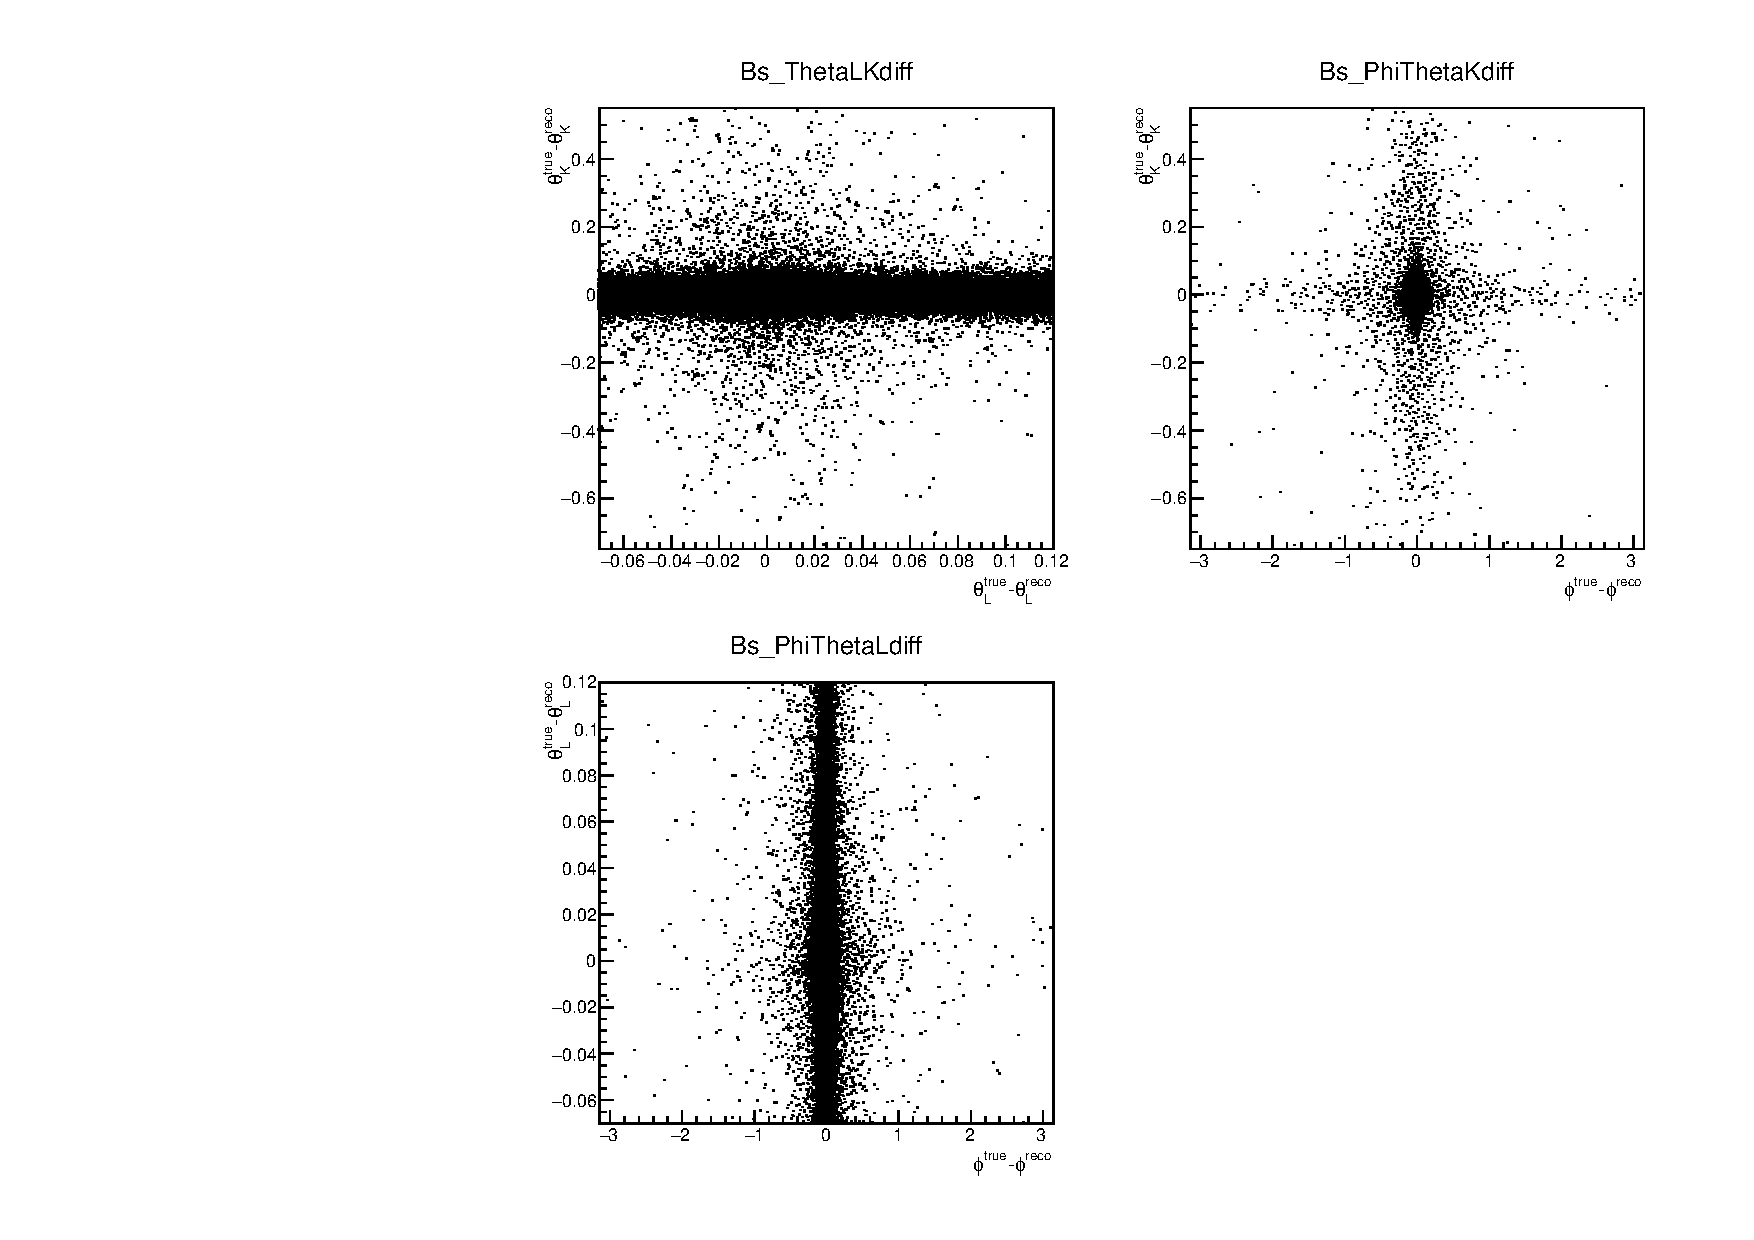
\includegraphics[width=0.9\linewidth]{AnglesRes/MC/AngRes_2D.pdf}
     \vspace*{-0.5cm}
  \end{center}
    \caption{
   The two-dimensional distributions of the helicity angle resolutions obtained from simulated data. The units are in radians in all cases.
}
  \label{fig:AnglesRes2D} 
\end{figure}
\clearpage

\section{Flavour tagging}\label{sec:FlavTagg}

The flavour of the $\Bs$ candidate at production state is inferred by two independent classes of flavour tagging algorithms, the opposite-side (OS) tagger and the same-side kaon (SSK) tagger, which exploit specific features of the incoherent production of $\bquark\bquarkbar$ quark pairs in $pp$ collisions. Each tagging algorithm gives a tag decision and a mistag probability. The tag decision takes three values: +1, -1, or 0, correspond to $\Bs$, $\Bsb$, or untagged $\Bs$ meson, respectively. The fraction of events in the sample with a non-zero tagging decision gives the efficiency of the tagger, $\varepsilon$. The mistag probability, $\eta$, is estimated event-by-event, and it represents the probability that the algorithm assigns a wrong tag decision to the event. It is calibrated using data samples of several flavour specific $\Bz$ and $\Bp$ decays, to obtain the corrected mistag probability, $\mistag$. The corrected mistag probability determines the square dilution factor of the tagger, $\langle\mathcal{D}^{2}\rangle=\langle(1-2\mistag)^{2}\rangle$. The $\langle\mathcal{D}^{2}\rangle$ rescales the efficiency of the tagger to quantify the fraction of the sample equivalent to perfectly tagged events. The effective efficiency, called tagging power, is given by the product of the efficiency and the square dilution factor, $\varepsilon\langle\mathcal{D}^{2}\rangle$.

By means of flavour conservation of the strong interaction, the OS tagger consists of a few algorithms~\cite{Aaij:2012mu}. They infer the signal production flavour from the decay products of the $\bquark$-hadron produced by the other $\bquark$ quark in the event, by using the charge of muons or electrons from second $\Bs$ in semileptonic decays, the net charge of the opposite-side displaced vertex, and the charge of the kaon from opposite-side $\bquark\to\cquark\to\squark$ transitions. All algorithms are combined to provide a single OS tagging response. The cut-based selection of the tagging candidates and the neural networks that calculate the mistag probabilities are optimized for the analysis of the full 2011 and 2012 datasets by using a data sample of $\Bp\to\jpsi\Kp$ decays. As an result, the OS algorithm has tagging power of (3.42$\pm$0.08)$\%$ in $\Bs\to\jpsi(\epem)\phi$ data, with a tagging efficiency of (36.31$\pm$0.45)$\%$. 

The SSK algorithm deduces the signal production flavour by exploiting charge-flavour correlations of the kaon produced during its fragmentation. A selection for the identification of the tagging kaon candidate is based on a neural network (NNetSSK)~\cite{LHCb:2012zja}. The NNetSSK algorithm~\cite{Aaij:2016psi} has a tagging efficiency of (62.83$\pm$0.45)$\%$ and a tagging power of (2.02$\pm$0.05)$\%$ in $\Bs\to\jpsi(\epem)\phi$ data.

The mistag probabilities, $\eta^{\text{alg}}$ (alg = OS, SSK), are calibrated on data to get the corrected probabilities $\mistag^{\text{alg}}$ and $\bar{\mistag}^{\text{alg}}$, for $\Bs$ and $\Bsb$, respectively:
\[
  \mistag^{\text{alg}}=\left(p_{0}^{\text{alg}}+\frac{\Delta p_{0}^{\text{alg}}}{2}\right)+\left(p_{1}^{\text{alg}}+\frac{\Delta p_{1}^{\text{alg}}}{2}\right)(\eta^{\text{alg}}-\langle\eta^{\text{alg}}\rangle)\quad\text{for an initial $\Bs$ event}, 
\]
\begin{equation}\label{eq:mistag}
 \bar{\mistag}^{\text{alg}}=\left(p_{0}^{\text{alg}}-\frac{\Delta p_{0}^{\text{alg}}}{2}\right)+\left(p_{1}^{\text{alg}}-\frac{\Delta p_{1}^{\text{alg}}}{2}\right)(\eta^{\text{alg}}-\langle\eta^{\text{alg}}\rangle)\quad\text{for an initial $\Bsb$ event},
\end{equation}
where $p^{\text{alg}}_{i}$ ($i$ = 0, 1) are the calibration parameters, averaged for $\Bs$ and $\Bsb$ events; $\Delta p^{\text{alg}}_{i}$, called mistag asymmetries, are the difference between the calibration parameters as measured for $\Bs$ and $\Bsb$. The $\langle\eta^{\text{ang}}\rangle$ is the average of the mistag distribution of the $\Bs\to\jpsi(\epem)\phi$ data, unfolded from background with the sPlot technique~\cite{Pivk:2004ty} by using the $\jpsi\phi$ mass as discriminating variable (Fig.~\ref{fig:Mistag}). The parameters used in Eq.~\ref{eq:mistag} are reported in Table~\ref{tab:CalibrationFT}. 
\begin{figure}[hbt]
  \begin{center}
    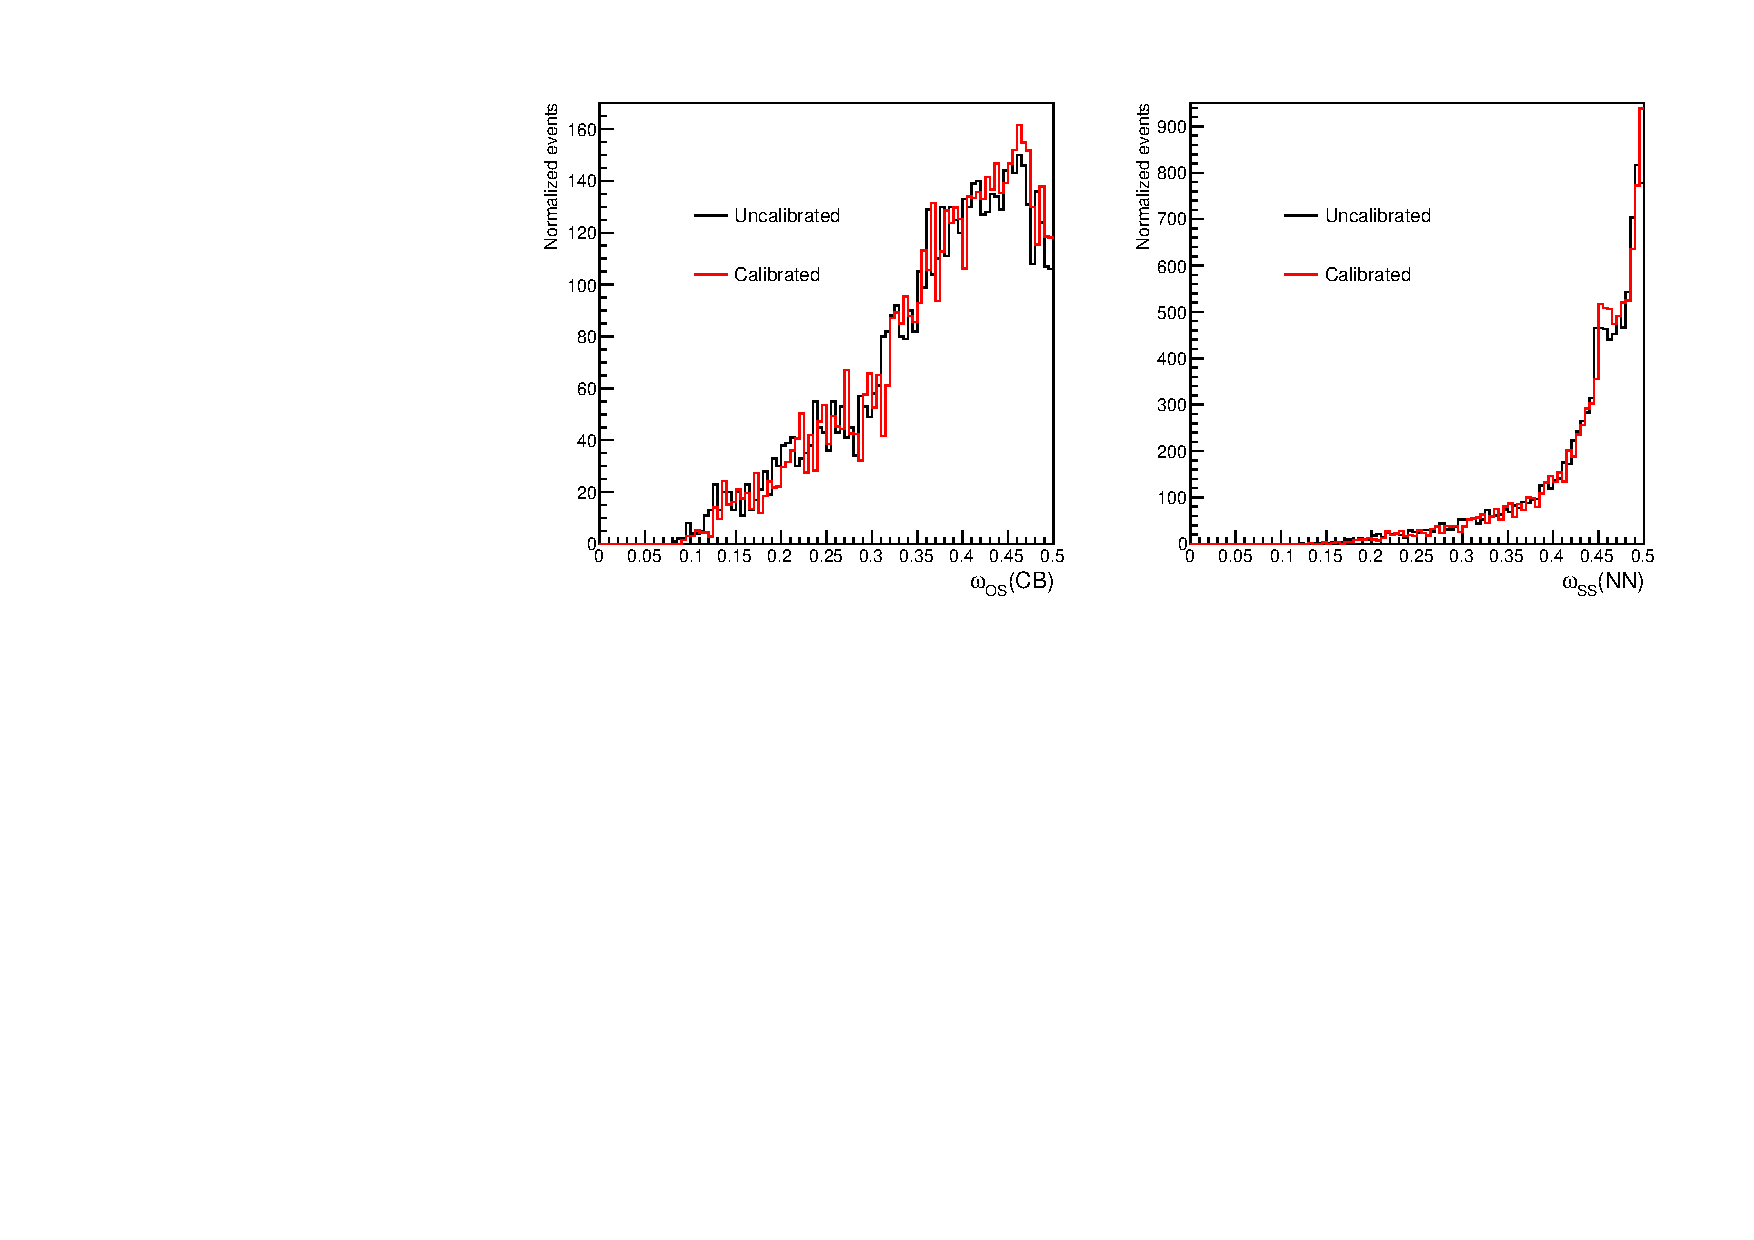
\includegraphics[width=1\linewidth]{Tagging/omega_OS_SS_fullRun1_horizontal.pdf}
     \vspace*{-0.5cm}
  \end{center}
    \caption{
   The OS (left) and SSK (right) mistag distributions for $\Bs\to\jpsi(\epem)\phi$ signal events before (black) and after (red) the calibration.}
  \label{fig:Mistag} 
\end{figure}
They are the results of the standard calibration provided by the Flavour Tagging group~\cite{LHCb:FTa, LHCb:FTb}: $p^{\text{OS}}_{i}$ are the combinations of calibration in data samples of several decays ($\Bu\to\jpsi\Kp$, $\Bu\to\Dz\pip$, $\Bz\to\jpsi\Kstarz$, $\Bz\to\Dstarm\mup X$ and $\Bs\to\Dsm\pip$); the OS mistag asymmetries are measured with $\Bu\to\jpsi\Kp$, $\Bu\to\Dz\pip$ and $\Bz\to\jpsi\Kstarz$ decays; $p^{\text{SSK}}_{i}$ are extracted by measuring the $\Bs$ flavour oscillations in a sample of $\Bs\to\Dsm\pip$ decays; the SSK mistag asymmetries are determined from a sample of prompt $\Dsp\to\phi\pip$ decays, reweighted to match the $\Bs$ kinematic distributions. Systematic uncertainties of calibration parameters address the portability of the calibrations from the control samples to $\Bs\to\jpsi(\epem)\phi$ data; they are dominated by the effect of the different kinematic distributions between the decay modes used in calibration and the $\Bs\to\jpsi(\epem)\phi$ signal data. Such systematic errors are independent from the flavour decision, and they mainly cancel when computing the mistag asymmetries. Their small contribution - approximately 10$\%$ (20$\%$) of the systematic error of $p_{0}$ ($p_{1}$) for $\Delta p_{0}/2$ ($\Delta p_{1}/2$) - are directly included in the single errors of the mistag asymmetries reported in Table~\ref{tab:CalibrationFT}.

 \begin{table}[htb]
  \caption{
   The parameters used in Eq.~\ref{eq:mistag} to calibrate the per-event mistag probabilities. When two uncertainties are quoted, the first one is statistical and the second one is systematic.}
    \small{
\begin{center}\begin{tabular}{ccc}
    Parameter                         &  OS  & SSK  \\ 
    \hline
   $\langle\eta\rangle$& 0.3751&   0.4373 \\
    $p_{0}-\langle\eta\rangle$ &   0.0062$\pm$0.0019$\pm$0.0040 & 0.005$\pm$0.004$\pm$0.003 \\
    $\Delta p_{0}/2$& 0.0070$\pm$0.0006 &    -0.0079$\pm$0.0007 \\
    $p_{1}$ &   0.982$\pm$0.007$\pm$0.034 & 0.976$\pm$0.071$\pm$0.057 \\
    $\Delta p_{1}/2$& 0.033$\pm$0.006 &    0.0035$\pm$0.0111 \\
    \hline
  \end{tabular}\end{center}
  }
\label{tab:CalibrationFT}
\end{table}

The $\Bs\to\jpsi(\epem)\phi$ data sample is split in four independent subsamples, according to the tag decisions: exclusive OS tagged events ($q^{\text{OS}}\neq$0 and $q^{\text{SSK}}$=0), referred to as "OS-only" events; exclusive SSK tagged events ($q^{\text{OS}}$=0 and $q^{\text{SSK}}\neq$0), referred to as "SSK-only" events; OS and SSK tagged events ($q^{\text{OS}}\neq$0 and $q^{\text{SSK}}\neq$0), referred to as "OS$\&$SSK" events; and finally, untagged events ($q^{\text{OS}}$=$q^{\text{SSK}}$=0), which are about 22$\%$ and 26$\%$ of the data and simulation samples, respectively. The fractions, the efficiencies, and the tagging powers of the tagged categories OS-only, SSK-only and OS$\&$SSK as measured for $\Bs\to\jpsi(\epem)\phi$ signal candidates from full 2011 and 2012 datasets and from full simulation sample are reported in Tables~\ref{tab:FTperformanceRDfull} and~\ref{tab:FTperformanceMCfull}, respectively. The total tagging efficiency and tagging power of data sample are (75.70$\pm$0.68)$\%$ and (5.20$\pm$0.10)$\%$, respectively. In case of simulated data, the total tagging efficiency and tagging power are (74.73$\pm$0.13)$\%$ and (5.38$\pm$0.02)$\%$, respectively. The flavour tagging performance obtained using simulation is in agreement with flavour tagging performance for data within statistical uncertainty.

\begin{table}[htb]
  \caption{
   The summary of the tagging efficiency ($\varepsilon$), square dilution factor ($\mathcal{D}^{2}$) and tagging power ($\varepsilon\mathcal{D}^{2}$) for the different categories of tagger, obtained from $\Bs\to\jpsi(\epem)\phi$ {\bf signal candidates from full 2011 and 2012 data samples} after the tagging calibration. The column "Fraction" reports the fraction of events in each category out of the all tagged events. }
    \small{
\begin{center}\begin{tabular}{ccccc}
   \hline
    Category & Fraction($\%$)&$\varepsilon(\%)$ & $\mathcal{D}^{2}$ & $\varepsilon\mathcal{D}^{2}(\%)$\\
  \hline
    OS-only& 17.0 &12.87$\pm$0.31 &  0.0977$\pm$0.0025  &1.26$\pm$0.05 \\
     SSK-only& 52.0 &39.39$\pm$0.46 & 0.0315$\pm$0.0013 & 1.24$\pm$0.04 \\
     OS$\&$SSK& 31.0 &23.44$\pm$0.40 &  0.1152$\pm$0.0020  &2.70$\pm$0.08 \\
    \hline
     Total& 100 &75.70$\pm$0.68 & 0.0687$\pm$0.0033 & 5.20$\pm$0.10 \\
    \hline
    \end{tabular}\end{center}
  }
\label{tab:FTperformanceRDfull}
\end{table}
\begin{table}[htb]
  \caption{
   The summary of the tagging efficiency ($\varepsilon$), square dilution factor ($\mathcal{D}^{2}$) and tagging power ($\varepsilon\mathcal{D}^{2}$) for the different ctegories of tagger, obtained from $\Bs\to\jpsi(\epem)\phi$ {\bf signal candidates from full simulated data sample} after the tagging calibration has been applied. The column "Fraction" reports the fraction of events in each category out of the all tagged events. }
    \small{
\begin{center}\begin{tabular}{ccccc}
   \hline
    Category & Fraction($\%$)&$\varepsilon(\%)$ & $\mathcal{D}^{2}$ & $\varepsilon\mathcal{D}^{2}(\%)$\\
  \hline
    OS-only& 16.7 &12.46$\pm$0.06 &  0.0995$\pm$0.0006 &  1.24$\pm$0.01 \\
     SSK-only& 54.0&40.33$\pm$0.09 &  0.0347$\pm$0.0003 &  1.40$\pm$0.01 \\
     OS$\&$SSK& 29.3&21.94$\pm$0.07 &  0.1249$\pm$0.0005 &  2.74$\pm$0.02 \\
    \hline
     Total& 100 &74.73$\pm$0.13 & 0.0720$\pm$0.0008 & 5.38$\pm$0.02 \\
    \hline
    \end{tabular}\end{center}
  }
\label{tab:FTperformanceMCfull}
\end{table}

The time dependent angular decay rate without taking into account any resolution and acceptance effect, $R(t, \Omega|q^{\text{alg}}, \eta^{\text{alg}})$, can be written as:
\[
 R(t, \Omega|q^{\text{alg}}, \eta^{\text{alg}})=(1+q^{\text{OS}}(1-2\omega^{\text{OS}}))(1+q^{\text{SSK}}(1-2\omega^{\text{SSK}}))R(t,\Omega|\Bs)
\]
\begin{equation}\label{eq:decayrate_time_FT}
   +(1-q^{\text{OS}}(1-2\bar{\omega}^{\text{OS}}))(1-q^{\text{SSK}}(1-2\bar{\omega}^{\text{SSK}}))R(t,\Omega|\Bsb),
\end{equation}
where $R(t,\Omega|\Bs)$ and $R(t,\Omega|\Bsb)$ are the time dependent angular decay rates for an initial $\Bs$ and $\Bsb$, respectively; $\omega$ and $\bar{\omega}$ are derived from Eq.~\ref{eq:mistag}. By considering $q^{\text{OS}}$=0 and $q^{\text{SSK}}$=0 as a special tagging decision, Eq.~\ref{eq:decayrate_time_FT} provides a unified form of the time dependent angular decay rate for any of the four independent categories considered, i.e. no matter a tagging decision is (or both decisions are) zero. 

\subsection{OS calibration on $\Bp\to\jpsi(\mumu)\Kp$ and $\Bp\to\jpsi(\epem)\Kp$ decays}

Since the final state of $\Bs\to\jpsi\phi$ decay includes $\epem$ particles the OS calibrations on $\Bp\to\jpsi(\mumu)\Kp$ and $\Bp\to\jpsi(\epem)\Kp$ are applied. As determined in Sec.~\ref{sec:FlavTagg} the OS algorithm on $\Bp\to\jpsi(\mumu)\Kp$ has tagging power of (3.42$\pm$0.08)$\%$ in $\Bs\to\jpsi(\epem)\phi$ data, with a tagging efficiency of (36.31$\pm$0.45)$\%$. In case electron mode of $\Bp\to\jpsi\Kp$, the OS algorithm has tagging power of (3.20$\pm$0.07)$\%$ and a tagging efficiency of (36.74$\pm$0.45)$\%$ in $\Bs\to\jpsi(\epem)\phi$ data. 

The same SSK algorithm (Sec.~\ref{sec:FlavTagg}) has been applied to both channels.

To get the corrected probabilities $\omega^{OS}$ and $\bar{\omega}^{OS}$, the mistag probability, $\eta^{OS}$, is calibrated on data as defined in Eq.~\ref{eq:mistag}. The mistag distributions of the sWeighted $\Bs\to\jpsi\phi$ data before and after two OS calibrations are shown in Fig.~\ref{fig:MistagOS}. The parameters reported in Table~\ref{tab:CalibrationFTOS} are the results of the calibration provided by the Flavour Tagging group~\cite{LHCb:FTa, LHCb:FTc} for muon and electron modes of $\Bp\to\jpsi\Kp$ decay. 

\begin{figure}[hbt]
  \begin{center}
    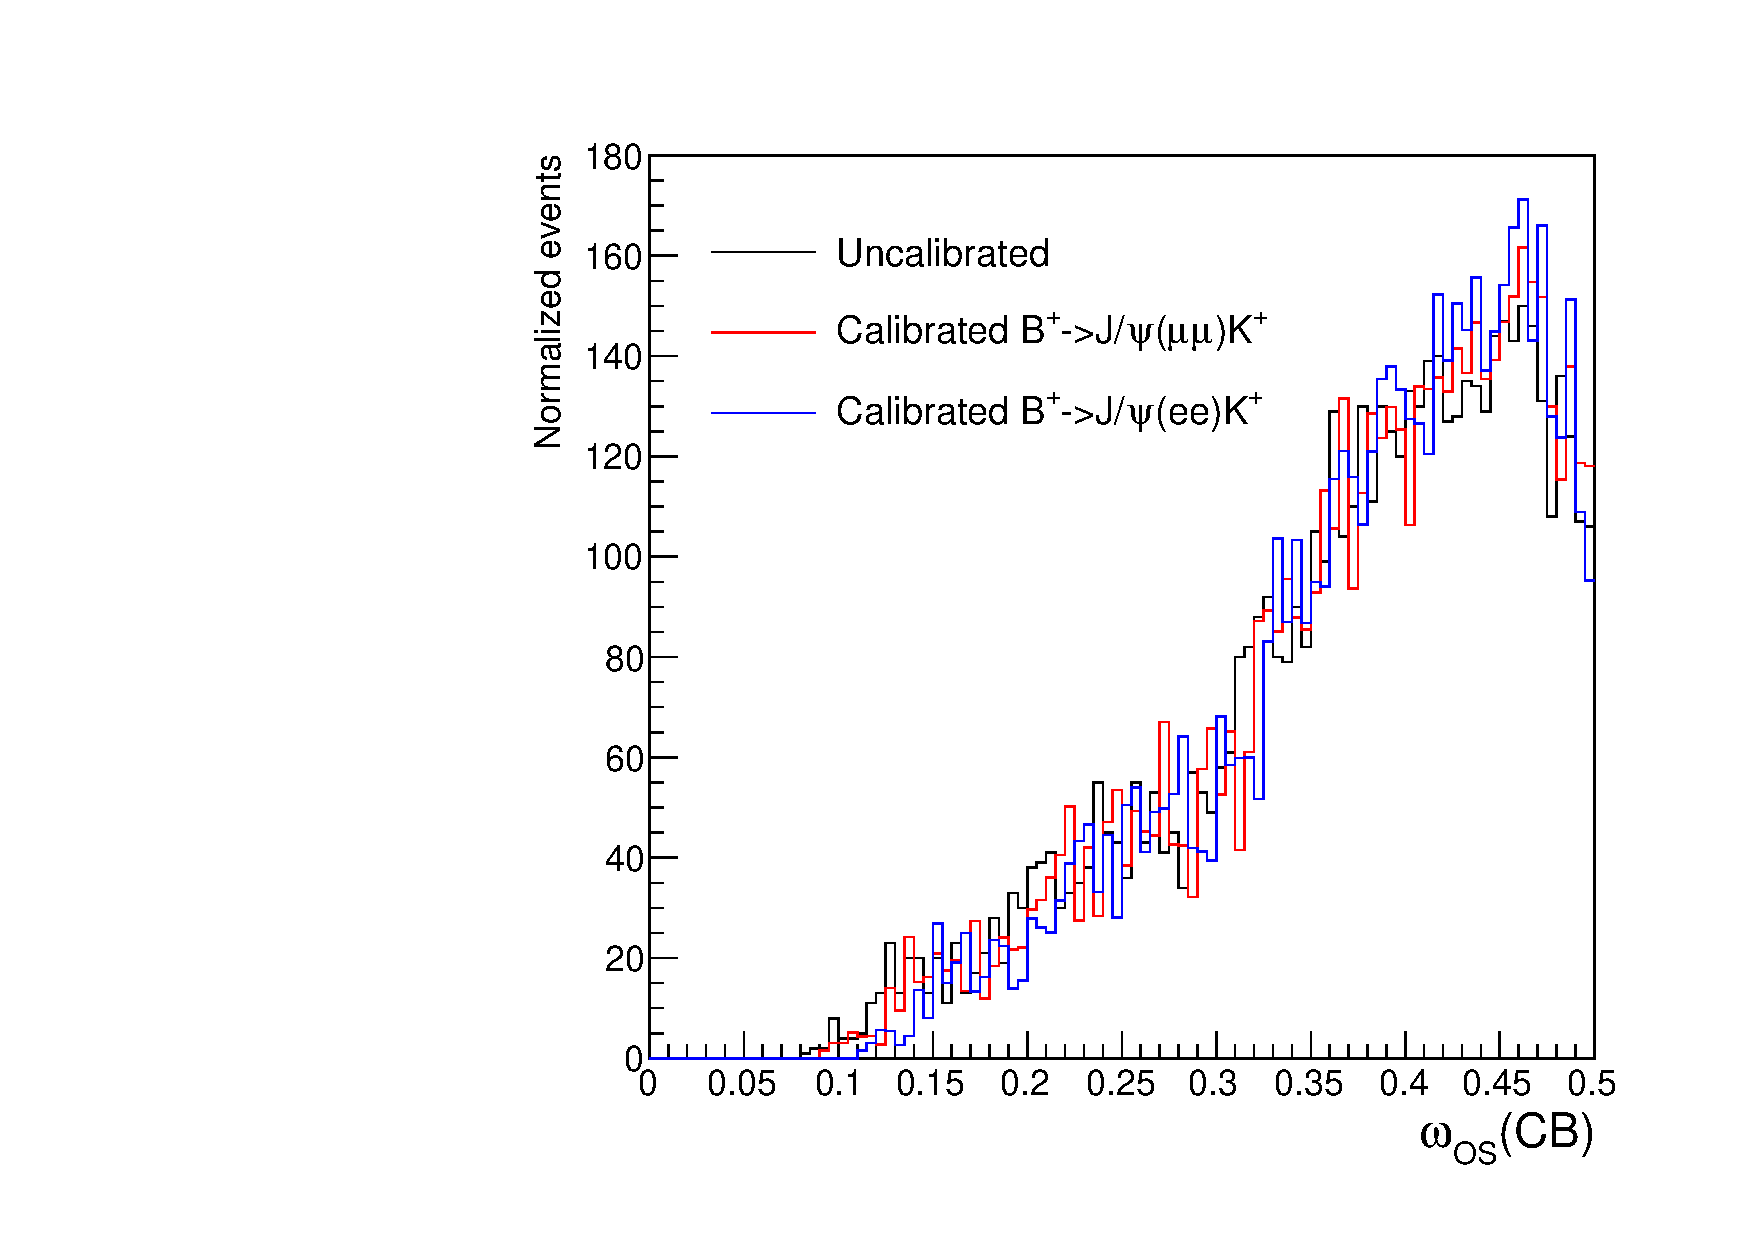
\includegraphics[width=0.6\linewidth]{Tagging/omega_Bu2JpsieeK_Bu2JpsiMuMuK_OS_fullRun1.pdf}
     \vspace*{-0.5cm}
  \end{center}
    \caption{
   The OS mistag distributions for $\Bs\to\jpsi\phi$ signal events before (black) and after the calibration on $\Bp\to\jpsi(\mumu)\Kp$ (red) and $\Bp\to\jpsi(\epem)\Kp$ (blue).}
  \label{fig:MistagOS} 
\end{figure}

 \begin{table}[htb]
  \caption{
   The parameters used in Eq.~\ref{eq:mistag} to calibrate the per-event mistag probabilities for OS calibration. When two uncertainties are quoted, the first one is statistical and the second one is systematic.}
    \small{
\begin{center}\begin{tabular}{ccc}
    Parameter                         &  $\Bp\to\jpsi(\mumu)\Kp$  & \Bp\to\jpsi(\mumu)\Kp  \\ 
    \hline
    $\langle\eta\rangle$ & 0.3751 &    0.3789 \\
    $p_{0}-\langle\eta\rangle$ &   0.0062$\pm$0.0019$\pm$0.0040 & 0.0086$\pm$0.0021 \\
    $\Delta p_{0}/2$& 0.0070$\pm$0.0006 &    0.0083$\pm$0.0021 \\
    $p_{1}$ &   0.982$\pm$0.007$\pm$0.034 & 0.931$\pm$0.021 \\
    $\Delta p_{1}/2$& 0.033$\pm$0.006 &    0.0115$\pm$0.0205 \\
    \hline
  \end{tabular}\end{center}
  }
\label{tab:CalibrationFTOS}
\end{table}

The $\Bs\to\jpsi(\epem)\phi$ dataset is divided in four independent subsamples as described in Sec.~\ref{sec:FlavTagg}. The fractions, the efficiencies, and the tagging powers calculated for OS calibration on $\Bp\to\jpsi(\mumu)\Kp$ and $\Bp\to\jpsi(\epem)\Kp$ as measured for $\Bs\to\jpsi(\epem)\phi$ signal candidates from full 2011 and 2012 datasets and from full simulation sample are reported in Table~\ref{tab:FTperformanceRDfull},~\ref{tab:FTperformanceRDfullOS} and Table~\ref{tab:FTperformanceMCfull},~\ref{tab:FTperformanceMCfullOS}, respectively. The total tagging efficiency and tagging power of data sample are (75.70$\pm$0.68)$\%$ and (5.20$\pm$0.10)$\%$ with OS calibration on muon mode of $\Bp\to\jpsi\Kp$ and (75.80$\pm$0.68)$\%$ and (4.98$\pm$0.10)$\%$ for OS calibration on $\Bp\to\jpsi\Kp$ with electron final state. In case of simulated data, the total tagging efficiency and tagging power are (74.73$\pm$0.13)$\%$ and (5.38$\pm$0.02)$\%$ with OS calibration on $\Bp\to\jpsi(\mumu)\Kp$ and (74.90$\pm$0.13)$\%$ and (5.17$\pm$0.02)$\%$ with OS calibration on $\Bp\to\jpsi(\epem)\Kp$ decay. The flavour tagging perfromance calculated for OS calibration on electron mode of $\Bp\to\jpsi\Kp$ slightly decreases the tagging performance of $\Bs\to\jpsi(\epem)\phi$ signal events. It is considered as a source of systematic uncertainty in Sec.~\ref{subsec:Syst:FT}. 

\begin{table}[htb]
  \caption{
   The summary of the tagging efficiency ($\varepsilon$), square dilution factor ($\mathcal{D}^{2}$) and tagging power ($\varepsilon\mathcal{D}^{2}$) for the different categories of tagger, obtained from $\Bs\to\jpsi(\epem)\phi$ {\bf signal candidates from full 2011 and 2012 data samples} after the OS tagging calibration on $\Bs\to\jpsi(\epem)\phi$ has been applied. The column "Fraction" reports the fraction of events in each category out of the all tagged events.}
    \small{
\begin{center}\begin{tabular}{ccccc}
   \hline
    Category & Fraction($\%$)&$\varepsilon(\%)$ & $\mathcal{D}^{2}$ & $\varepsilon\mathcal{D}^{2}(\%)$\\
  \hline
    OS-only& 17.1 &12.98$\pm$0.32 &  0.0901$\pm$0.0024 & 1.17$\pm$0.05 \\
     SSK-only& 51.5 &39.06$\pm$0.46 & 0.0315$\pm$0.0013  & 1.23$\pm$0.04 \\
     OS$\&$SSK& 31.4 &23.76$\pm$0.40 &  0.1086$\pm$0.0020 & 2.58$\pm$0.08 \\
    \hline
     Total& 100 &75.80$\pm$0.68 & 0.0657$\pm$0.0033& 4.98$\pm$0.10 \\
    \hline
    \end{tabular}\end{center}
  }
\label{tab:FTperformanceRDfullOS}
\end{table}

\begin{table}[htb]
  \caption{
   The summary of the tagging efficiency ($\varepsilon$), square dilution factor ($\mathcal{D}^{2}$) and tagging power ($\varepsilon\mathcal{D}^{2}$) for the different categories of tagger, obtained from $\Bs\to\jpsi(\epem)\phi$ {\bf signal candidates from full simulated data sample} after the OS tagging calibration on $\Bs\to\jpsi(\epem)\phi$ has been applied. The column "Fraction" reports the fraction of events in each category out of the all tagged events. }
    \small{
\begin{center}\begin{tabular}{ccccc}
   \hline
    Category & Fraction($\%$)&$\varepsilon(\%)$ & $\mathcal{D}^{2}$ & $\varepsilon\mathcal{D}^{2}(\%)$\\
  \hline
    OS-only& 16.9 &12.65$\pm$0.06 &  0.0917$\pm$0.0006 &  1.16$\pm$0.01 \\
     SSK-only& 55.7&40.03$\pm$0.09 &  0.0347$\pm$0.0003 &  1.39$\pm$0.01 \\
     OS$\&$SSK& 27.4&22.22$\pm$0.07 &  0.1179$\pm$0.0005 &  2.62$\pm$0.02 \\
    \hline
     Total& 100 &74.90$\pm$0.13 & 0.0690$\pm$0.0008 & 5.17$\pm$0.02 \\
    \hline
    \end{tabular}\end{center}
  }
\label{tab:FTperformanceMCfullOS}
\end{table}

\clearpage

\section{Results of likelihood fit}\label{sec:Results}

Table~\ref{tab:FitResults} shows the $\Bs\to\jpsi(\epem)\phi$ final results of the fit to 3~$\invfb$ of LHCb dataset including decay time and angular acceptance effect, decay time resolution and fixed flavour tagging calibration. A blind string has been applied in the fit for $\Gs$, $\DGs$ and $\phis$. The correlation matrix of the fit is shown in Table~\ref{tab:CorrelationMatrix}. The projections of the fit result on the decay time and helicity angle distributions are shown in Fig.~\ref{fig:TimeAngleFit} ({\tt Preliminary}).

\begin{table}[htb]
  \caption{
   The results of the unbinned maximum likelihood fit to the selected $\Bs\to\jpsi(\epem)\phi$ candidates including all acceptance and resolution effects. The tagging calibration parameters and $\dms$ are Gaussian constrained in the fit. The values for $\Gs$, $\DGs$ and $\phis$ are blinded. The uncertainty is statistical. {\tt Preliminary}}
    \small{
\begin{center}\begin{tabular}{cc}
Parameter & Fit result and error \\ 		\hline
            $\Gamma_{s}$ [$\ps^{-1}$] &       $X.XXX \pm$ 0.0057                \\
      $\Delta\Gamma_{s}$ [$\ps^{-1}$]&         $X.XXX \pm$  0.0155                \\
$A_{\hspace{-1pt}\perp}^{2}$ &      0.2750 $\pm$   0.0121                \\
             $A_0^2$ &      0.5025 $\pm$  0.0088                \\
  $\delta_\parallel$ [$\rad$] &       3.0092 $\pm$    0.1759                \\
      $\delta_\perp$ [$\rad$] &          3.1086 $\pm$    0.3686                \\
               $F_S$ &     0.0735 $\pm$   0.0167                \\
          $\delta_S$ [$\rad$] &     -0.1093 $\pm$   0.0801                \\
            $\phi_s$ [$\rad$] &      $X.XXX \pm$    0.1548                \\
           $\lambda$ &      0.9836 $\pm$   0.0261                \\
           $\Delta m_s$~[ps$^{-1}$] &       18.176 $\pm$    0.147                \\
\hline
\end{tabular}\end{center}
  }
\label{tab:FitResults}
\end{table}

\begin{sidewaystable}[htb]
  \caption{
   the statistical correlation matrix from nominal fit. {\tt Preliminary}
}
    \small{
\begin{center}\begin{tabular}{@{}|l|r|r|r|r|r|r|r|r|r|r|r|r|r|r|r|@{}}
\hline
& $\Gamma$ & $\Delta\Gamma$ & $A_{\hspace{-1pt}\perp}^{2}$ & $A_0^2$ & $\delta_\parallel$ & $\delta_\perp$ & $F_S$ & $\delta_S$ & $\Delta m_s$ & $\phi_s$ & $\lambda$ & $\omega_{P1}^{OS}$ & $\omega_{P0}^{OS}$ & $\omega_{P1}^{SS}$ & $\omega_{P0}^{SS}$\\ \hline \hline
$\Gamma$ & 1.00 & -0.31 & 0.22 & -0.18 & 0.02 & 0.01 & 0.13 & 0.02 & 0.01 & 0.03 & 0.02 & -0.00 & 0.00 & -0.00 & 0.00 \\
$\Delta\Gamma$ &  & 1.00 & \bf{-0.54} & \bf{0.52} & -0.00 & 0.01 & -0.14 & -0.02 & 0.01 & -0.01 & -0.02 & 0.00 & -0.00 & 0.00 & -0.00 \\
$A_{\hspace{-1pt}\perp}^{2}$ &  &  & 1.00 & \bf{-0.52} & 0.17 & 0.06 & 0.01 & 0.02 & 0.03 & 0.04 & 0.04 & -0.00 & -0.00 & -0.00 & 0.00 \\
$A_0^2$ &  &  &  & 1.00 & 0.02 & -0.01 & -0.00 & 0.00 & -0.01 & -0.03 & 0.00 & 0.00 & 0.00 & 0.00 & -0.00 \\
$\delta_\parallel$ &  &  &  &  & 1.00 & 0.21 & 0.08 & 0.00 & 0.06 & 0.02 & 0.14 & -0.01 & -0.01 & -0.02 & 0.02 \\
$\delta_\perp$ &  &  &  &  &  & 1.00 & 0.01 & -0.02 & \bf{0.79} & 0.39 & 0.19 & -0.02 & -0.01 & 0.01 & 0.02 \\
$F_S$ &  &  &  &  &  &  & 1.00 & 0.17 & 0.06 & 0.06 & 0.14 & -0.02 & 0.04 & -0.02 & 0.02 \\
$\delta_S$ &  &  &  &  &  &  &  & 1.00 & 0.10 & 0.06 & 0.05 & -0.01 & 0.00 & -0.00 & 0.01 \\
$\Delta m_s$ &  &  &  &  &  &  &  &  & 1.00 & 0.47 & 0.17 & -0.02 & -0.01 & 0.02 & 0.02 \\
$\phi_s$ &  &  &  &  &  &  &  &  &  & 1.00 & 0.05 & -0.05 & -0.02 & -0.01 & -0.02 \\
$\lambda$ &  &  &  &  &  &  &  &  &  &  & 1.00 & -0.01 & 0.01 & -0.00 & 0.00 \\
$\omega_{P1}^{OS}$ &  &  &  &  &  &  &  &  &  &  &  & 1.00 & 0.00 & 0.00 & -0.00 \\
$\omega_{P0}^{OS}$ &  &  &  &  &  &  &  &  &  &  &  &  & 1.00 & -0.00 & 0.00 \\
$\omega_{P1}^{SS}$ &  &  &  &  &  &  &  &  &  &  &  &  &  & 1.00 & 0.07 \\
$\omega_{P0}^{SS}$ &  &  &  &  &  &  &  &  &  &  &  &  &  &  & 1.00 \\
\hline
\end{tabular}\end{center}
  }
\label{tab:CorrelationMatrix}
\end{sidewaystable}

\begin{figure}
  \begin{center}
    \begin{minipage}[ht!]{0.48\linewidth}
  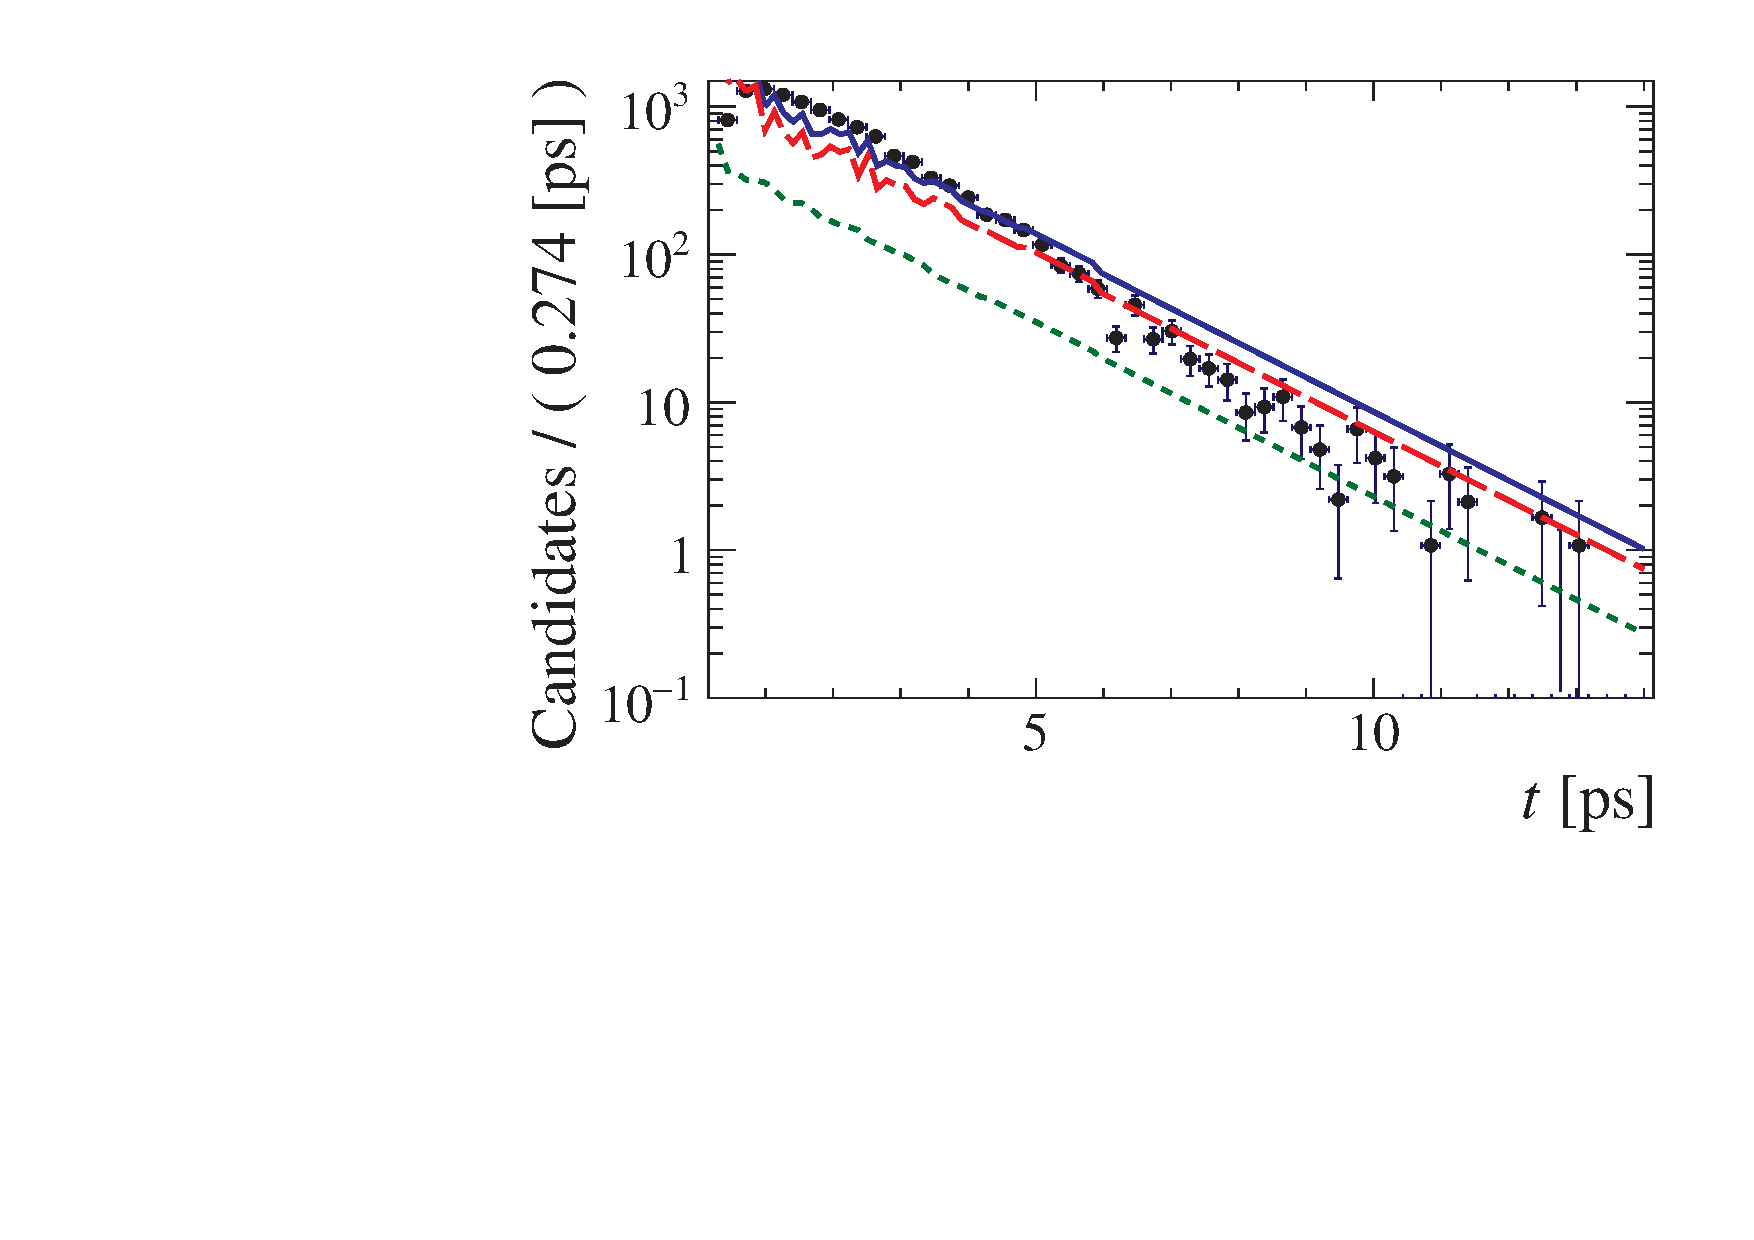
\includegraphics[width=1.\linewidth]{Fit_phis/Overlay_time_All_SubSets.pdf} \\
  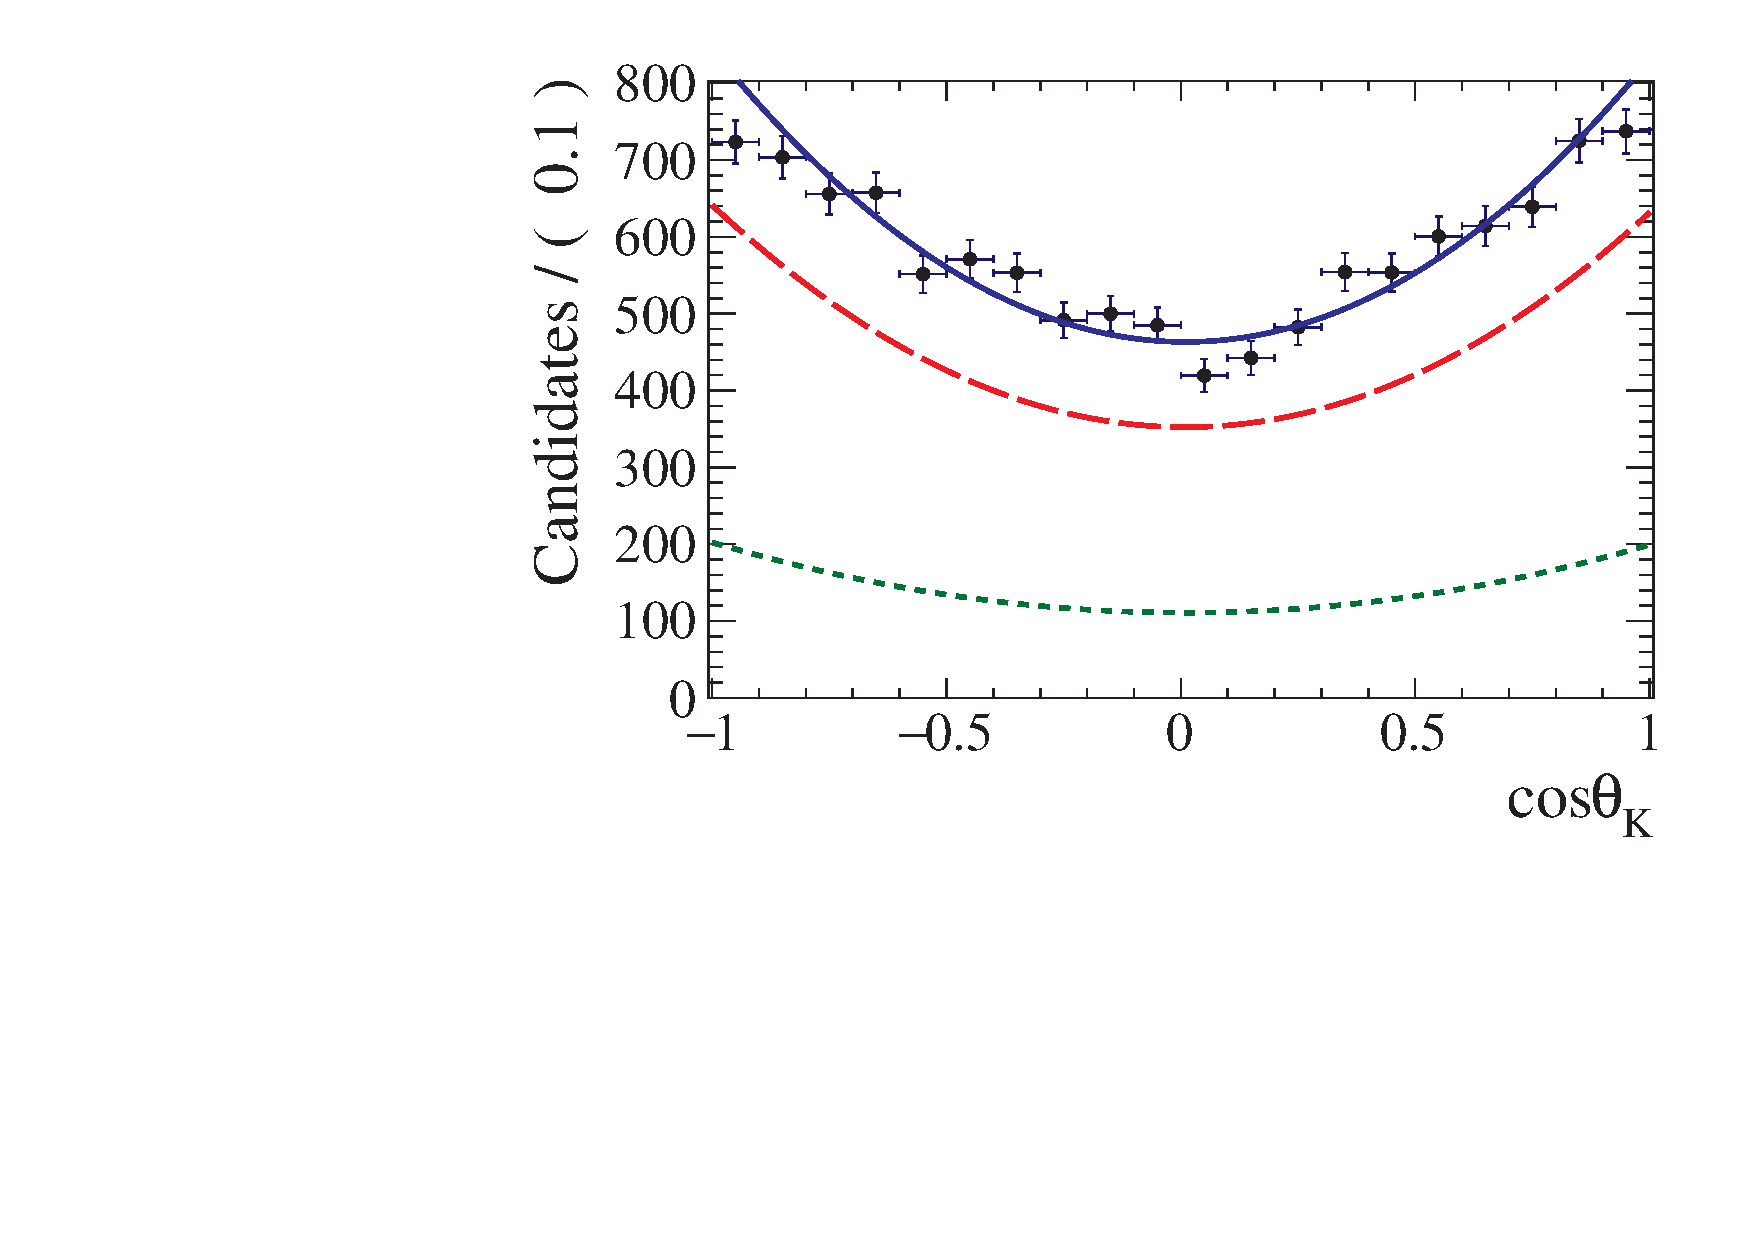
\includegraphics[width=1.\linewidth]{Fit_phis/Overlay_helcosthetaK_All_SubSets.pdf} \\
 \end{minipage}
 \hfill
    \vspace{-5mm}
  \begin{minipage}[ht!]{0.48\linewidth}
 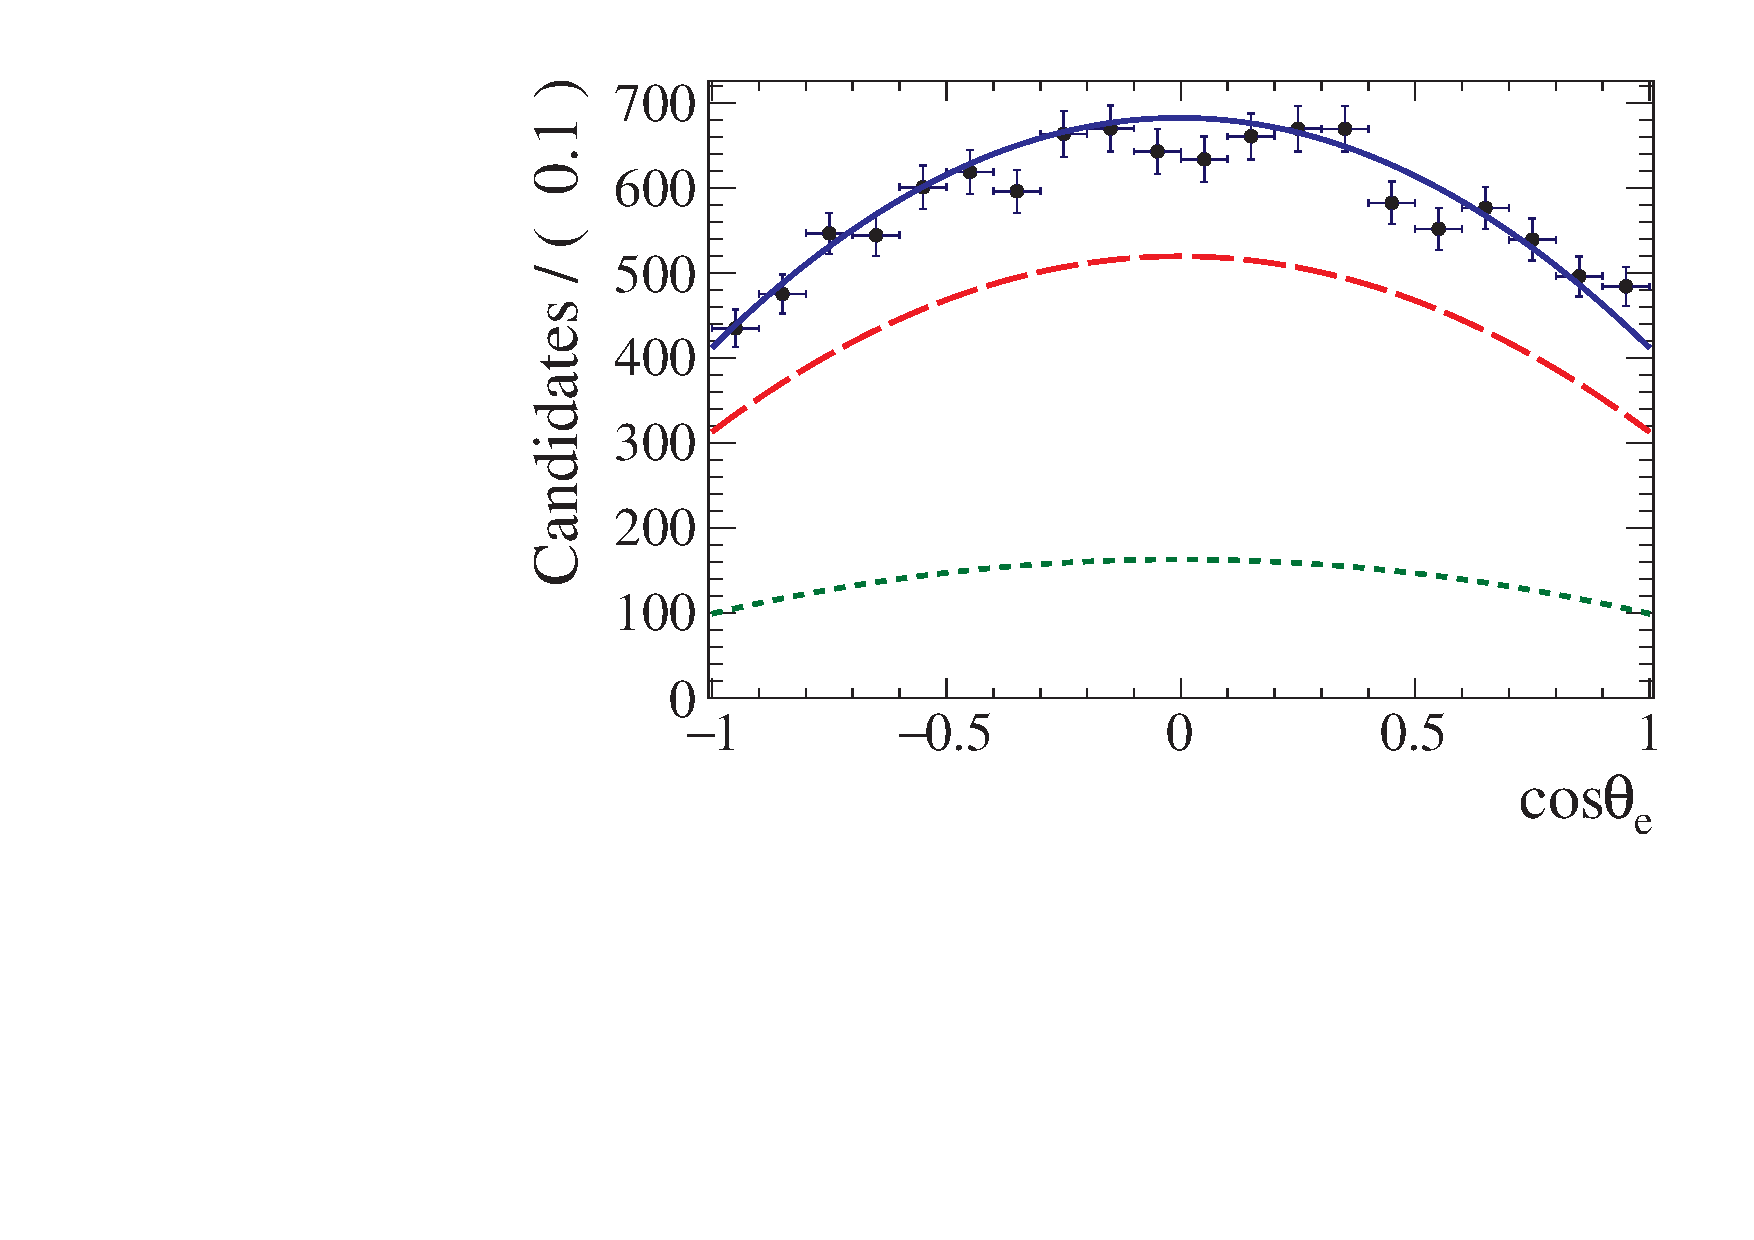
\includegraphics[width=1.\linewidth]{Fit_phis/Overlay_helcosthetaL_All_SubSets.pdf} \\ 
 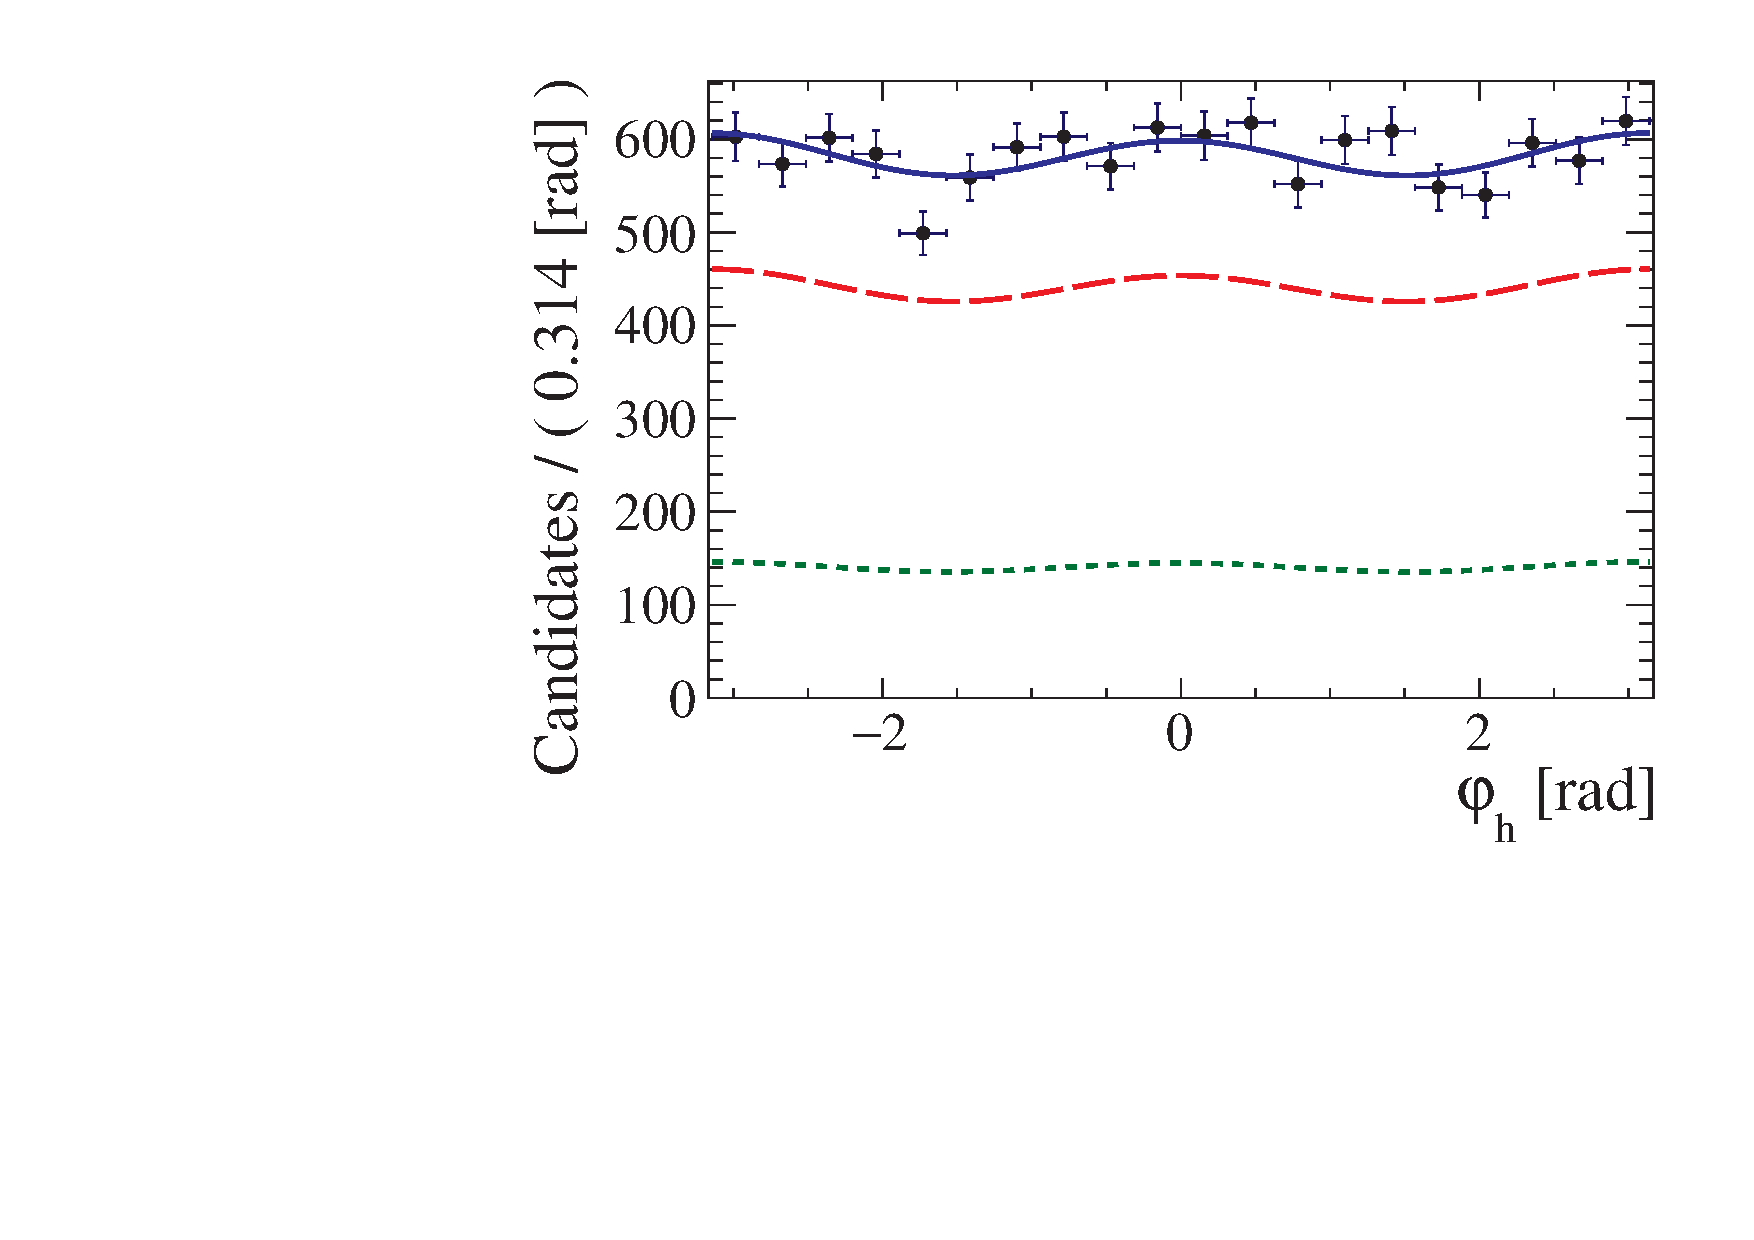
\includegraphics[width=1.\linewidth]{Fit_phis/Overlay_helphi_All_SubSets.pdf} \\
     \end{minipage}
     \vspace*{-0.5cm}
  \end{center}
    \caption{
   The decay time and helicity-angle distributions for $\Bs\to\jpsi(\epem)\phi$ reconstructed candidates (data points) with the one-dimensional projections of the PDF at the maximum likelihood fit. The solid blue line shows the total signal contribution, which is composed of $CP$-even (long dashed red), $CP$-odd (short-dashed green) and S-wave (dash-dotted purple) (not seen) contributions. {\tt Preliminary.}}  
  \label{fig:TimeAngleFit} 
\end{figure}

\clearpage

\section{Systematic uncertainties}\label{sec:SystUnc}

All systematics are described below and a summary is reported in Table~\ref{tab:StatError}. The tagging parameters are allowed to float in the fit (Gaussian constrained within their uncertainty) and thus the systematic uncertainties due to those is propagated into the statistical uncertainties reported on physics parameters.

\subsection{$M(\jpsi(\epem)\phi)$ mass model}

{\it To calculate a new set of event weights obtained from new $M(\jpsi(\epem)\phi)$ fit model.}

\subsection{Angular acceptance}

{\it To add the description of iterative weighting method.}

\subsection{Angular resolution}\label{subsec:Syst:AngRes}

{\it To add the toy studies of the angular resolution.}

\subsection{Decay time resolution}


\subsection{Trigger efficiency}


\subsection{Flavour tagging}\label{subsec:Syst:FT}

{\it The difference between tagging parameters obtained from OS calibration on $\Bp\to\jpsi(\mumu)\Kp$ and $\Bp\to\jpsi(\epem)\Kp$ is assigned as the systematic uncertainty. }


\subsection{Length and momentum scale}

The uncertainty on the LHCb length scale is estimated to be at most 0.020$\%$~\cite{LHCb:ANA-2012-053}, which translates directly in an uncertainty on $\Gs$, $\DGs$ and $\dms$ of 0.020$\%$ with other parameters being unaffected. The momentum scale uncertainty is at most 0.022$\%$~\cite{LHCb:ANA-2012-053}. As it affects both the reconstructed momentum and mass of the $\Bs$ meson, it cancels to a large extent and the resulting effect on $\Gs$ and $\DGs$ is negligible.

\subsection{Contribution from $\Lb$ decays}


\subsection{Fit bias}

{\it A possible bias of the fitting procedure is investigated by generating and fitting many simulated pseudo-experiments of equivalent size to the data sample, generated with physics parameters close to those obtained in the nominal fit.}

\subsection{Further checks}

{\it Additional checks will perform by repeating the nominal fit to data in bins of year of data taking, magnet polarity.}

 
\begin{table}[htb]
  \caption{
   Statistical and systematic uncertainties. The uncertainty for $\phis$ from the fit bias will need to be re-evaluated post-unblinding.
}
    \small{
\begin{center}
\begin{adjustwidth}{-1.5cm}{}
\begin{tabular}{ccccccccc}
Source &$\Gs$ [$\ps^{-1}$]&$\DGs$ [$\ps^{-1}$]&$A_{\hspace{-1pt}\perp}^{2}$&$A_0^2$&$\delta_\parallel$ [$\rad$]&$\delta_\perp$ [$\rad$]&$\phi_s$ [$\rad$]&$\lambda$\\ 		\hline
 Stat. uncert.       &  0.0057    & 0.0155&0.0121&0.0088&0.1759&0.3686&0.1548&0.0261                \\
 \hline
 Mass model      &         &&&&&&&               \\
 Ang. acc.&      &&&&&&&                \\
 Ang. resol.&      &&&&&&&                \\
 Time resol.&      &&&&&&&                \\
 Trigger eff. &      &&&&&&&                \\
 Flav. tag. &  &&&&&&&                \\
 Length, mom. scales&      &&&&&&&                \\
 $\Lb$ background&      &&&&&&&                \\
 Fit bias&      &&&&&&&                \\
 \hline
 Quad. sum of syst.&      &&&&&&&                \\
 Total uncertainties&      &&&&&&&                \\
 \hline
\end{tabular}
\end{adjustwidth}
\end{center}
  }
\label{tab:StatError}
\end{table}

\clearpage

\section{Conclusion}\label{sec:Concl}

We have presented the tagged, time dependent angular analysis of 11 645$\pm$114 $\Bs\to\jpsi(\epem)\phi$ signal candidates with $\jpsi\to\epem$ and in the $M(\Kp\Km)$ region around the $\phi(1020)$ meson. These were recorded in 3~$\invfb$ of $pp$ collision data collected by the $\lhcb$ detector during 2011 and 2012 years. The effective decay time resolution and effective tagging power are 50.2~$\fs$ and 5.2$\%$, respectively. The analysis provides access to a number of different physics parameters including the CP-violating phase, average decay width and decay width difference of the $\Bs$ system as well as the transversely amplitudes and strong phases of the decay. The final results are reported in Table~\ref{tab:FitResultsConcl}. This is the first measurement of the $CP$ content of the $\Bs\to\jpsi(\epem)\phi(\Kp\Km)$ decay and first time that $\phis$ and $\DGs$ have been measured in final state containing the $\jpsi\to\epem$ decay. These measurements will contribute to increased precision in the global average of the $\Bs$ mixing parameters.

\begin{table}[htb]
  \caption{
   The results of the unbinned maximum likelihood fit to the selected $\Bs\to\jpsi(\epem)\phi$ candidates including all acceptance and resolution effects. The tagging calibration parameters and $\dms$ are Gaussian constrained in the fit. The values for $\DGs$ and $\phis$ are blinded. The uncertainty is statistical.
}
    \small{
\begin{center}\begin{tabular}{cc}
Parameter & Fit result and error \\ 		\hline
            $\Gamma_{s}$ [$\ps^{-1}$] &       $X.XXX \pm$ 0.0057                \\
      $\Delta\Gamma_{s}$ [$\ps^{-1}$]&         $X.XXX \pm$  0.0155                \\
$A_{\hspace{-1pt}\perp}^{2}$ &      0.2750 $\pm$   0.0121                \\
             $A_0^2$ &      0.5025 $\pm$  0.0088                \\
  $\delta_\parallel$ [$\rad$] &       3.0092 $\pm$    0.1759                \\
      $\delta_\perp$ [$\rad$] &          3.1086 $\pm$    0.3686                \\
               $F_S$ &     0.0735 $\pm$   0.0167                \\
          $\delta_S$ [$\rad$] &     -0.1093 $\pm$   0.0801                \\
            $\phi_s$ [$\rad$] &      $X.XXX \pm$    0.1548                \\
           $\lambda$ &      0.9836 $\pm$   0.0261                \\
           $\Delta m_s$~[ps$^{-1}$] &       18.176 $\pm$    0.147                \\
\hline
\end{tabular}\end{center}
  }
\label{tab:FitResultsConcl}
\end{table}
\clearpage

\section{To-do list}
\begin{enumerate}
 \item Add comparison plots of kinematic variables for $\Bs\to\jpsi(\mumu)\phi$ and $\Bs\to\jpsi(\epem)\phi$
 \item Complete systematic studies
 \item Perform final fit projections of the decay time and helicity angle 
\end{enumerate}
\clearpage